\documentclass[11pt,oneside,openany]{book}
\pdfinfoomitdate=1
\pdfsuppressptexinfo=15
\pdftrailerid{}
\usepackage[letterpaper,margin=0.78in]{geometry}
\usepackage[T1]{fontenc}
\usepackage[utf8]{inputenc}
\usepackage{lmodern,microtype}
\usepackage{amsmath,amssymb,amsthm,mathtools}
\usepackage{graphicx,booktabs,longtable,tabularx,array,multicol}
\usepackage{xcolor,float,placeins,enumitem,listings,fancyhdr,hyperref}
\usepackage{ragged2e}
\usepackage{titlesec}
\definecolor{Ink}{HTML}{17202A}
\definecolor{Blue}{HTML}{2E86AB}
\definecolor{Teal}{HTML}{2A9D8F}
\definecolor{PaleBlue}{HTML}{E8F1F5}
\definecolor{PaleTeal}{HTML}{E8F4F1}
\definecolor{PaleGold}{HTML}{FCF3D8}
\definecolor{PaleGray}{HTML}{F3F4F6}
\color{Ink}
\hypersetup{
  colorlinks=true,
  linkcolor=Blue,
  urlcolor=Blue,
  citecolor=Blue,
  hypertexnames=false,
  pdftitle={Komorebi PRISM-1: Final Mixed-Representation Architecture Specification},
  pdfauthor={Komorebi P.},
  pdfsubject={Packet-programmable mixed-representation processor for projector-resolved computation, CUDA-compatible Packet IR, PMR-GEMM, exact reconstruction, and local refinement},
  pdfcreator={},pdfproducer={}
}
\pagestyle{fancy}
\fancyhf{}
\fancyfoot[L]{\scriptsize Komorebi PRISM-1}
\fancyfoot[R]{\scriptsize \thepage}
\renewcommand{\headrulewidth}{0pt}
\setlength{\parindent}{0pt}
\setlength{\parskip}{5pt}
\setlength{\emergencystretch}{2em}
\raggedbottom
\titleclass{\chapter}{straight}
\titleformat{\chapter}[hang]
  {\normalfont\huge\bfseries\color{Ink}}
  {\thechapter}
  {0.75em}
  {}
\titlespacing*{\chapter}{0pt}{2.2ex plus 0.5ex minus 0.2ex}{1.2ex}
\graphicspath{{figures/}}
\setlist[itemize]{leftmargin=1.35em,itemsep=2pt,topsep=3pt}
\setlist[enumerate]{leftmargin=1.55em,itemsep=3pt,topsep=3pt}
\newcolumntype{Y}{>{\RaggedRight\arraybackslash}X}
\newcolumntype{L}[1]{>{\RaggedRight\arraybackslash}p{#1}}
\newtheorem{definition}{Definition}[chapter]
\newtheorem{theorem}[definition]{Theorem}
\newtheorem{proposition}[definition]{Proposition}
\newtheorem{corollary}[definition]{Corollary}
\newtheorem{certificate}[definition]{Certificate}
\theoremstyle{remark}
\newtheorem{remark}[definition]{Remark}
\newtheorem{boundary}[definition]{Boundary}
\newcommand{\Pcal}{\mathcal P}
\newcommand{\Acal}{\mathcal A}
\newcommand{\Scal}{\mathcal S}
\newcommand{\Rcal}{\mathcal R}
\newcommand{\Tcal}{\mathcal T}
\newcommand{\norm}[1]{\left\lVert #1\right\rVert}
\newcommand{\Callout}[1]{\noindent\colorbox{PaleBlue}{\parbox{0.965\linewidth}{\vspace{3pt}\small\RaggedRight #1\par\vspace{3pt}}}}
\lstset{
  basicstyle=\ttfamily\scriptsize,
  breaklines=true,
  showstringspaces=false,
  frame=single,
  columns=fullflexible,
  tabsize=2
}
\begin{document}

\begin{titlepage}
\centering
\vspace*{0.55in}
{\Large\color{Blue}\bfseries PROJECTOR-RESOLVED SEED CALCULUS\par}
\vspace{0.20in}
{\Huge\bfseries Komorebi PRISM-1\par}
\vspace{0.10in}
{\LARGE\bfseries A Packet-Programmable Mixed-Representation Processor\par}
\vspace{0.18in}
{\Large CUDA-like packet execution, PMR--GEMM, transform atlases, structured operators, edge recovery, and certified reconstruction\par}
\vspace{0.45in}
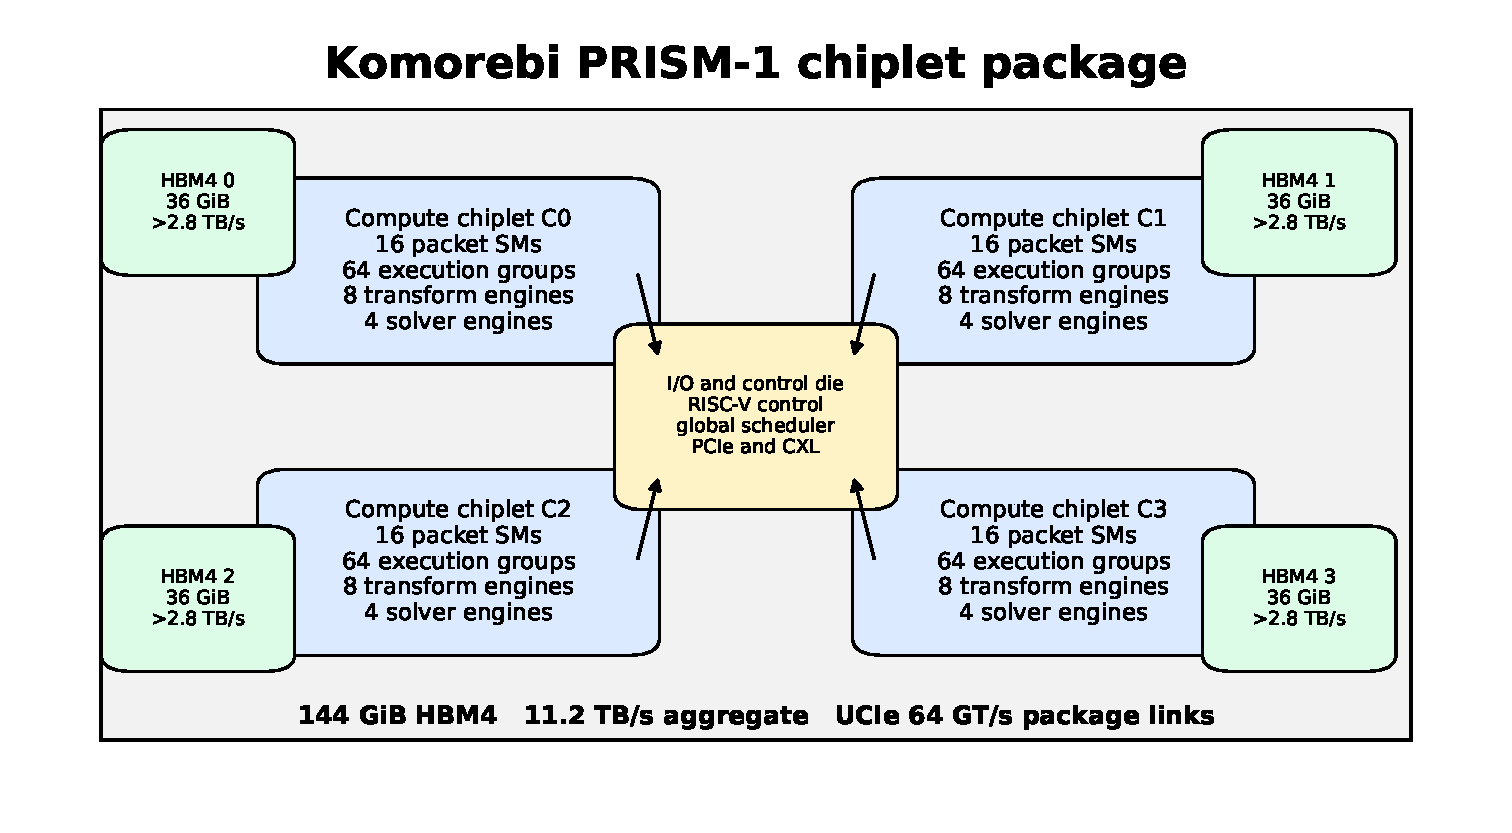
\includegraphics[width=0.92\linewidth,height=3.7in,keepaspectratio]{01_package_architecture.pdf}
\vfill
{\Large Komorebi P.\par}
\vspace{0.24in}
{\large Final updated architecture, programming model, CUDA compatibility path, compiler contract, verification plan, and executable model\par}
\end{titlepage}

\frontmatter
\clearpage
\chapter*{Abstract}
\addcontentsline{toc}{chapter}{Abstract}
Komorebi PRISM-1 is a programmable chiplet accelerator for computations whose useful form is known before execution. Its native objects are packet graphs, transform plans, block operators, low-rank factors, Kronecker products, sparse factor chains, refinement trees, small algebraic systems, and reconstruction certificates. A dense array is one possible representation. The architecture never requires one to exist.

The final reference design contains four compute chiplets, 64 Packet Streaming Multiprocessors, 256 packet execution groups, configurable transform engines, resident small solvers, exact arithmetic support, 192 MiB of on-package SRAM, and four HBM4 stacks. Each Packet Streaming Multiprocessor schedules packet warps across four execution groups and a shared scratchpad. The execution model is CUDA-like in its hierarchy and programmability, but it keeps atlas identity, parent-child relations, output contracts, precision weights, and certificate state visible to hardware.

The compiler begins with Packet IR and chooses among explicit dense, block, block-sparse, low-rank, block-diagonal-plus-low-rank, Kronecker, sparse-chain, transform-domain, and packet-graph plans. PMR--GEMM supplies the recursive mixed-representation planner. The same Packet IR can lower to a CUDA compatibility backend or to PRISM. Earlier CUDA implementations already establish the software path through grouped matrix kernels, CUDA Graph replay, asynchronous transfers, FFT and sparse libraries, compressed products, Woodbury solves, and packetwise mixed precision.

The paper specifies the package, Packet Streaming Multiprocessor, memory hierarchy, network, command format, compiler, output contracts, certificate protocol, performance accounting, FPGA path, and verification plan. Existing CUDA measurements are kept separate from PRISM architecture estimates. Representation gain, kernel gain, architecture gain, and amortization are reported as different quantities. The design remains an architecture specification. It is not fabricated silicon and it does not claim measured PRISM frequency, power, or throughput.

\clearpage
\chapter*{Status and scope}
\addcontentsline{toc}{chapter}{Status and scope}
This is the final updated architecture draft. The packet types, Packet IR, output contracts, command groups, Packet Streaming Multiprocessor boundary, memory hierarchy, compiler routes, error-budget rules, CUDA compatibility path, and verification ladder are specified. Circuit timing, SRAM banking, NoC virtual channels, floorplanning, hardened interface IP, and process-node choices remain implementation work.

The package baseline uses public interfaces that are available or specified at the time of this draft. UCIe 3.0 includes 48 and 64 GT/s die-to-die classes. PCIe 7.0 specifies 128 GT/s. Micron lists 36 GB HBM4 in high-volume production with bandwidth above 2.8 TB/s per stack. The management cores use the ratified RISC-V vector programming model. These facts establish a plausible component baseline. They do not validate the PRISM microarchitecture.

\Callout{PRISM-1 does not preserve a dense matrix. It preserves the mathematical output contract. A packet program may remain a factor graph, transform plan, sparse chain, low-rank correction, or executable operator from beginning to end.}

\clearpage
\chapter*{Executive summary}
\addcontentsline{toc}{chapter}{Executive summary}
The design is built around seven practical decisions.
\begin{enumerate}
\item Keep representation visible from the calculus front end to the command queue.
\item Treat a dense array as an optional leaf or requested output, not as mandatory machine state.
\item Use one Packet IR for the CUDA backend and the PRISM backend.
\item Schedule packet warps on programmable Packet Streaming Multiprocessors.
\item Keep factors, transform plans, and packet graphs resident whenever later stages can consume them directly.
\item Keep exact archives separate from compact predictive states.
\item Make residuals and error bounds part of the commit path.
\end{enumerate}

The software basis already exists. On the recorded RTX 3070 Ti Laptop GPU, an equal-block packet operator was measured at $0.046032$ ms and ran $14.8919\times$ faster than its matched device-resident dense GPU row. A BDLR packet path with CUDA Graph replay was measured at $0.079872$ ms and ran $10.9355\times$ faster than the matched dense GPU row. Graph replay improved the same packet representation by about $1.218\times$. A compressed BDLR product took $0.1582$ ms, while materializing the output took $0.5073$ ms. These measurements show that the calculus can already execute on CUDA without preserving a dense matrix.

PRISM addresses the work left after the representation has already improved. Its likely advantages come from resident factor reuse, packet gather and scatter, transform-to-solver handoff, grouped small-block dispatch, local refinement, deterministic graph replay, and certificate accumulation. The architecture model estimates gains of $2.96\times$ for the resident edge-recovery chain, $1.64\times$ for a fused multi-atlas path, and $1.42\times$ for a shape-batched Bayesian portfolio. Those are architecture estimates. They are not silicon measurements.

The earlier $37.8\times$ dense-route comparison is retained only as a total route model. It combines a better representation with a different architecture. It is not reported as a PRISM-over-CUDA architecture gain.

\clearpage
\tableofcontents
\clearpage
\listoffigures

\clearpage
\mainmatter
\chapter{Design brief}

\section{The design problem}
Many computations begin with structure that disappears before hardware sees the job. A block operator becomes one dense matrix. A Fourier or wavelet atlas becomes an unnamed array. A parent packet and its children become unrelated buffers. A low-rank correction is materialized even when every later stage could have consumed its factors.

PRISM-1 keeps those relations explicit. The architecture is useful only when that choice saves arithmetic, storage, data movement, or scheduling work. The compiler is allowed to decline the packet path.

\section{Required behavior}
\begin{longtable}{L{0.25\linewidth}L{0.66\linewidth}}
\toprule
Requirement & Meaning \\
\midrule
\endfirsthead
\toprule
Requirement & Meaning \\
\midrule
\endhead
Exact packet synthesis & A declared complete packet family must reconstruct the original object within the stated numerical format \\
Typed transfer & Every operator edge retains its source packet, destination packet, shape, rank, precision, and sensitivity \\
Local refinement & Replacing one parent by a child graph must not force unrelated tasks to be regenerated \\
Representation preservation & Block, sparse, low-rank, Kronecker, factor-chain, transform, and packet-graph forms remain executable without an explicit full array \\
Provisional execution & Results that require a certificate remain hidden from downstream work until the check passes \\
Deterministic replay & Selected graph regions can use fixed reductions and stable descriptors for reproducible reruns \\
Graceful rejection & Work with weak structure is routed to the CUDA backend, a general-purpose path, or a generic leaf \\
\bottomrule
\end{longtable}

\section{Design rules}
\begin{enumerate}
\item The mathematical object and its storage representation are not assumed to be the same thing.
\item A packet descriptor is part of the architectural state, not debugging metadata.
\item An application result, a factor graph, a transform plan, and an explicit array are different output contracts.
\item A numerical result is not committed merely because the kernel finished.
\item A failed certificate should identify the local graph region that needs replay or refinement.
\item The first prototype should preserve the final command and descriptor formats even if it implements fewer engines.
\end{enumerate}

\begin{figure}[H]
\centering
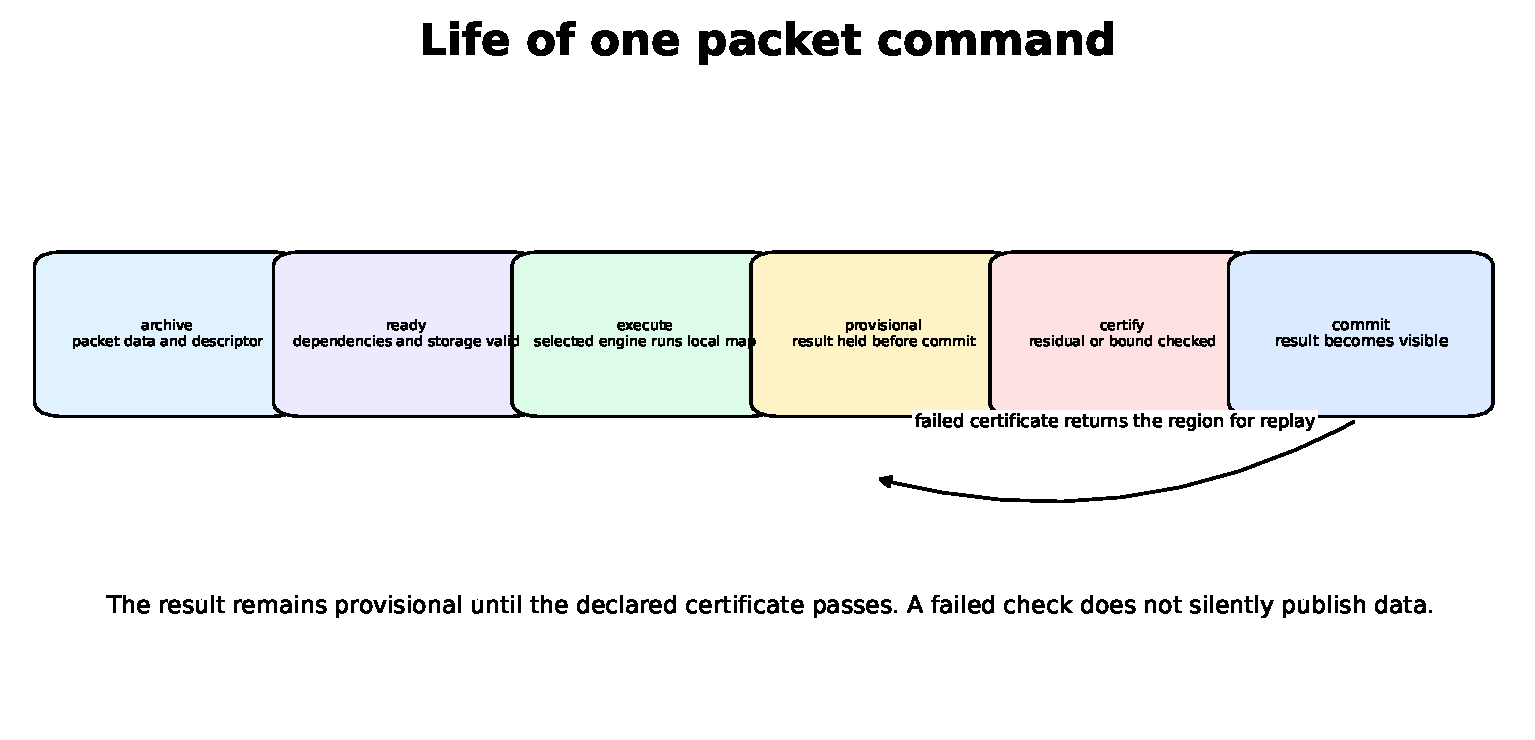
\includegraphics[width=0.98\linewidth]{24_packet_lifecycle.pdf}
\caption{One packet command from archive to commit. The provisional state prevents an unchecked result from becoming visible to downstream work.}
\end{figure}

\begin{figure}[H]
\centering
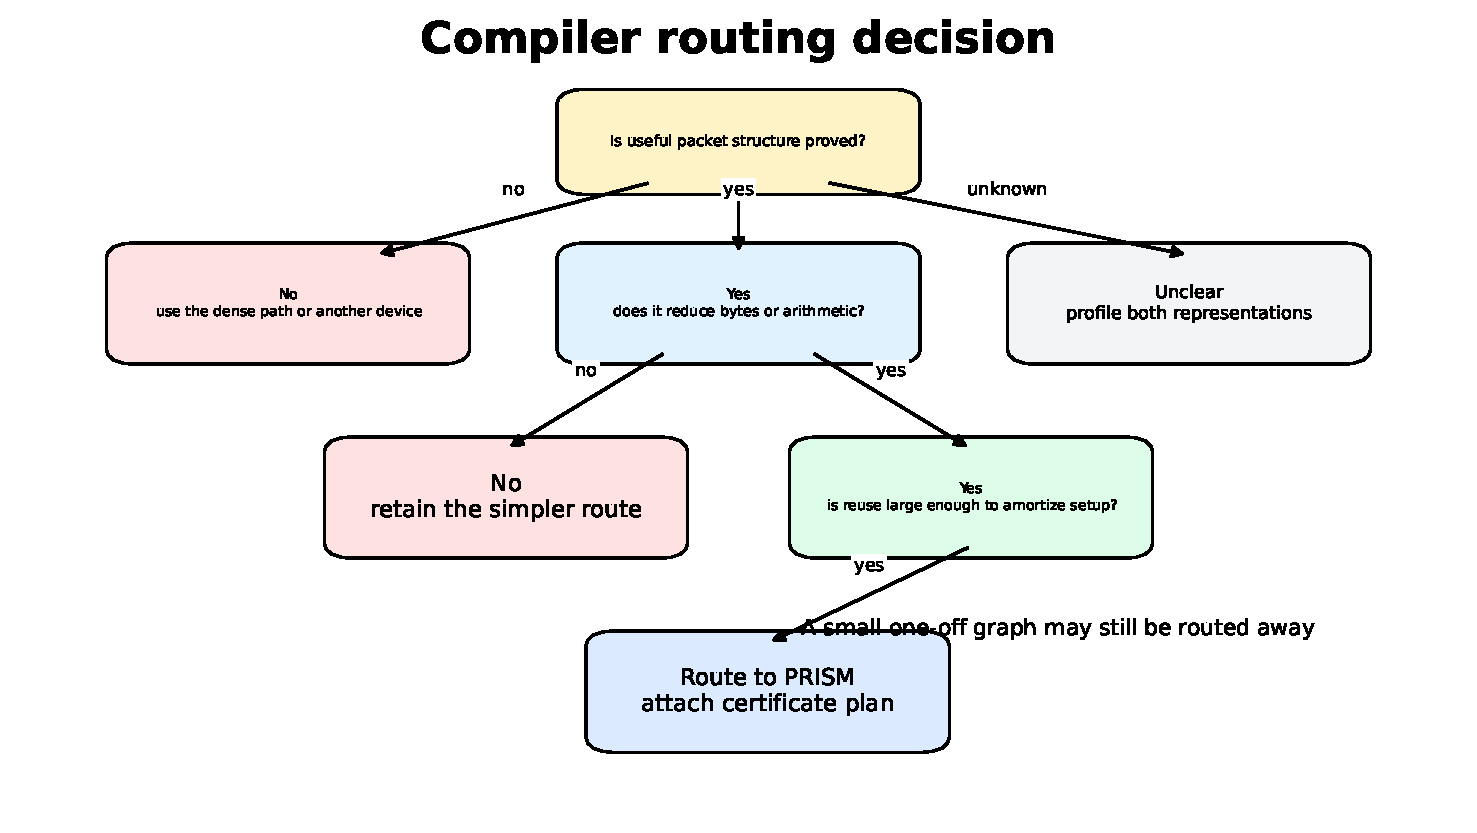
\includegraphics[width=0.94\linewidth]{25_workload_router.pdf}
\caption{The compiler is expected to route weakly structured work away from the packet path.}
\end{figure}

\section{What this design does not promise}
PRISM-1 is not a universal replacement for a GPU or CPU. It does not claim a better asymptotic exponent for generic dense linear algebra. It does not claim that every operator has a useful structured representation. It does not treat modeled roofline numbers as measured performance. Its case rests on workloads where structure is real, reusable, and large enough to amortize descriptor, planning, and scheduling cost.

\chapter{Why this chip exists}

\section{The representation is part of the computation}
A conventional accelerator usually receives a tensor after the representation has already been chosen. It may execute that tensor well and still miss the simpler object underneath it. The operator may be block diagonal, block sparse, low rank, generated by a transform, or recoverable from a much smaller packet graph.

Projector-resolved computation starts before that flattening step. Let
\[
X=\bigoplus_{\alpha\in I}X_\alpha,
\qquad
P_\alpha P_\beta=\delta_{\alpha\beta}P_\alpha,
\qquad
\sum_{\alpha\in I}P_\alpha=I.
\]
For an operator $T:X\to X$, the native objects are the transfer blocks
\[
T_{\beta\alpha}=P_\beta T P_\alpha.
\]
The complete operator is reconstructed by
\[
\boxed{T=\sum_{\alpha,\beta}T_{\beta\alpha}.}
\]
The zero pattern, block shapes, rank structure, parent-child relations, and packet sensitivities are part of the problem. PRISM-1 carries them into the execution model instead of asking software to rediscover them after every kernel boundary.

\section{The target workload}
The design focuses on operations that recur throughout the calculus:
\begin{itemize}
\item residue and phase projectors
\item polyphase extraction and interleaving
\item Fourier, cosine, Hadamard, and wavelet atlases
\item packet-tree refinement and coarsening
\item block-diagonal and block-sparse transfers
\item block diagonal plus low rank operators
\item exact compressed products and Woodbury solves
\item small Hankel, QR, SVD, root, and Vandermonde problems
\item nonlinear packet interactions and memory kernels
\item conjugate Bayesian regression and posterior mixtures
\item exact modular, CRT, and valuation operations
\item residual and error-bound certificates
\end{itemize}

\begin{figure}[H]
\centering
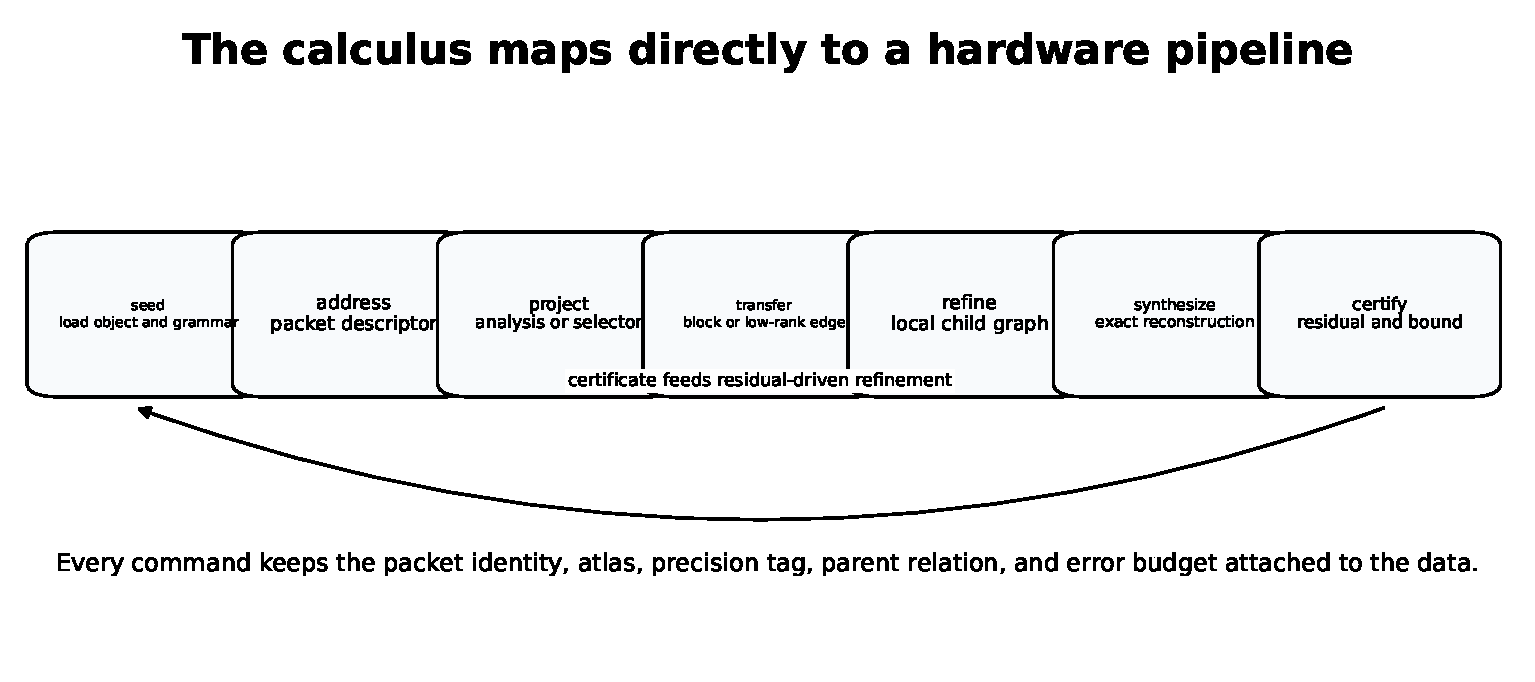
\includegraphics[width=0.98\linewidth]{03_calculus_pipeline.pdf}
\caption{The seed-calculus operations become a hardware pipeline without losing their mathematical type.}
\end{figure}

\section{What the chip is not}
PRISM-1 should not be used simply because a packet description exists. A generic dense matrix with no reusable structure may run better through a conventional library path. A tiny one-off transform may not amortize descriptor setup. A graph that changes completely at every step may not benefit from replay. The compiler should reject or reroute those cases.

\section{No dense preservation requirement}
The architecture does not begin with a dense matrix and try to compress it after the fact. It begins with a typed operator. That operator may be represented as
\[
\boxed{
\begin{aligned}
\mathfrak R=\{&\text{explicit array},\ \text{block},\ \text{block sparse},\ \text{low rank},\ \text{BDLR},\\
&\text{Kronecker},\ \text{sparse chain},\ \text{transform plan},\ \text{packet graph}\}.
\end{aligned}
}
\]
A dense representation is useful when no better form exists or when a downstream user explicitly asks for every entry. It is not a state that the chip must preserve.

\begin{figure}[H]
\centering
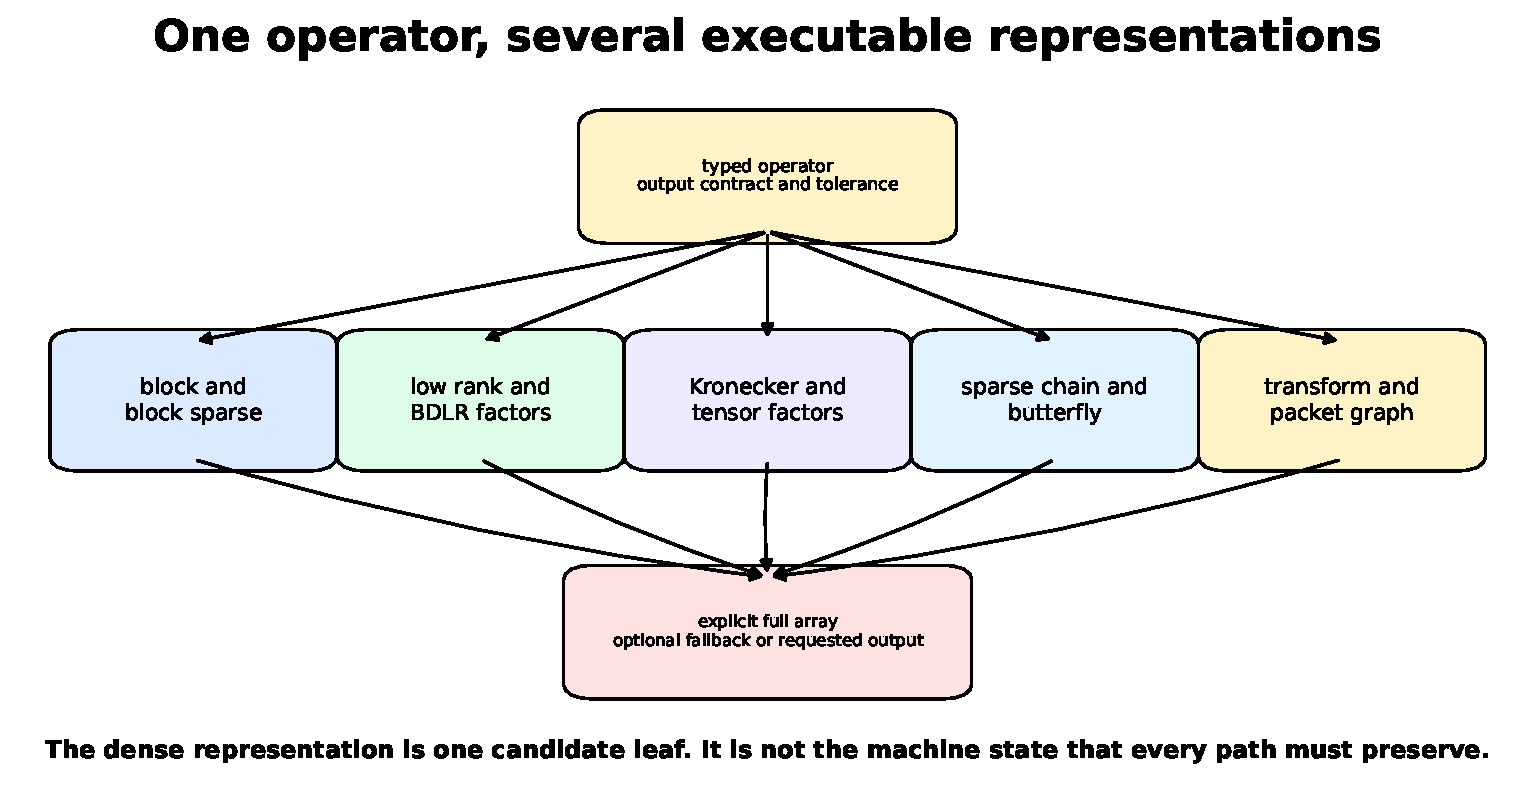
\includegraphics[width=0.97\linewidth]{38_mixed_representation_space.pdf}
\caption{One operator may have several executable representations. The explicit array is one optional leaf.}
\end{figure}

\section{CUDA-like execution hierarchy}
CUDA made heterogeneous arithmetic programmable through a hierarchy of lanes, warps, blocks, grids, and memories. PRISM uses an analogous execution hierarchy while retaining the mathematical structure that CUDA kernels normally receive only through software conventions:
\[
\boxed{
\text{lane}
\longrightarrow
\text{packet warp}
\longrightarrow
\text{execution group}
\longrightarrow
\text{Packet Streaming Multiprocessor}
\longrightarrow
\text{packet graph}.
}
\]
A packet warp may invoke a matrix group, vector lanes, a transform engine, a small solver, exact arithmetic, or a memory operator. The representation router chooses the form declared by Packet IR. Several forms may appear in one graph.

\section{The CUDA implementation is the software foundation}
The packet algorithms already run on CUDA. Equal blocks are stacked and sent to grouped or batched matrix kernels. BDLR application uses a block batch followed by two low-rank contractions. Repeated graphs use CUDA Graph replay. Fourier and sparse stages use established libraries. The runtime keeps factors resident when the output contract allows it.

This matters for the chip design. PRISM is not a replacement for the CUDA algorithms. It is a hardware target for the same Packet IR. The CUDA backend remains the development platform, portability path, and matched comparison.

\begin{figure}[H]
\centering
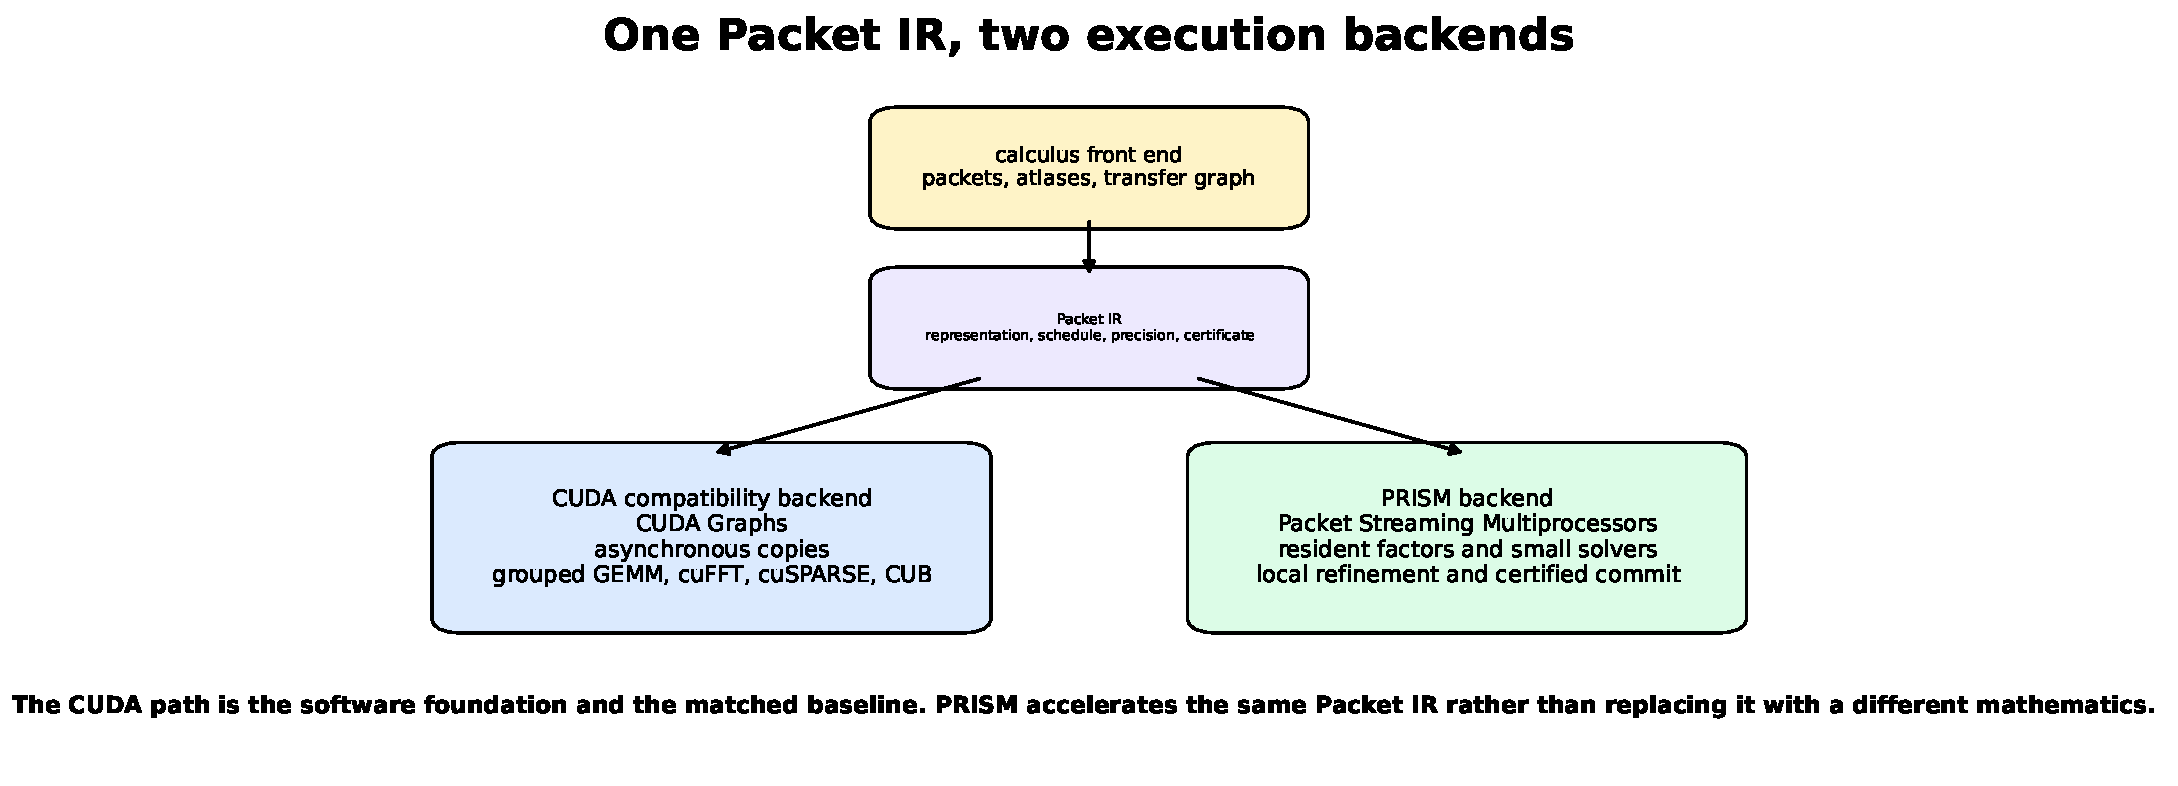
\includegraphics[width=0.94\linewidth]{40_shared_packet_ir.pdf}
\caption{The CUDA and PRISM backends execute the same Packet IR and preserve the same output contracts.}
\end{figure}

\chapter{Mixed-representation execution}

\section{Output contracts}
A computation is not defined only by the numerical entries of a hypothetical matrix. The caller also specifies what must be returned. PRISM uses five principal contracts:
\begin{enumerate}
\item apply an operator to one or more vectors
\item return a compressed operator
\item return a factor or packet graph
\item return a transform plan
\item return every entry of an explicit array
\end{enumerate}
Only the fifth contract forces materialization.

\begin{figure}[H]
\centering
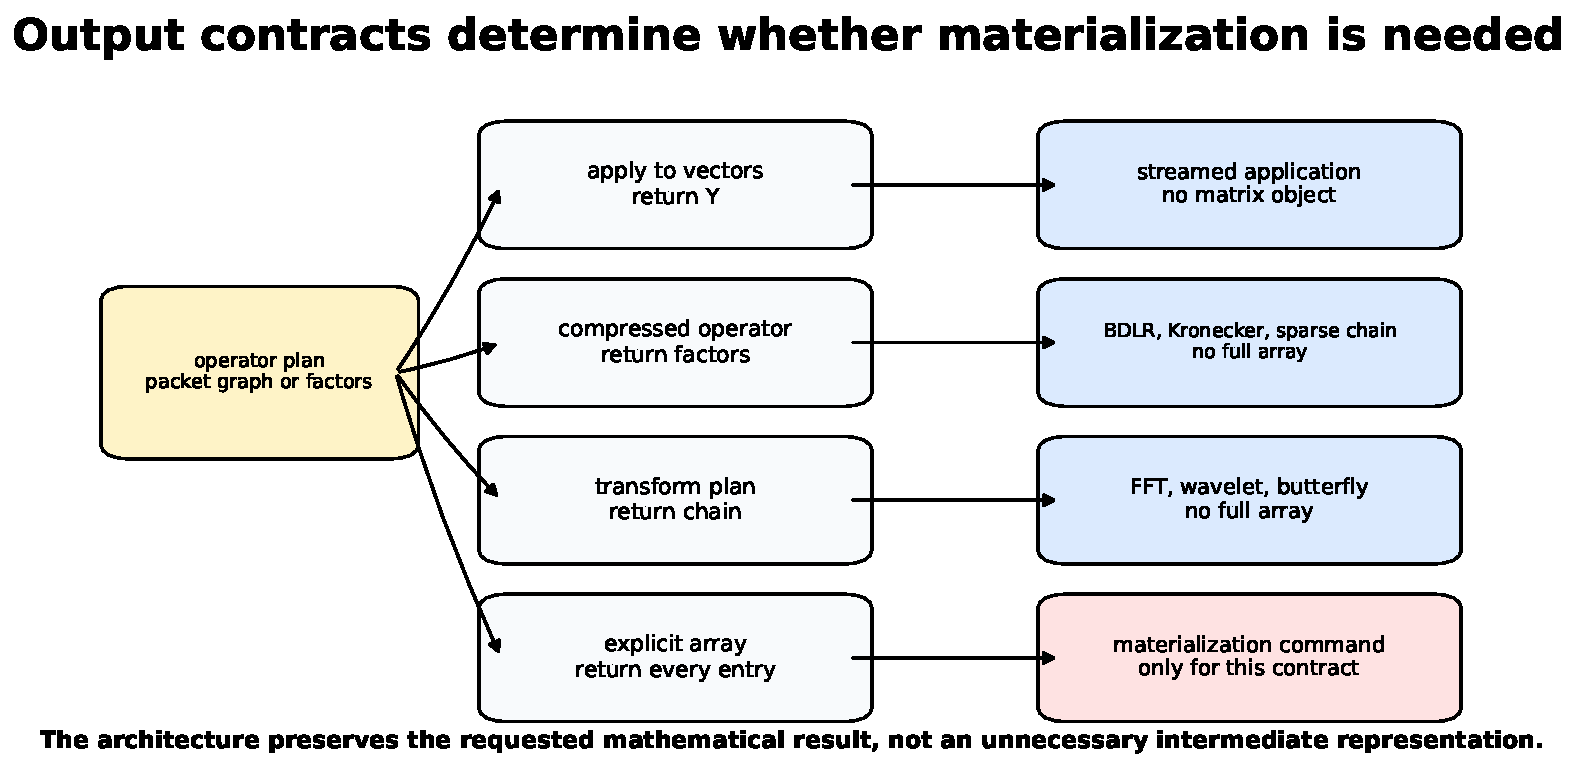
\includegraphics[width=0.96\linewidth]{42_output_contracts.pdf}
\caption{Materialization is required only when the requested output is the explicit full array.}
\end{figure}

\section{Compatible middle bases}
The intermediate basis is part of the optimization. For any invertible $S$,
\[
AB=(AS)(S^{-1}B).
\]
Suppose
\[
A=L D_A S^{-1},
\qquad
B=S D_B R.
\]
Then
\[
\boxed{AB=L(D_AD_B)R.}
\]
When $L$, $S$, and $R$ have fast application and $D_A$, $D_B$ are block diagonal, the product inherits the blockwise cost plus the transform costs. Fourier diagonalization of circulants, simultaneous diagonalization, symmetry sectors, and tensor factorizations are instances of the same rule.

\section{Sparse chains and transform plans}
A matrix may be dense as an array and cheap as an operator. If
\[
A=F_LF_{L-1}\cdots F_1
\]
and each factor has $O(n)$ nonzero entries, then applying $A$ costs $O(nL)$. If $L=O(\log n)$, the cost is $O(n\log n)$. FFT and butterfly operators fit this pattern. PRISM stores the factor chain and executes it. It does not store the dense array represented by the chain.

\section{PMR--GEMM}
Packet Mixed-Representation GEMM is the compiler planner for operator products. It accepts the operator pair, tolerance, output contract, candidate transforms, and packet tree. At each node it may use a generic leaf, a low-rank contraction, a Kronecker identity, a sparse factor chain, a transform-domain rule, or a recursive split.

For a fixed candidate tree, each choice $o$ has a local cost $c(o)$, a local error $e(o)$, and zero or more children. The planner evaluates
\[
J(v)=\min_{o\in\mathcal O_v}
\left[
 c(o)+\lambda e(o)^2+
 \sum_{u\in\operatorname{child}(o)}J(u)
\right].
\]
Bottom-up evaluation is globally optimal on the fixed tree because every feasible plan consists of one local choice followed by feasible child plans.

\begin{figure}[H]
\centering
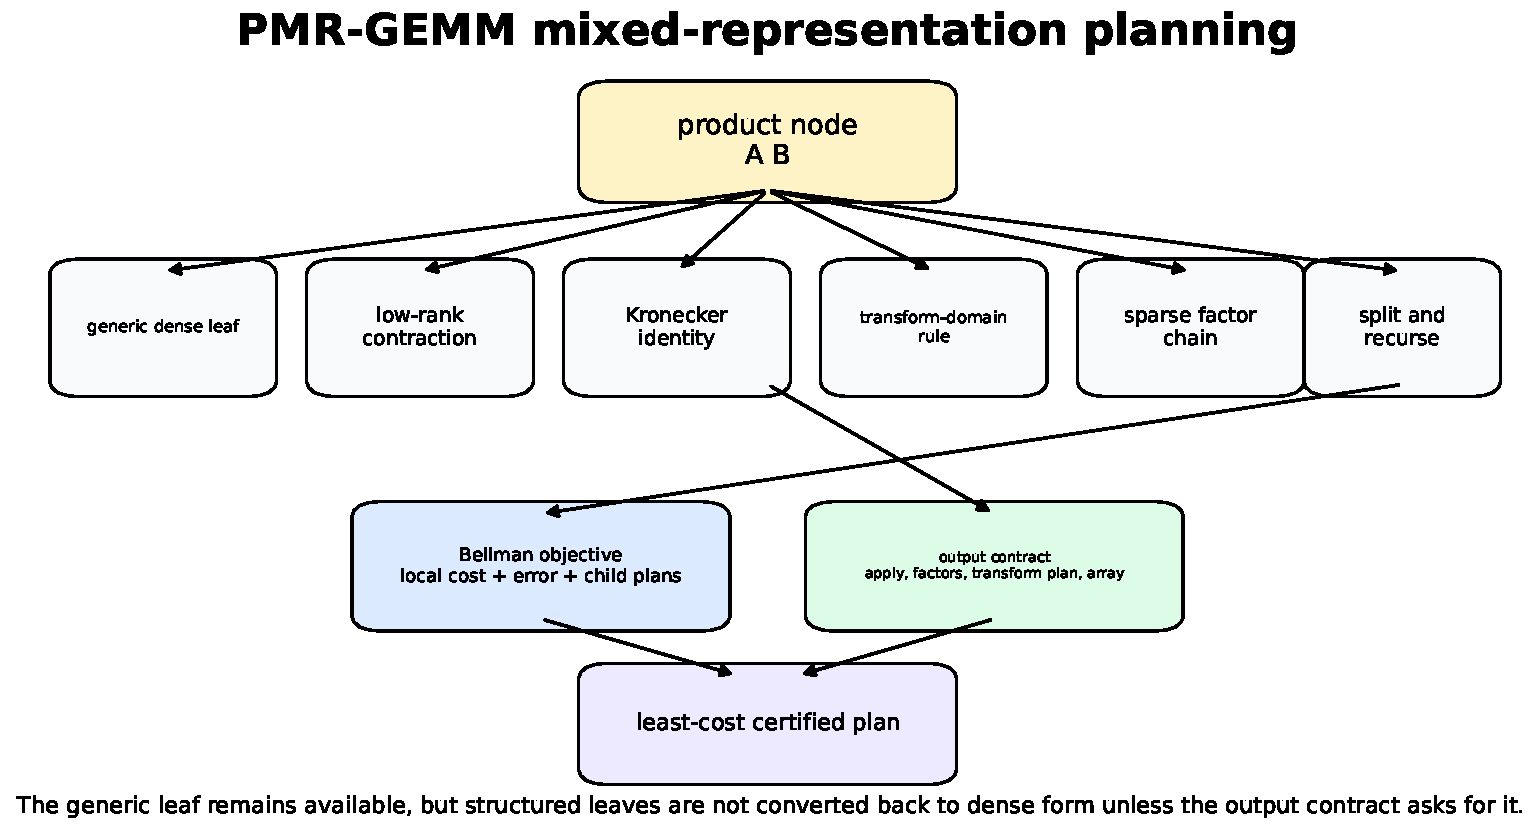
\includegraphics[width=0.97\linewidth]{39_pmr_gemm_planner.pdf}
\caption{PMR--GEMM chooses the least-cost certified plan that satisfies the requested output contract.}
\end{figure}

\section{Hybrid fallback}
The planner always includes a generic leaf. This protects the worst case. Random dense matrices with no useful local rank, transform, tensor, or packet structure return to the generic path. The architecture is strongest when the mixed plan eliminates arithmetic or movement. It does not claim that naming a packet makes an operator cheaper.

\chapter{Reference package}

\section{Chiplet organization}
The reference package contains four compute chiplets, one I/O and control die, and four HBM4 stacks. Each compute chiplet contains 16 Packet Streaming Multiprocessors. Every multiprocessor contains four packet execution groups, giving 64 execution groups per chiplet and 256 across the package. Each chiplet also contains eight transform engines, four small-solver engines, one exact arithmetic cluster, and 16 MiB of shared SRAM.

\begin{figure}[H]
\centering
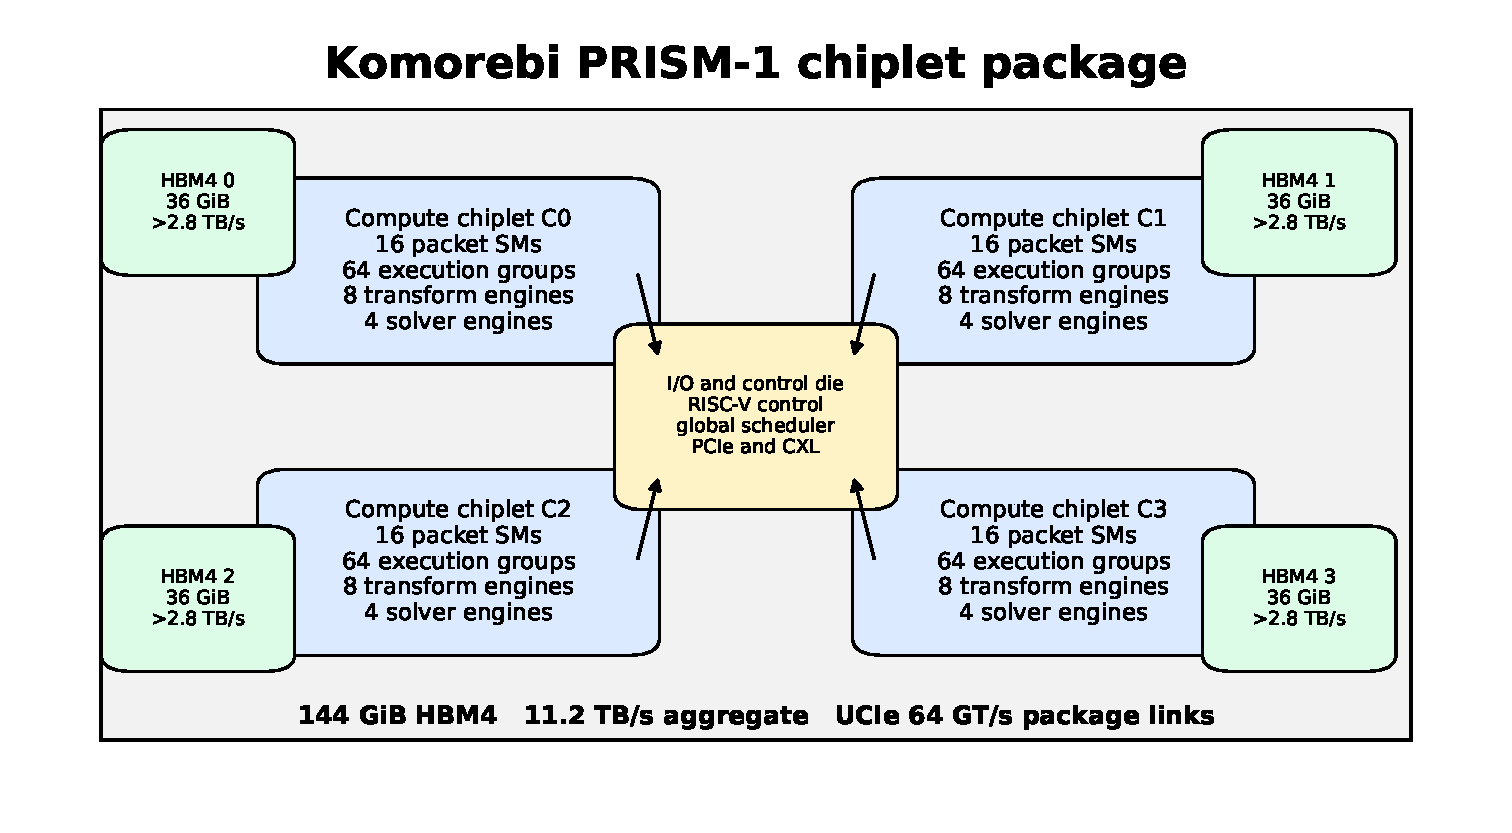
\includegraphics[width=0.98\linewidth]{01_package_architecture.pdf}
\caption{The reference PRISM-1 package. The center die carries host I/O, global scheduling, RISC-V control, security, and telemetry.}
\end{figure}

\section{Reference targets}
\begin{table}[H]
\centering
\caption{Reference architecture targets. These values belong to the model, not measured silicon.}
\begin{tabularx}{0.94\linewidth}{L{0.42\linewidth}Y}
\toprule
Property & Reference target \\
\midrule
Compute chiplets & 4 \\
Packet Streaming Multiprocessors & 64 \\
Packet execution groups & 256 \\
Execution group array & $16\times16$ matrix array plus vector lanes \\
Clock & 1.5 GHz \\
PSM scratchpad & 2 MiB across four independently banked regions \\
Shared SRAM & 16 MiB per compute chiplet \\
Total local and shared SRAM & 192 MiB \\
Transform engines & 32 \\
Small-solver engines & 16 \\
Exact arithmetic clusters & 4 \\
HBM4 & 4 stacks, 144 GiB total \\
Aggregate HBM bandwidth & greater than 11.2 TB/s \\
Package fabric & UCIe 3.0 class, up to 64 GT/s \\
Host interface & PCIe 7.0 x16 class, optional CXL \\
Reference power envelope & 500 W \\
\bottomrule
\end{tabularx}
\end{table}

\section{Compute-chiplet layout}
The reference chiplet places a $4\times4$ mesh of Packet Streaming Multiprocessors at its center. Every multiprocessor contains four execution groups, giving 64 matrix and vector groups per chiplet. Transform engines sit along one edge, solver engines along another, shared SRAM banks line the data path, and the UCIe router occupies a package-facing edge. This is a planning floorplan rather than a placed design. Its purpose is to make communication and locality assumptions visible early.

\begin{figure}[H]
\centering
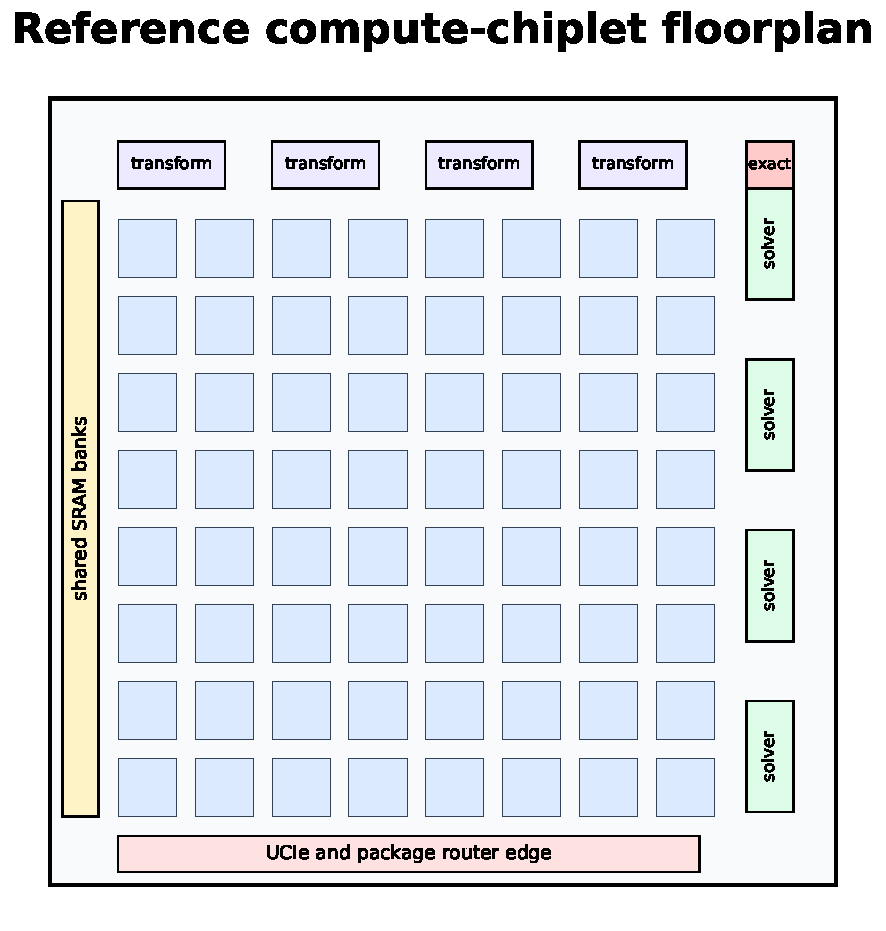
\includegraphics[width=0.82\linewidth]{26_chiplet_floorplan.pdf}
\caption{Reference compute-chiplet floorplan. The drawing is functional. Bank count, channel width, and physical dimensions remain open.}
\end{figure}

\section{Bandwidth balance}
The host link is intended for graph submission, coarse data movement, and result return. It is not the steady-state path for every packet. Reusable graphs, factors, and active atlases should remain in HBM or on-package SRAM. The modeled package fabric is wider than aggregate HBM bandwidth so inter-chiplet traffic does not become an immediate architectural bottleneck in the reference configuration.

\begin{figure}[H]
\centering
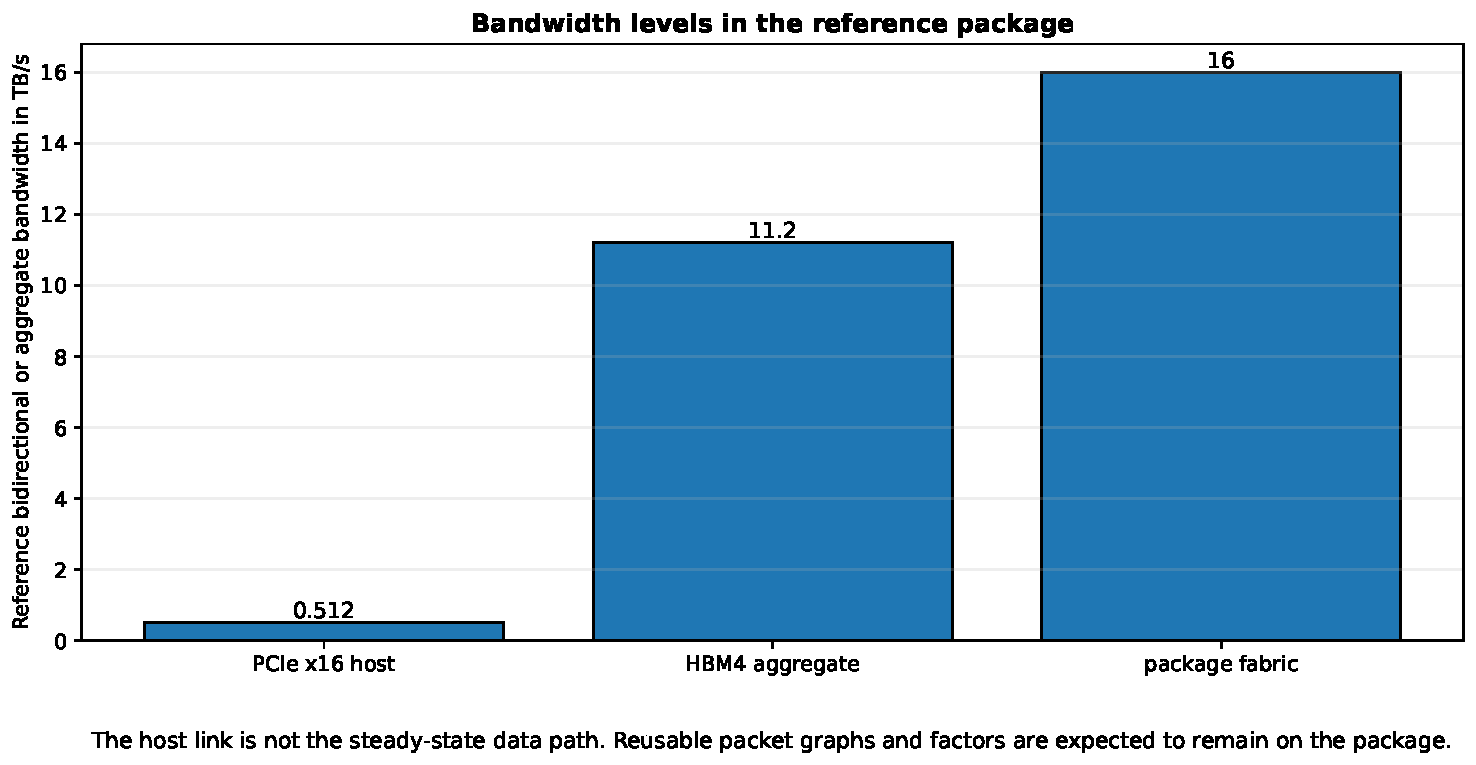
\includegraphics[width=0.78\linewidth]{27_bandwidth_budget.pdf}
\caption{Reference bandwidth levels. Local SRAM bandwidth is a circuit-level target and is not assigned a final number in this draft.}
\end{figure}

\section{Scale-down configurations}
The same Packet IR, commands, and descriptors support smaller devices.
\begin{table}[H]
\centering
\caption{Suggested development configurations.}
\begin{tabularx}{0.96\linewidth}{L{0.23\linewidth}rrrrY}
\toprule
Configuration & PSMs & Execution groups & Transform & Solver & Intended use \\
\midrule
FPGA overlay & 1 & 4 & 1 & 1 & Command, DMA, representation routing, replay, and certificate validation \\
Shuttle chiplet & 4 to 8 & 16 to 32 & 2 to 4 & 1 to 2 & Measured locality, solver occupancy, and Packet IR conformance \\
Reference chiplet & 16 & 64 & 8 & 4 & Full chiplet mesh and resident solver experiments \\
Full package & 64 & 256 & 32 & 16 & Data-center scale structured workloads \\
\bottomrule
\end{tabularx}
\end{table}

\section{Modeled arithmetic peaks}
With 256 execution groups and one $16\times16$ matrix array per group, the model yields
\[
\boxed{
\begin{aligned}
\text{FP16 or BF16} &\approx 196.6\text{ TFLOP/s},\\
\text{FP32} &\approx 98.3\text{ TFLOP/s},\\
\text{FP64} &\approx 24.6\text{ TFLOP/s}.
\end{aligned}}
\]
These are model peaks. The design is not organized around a claim of superior generic dense throughput. Its purpose is to execute fewer operations and move fewer bytes when the selected representation proves that the explicit array is unnecessary.

\chapter{Packet Streaming Multiprocessor}

\section{Multiprocessor anatomy}
The Packet Streaming Multiprocessor is the independently scheduled unit of PRISM. It accepts packet warps, reads their representation and output contracts, and routes work across four execution groups, the packet scratchpad, asynchronous DMA, transform and solver interfaces, and the certificate path.

\begin{figure}[H]
\centering
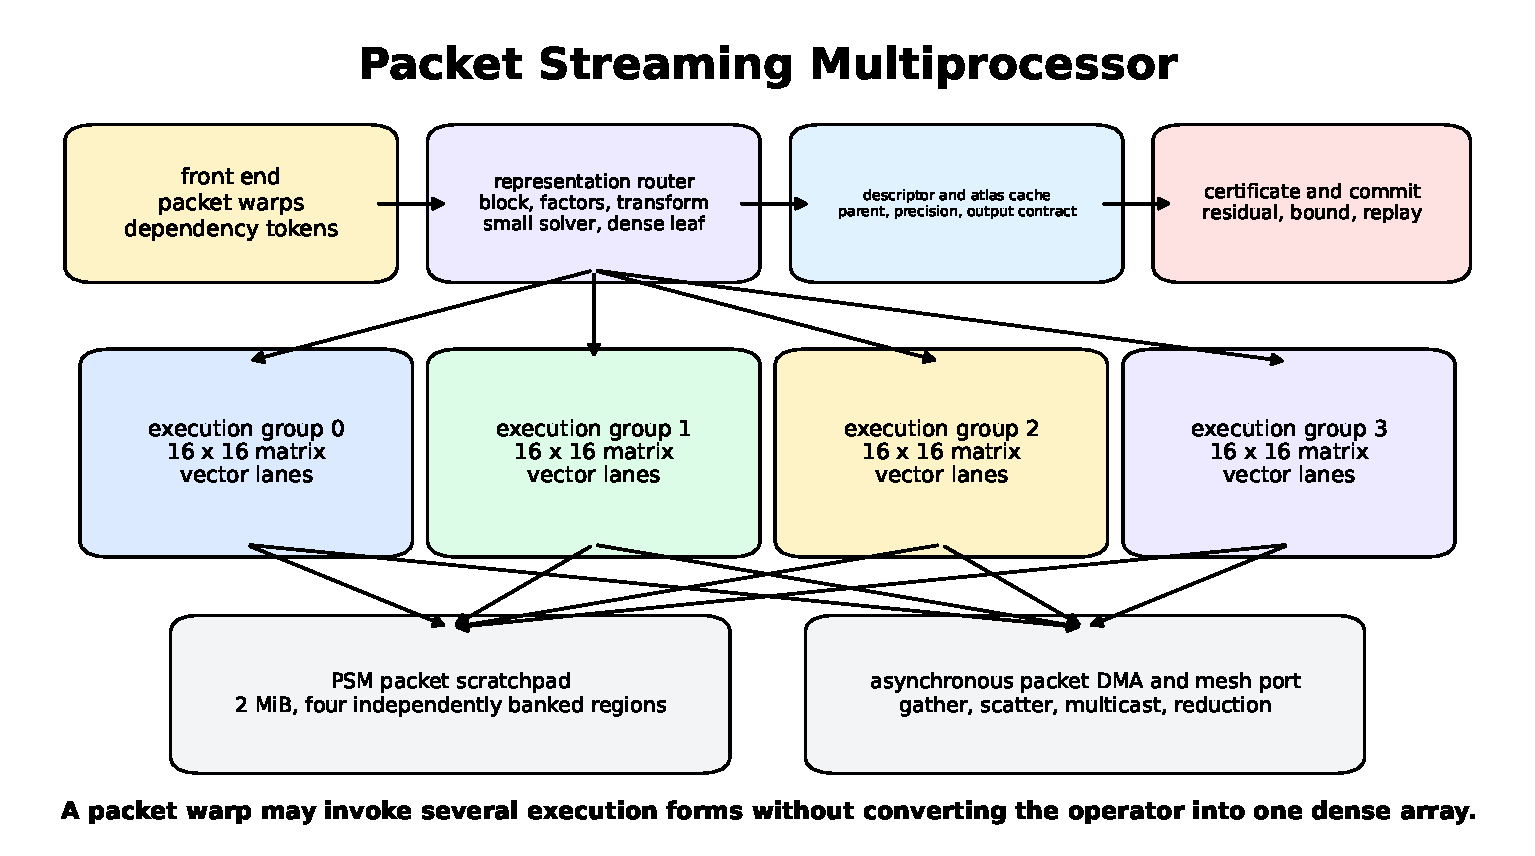
\includegraphics[width=0.98\linewidth]{37_packet_streaming_multiprocessor.pdf}
\caption{One Packet Streaming Multiprocessor. A packet warp may use several execution forms without converting the operator into one explicit array.}
\end{figure}

\section{Issue and completion path}
A packet warp becomes ready when its dependency token is satisfied and the packet directory confirms that the source representation is resident or in flight. The front end selects the representation route, reserves destination storage, and records the required certificate. Kernel completion produces a provisional result. The result becomes visible only after the check passes.

\begin{figure}[H]
\centering
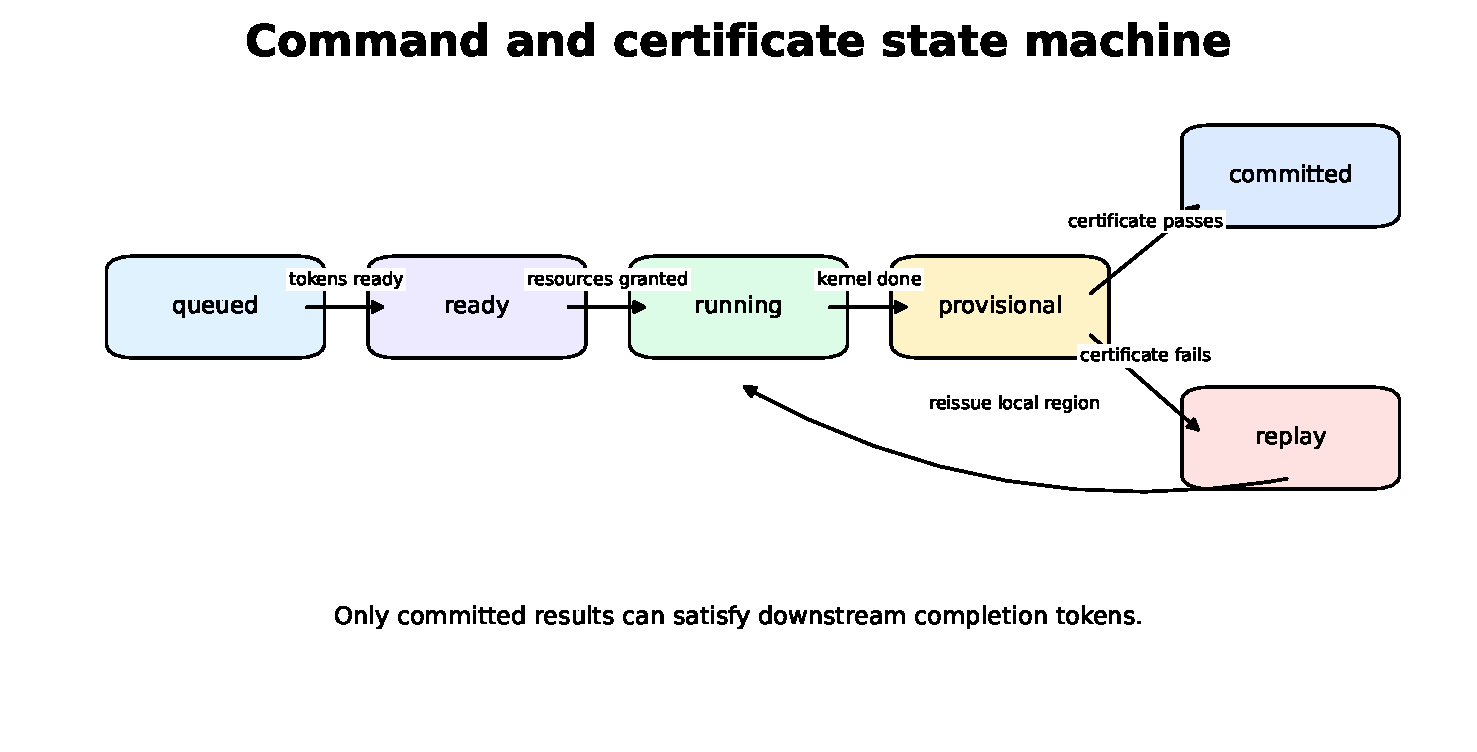
\includegraphics[width=0.90\linewidth]{28_command_state_machine.pdf}
\caption{Command states from queue entry to commit or local replay.}
\end{figure}

Completion and commitment remain separate. A kernel may finish while its residual exceeds the declared budget. The distinction matters for mixed precision, iterative solves, approximate transforms, recovered edge packets, and low-rank recompression.

\section{Packet scratchpad}
Each multiprocessor has 2 MiB of scratchpad divided into four independently banked regions. An execution group may use one bank privately or several groups may share a packet region. Separate banks hold active data, factors, descriptors, tokens, solver panels, and certificate state. Double buffering supports transforms and repeated grouped matrix batches.

\section{Execution groups}
Each of the four execution groups contains a $16\times16$ matrix array and programmable vector lanes. Equal-shape blocks can be grouped across execution groups. The same lanes handle low-rank contractions, Kronecker mode products, sparse-chain factors, selectors, reductions, index generation, and generic leaves.

Complex arithmetic uses paired real lanes. FP64 is available for certificates, small solvers, rank decisions, phase recovery, and sensitive reductions. Integer and fixed-point modes support selectors, image packets, modular arithmetic, and exact accumulators.

\begin{figure}[H]
\centering
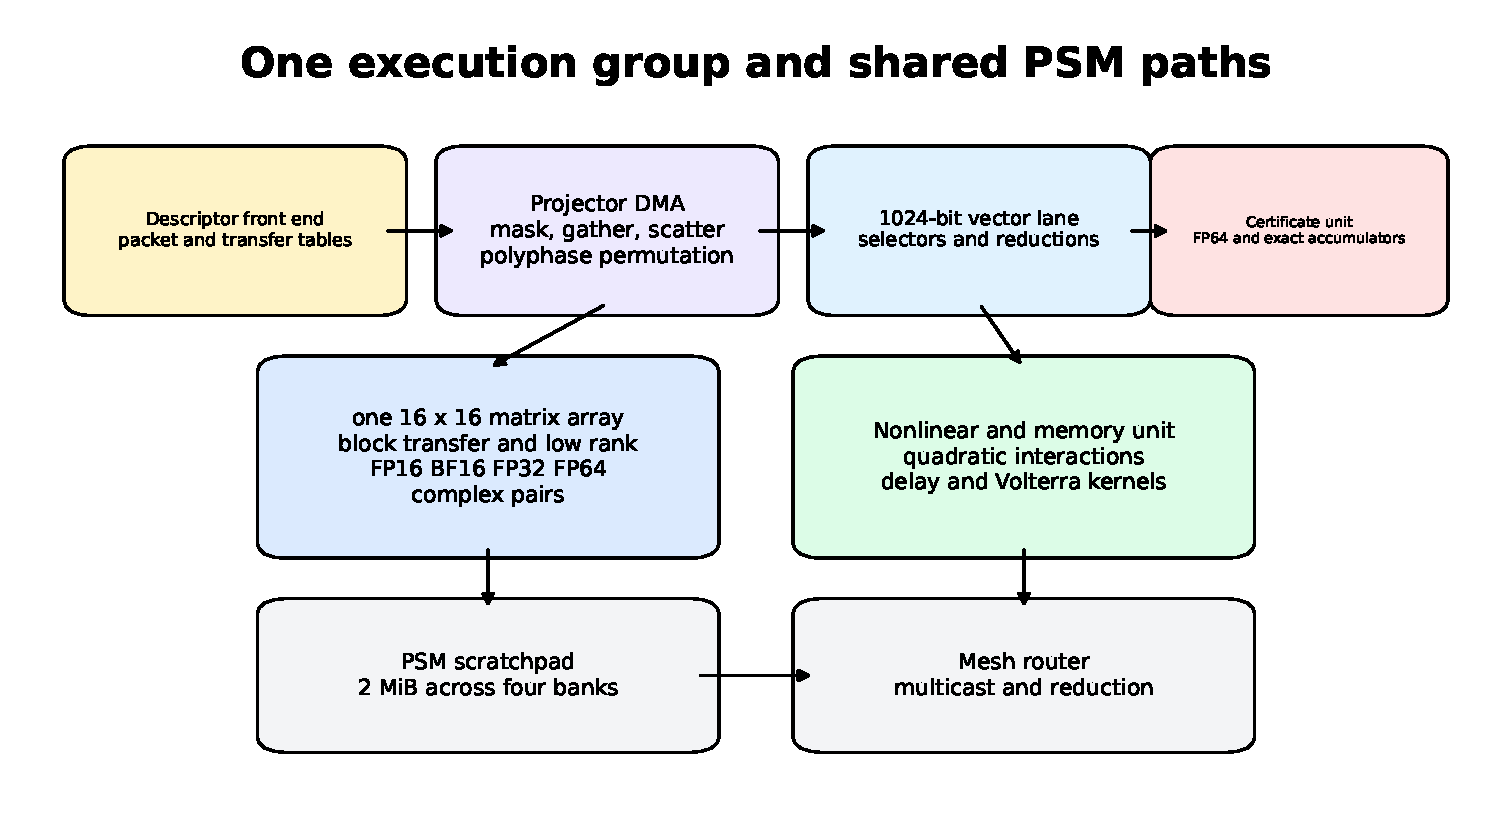
\includegraphics[width=0.93\linewidth]{02_packet_compute_tile.pdf}
\caption{Execution-group resources inside the multiprocessor. The figure shows matrix, vector, memory, nonlinear, and certificate paths.}
\end{figure}

\section{Representation router}
The router reads the operator form from Packet IR. It dispatches block work to grouped matrix lanes, factor work to contraction lanes, transform plans to the transform fabric, small algebraic systems to resident solvers, and weakly structured leaves to the generic path. One packet warp may contain several representations.

\section{Projector DMA}
The asynchronous packet DMA accepts selectors represented as intervals, strided slices, residue classes, polyphase channels, masks, index lists, transform bands, packet-tree nodes, and compact basis factors. A selector is applied through addressing and compact arithmetic. No dense projector matrix is required.

\section{Certificate and commit path}
The certificate unit accumulates residuals, packet norms, trace quantities, energy partitions, branch margins, and mixed-precision bounds. Deterministic mode uses a fixed reduction tree and wide accumulation. The commit controller releases a provisional result only after the declared acceptance rule passes.

\chapter{Descriptors as the hardware language}

\section{Packet descriptor entry}
A packet descriptor identifies the packet, its parent, its atlas, its selector, its shape, its location, its precision, and its error budget.

\begin{figure}[H]
\centering
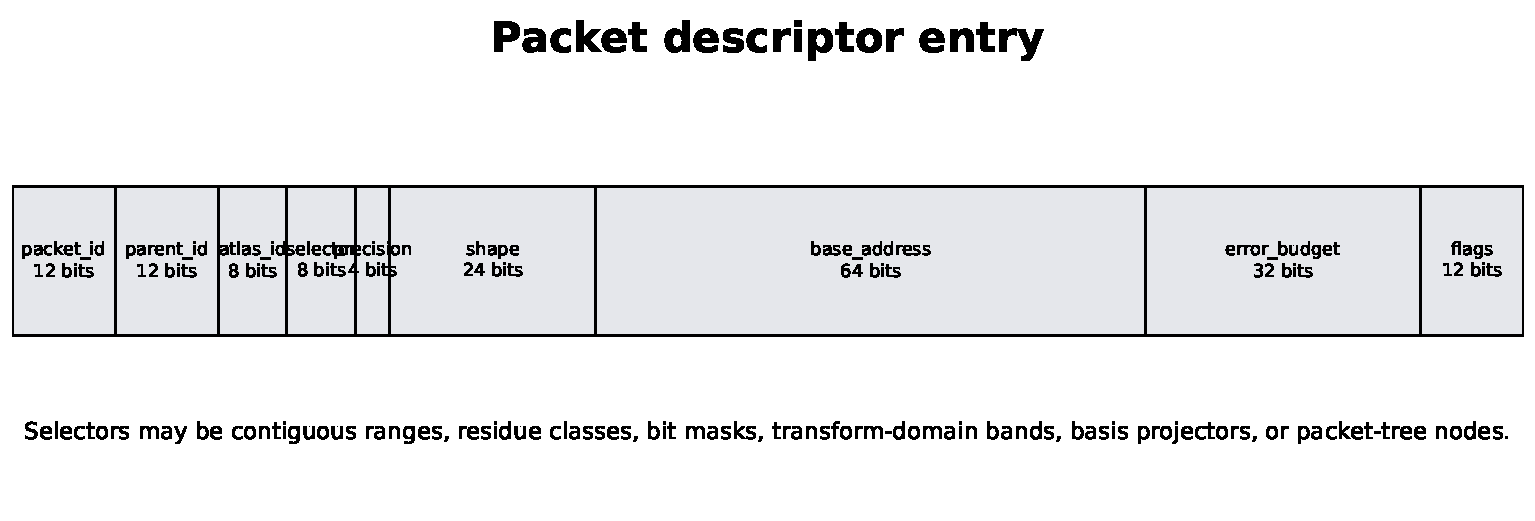
\includegraphics[width=0.98\linewidth]{04_packet_descriptor.pdf}
\caption{One packet descriptor entry. The exact bit allocation may change during RTL design, but the semantic fields are fixed.}
\end{figure}

\begin{definition}[Packet descriptor]
A packet descriptor is a typed record
\[
\mathsf P=(i,p,a,\sigma,\mathbf n,\ell,\pi,\tau),
\]
where $i$ is the packet ID, $p$ is the parent, $a$ is the atlas, $\sigma$ is the selector type, $\mathbf n$ is the shape, $\ell$ is the storage location, $\pi$ is the precision tag, and $\tau$ is the allowed local error contribution.
\end{definition}

\section{Transfer edge descriptor}
The transfer descriptor is the hardware form of $P_\beta T P_\alpha$. It identifies the source and destination packets, operator class, shape, rank, precision, sensitivity, payload, and dependency token.

\begin{figure}[H]
\centering
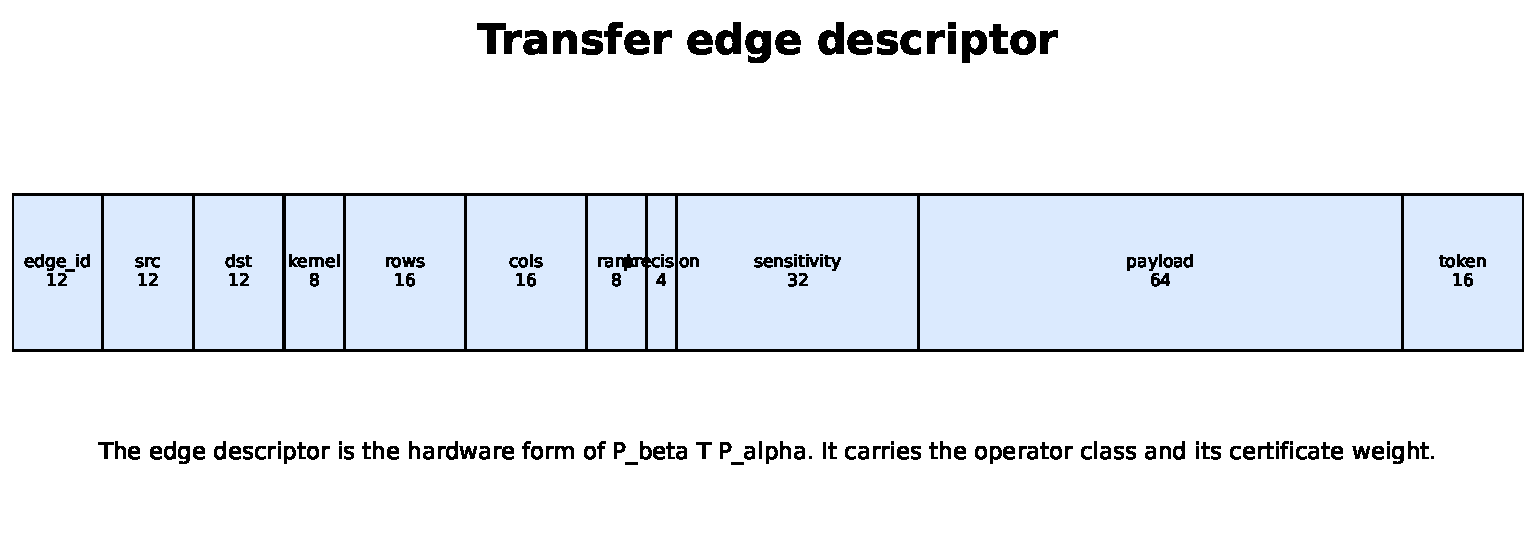
\includegraphics[width=0.98\linewidth]{05_transfer_descriptor.pdf}
\caption{A transfer edge descriptor keeps the operator class and certificate weight attached to the edge.}
\end{figure}

\section{Atlas descriptor}
An atlas descriptor records an analysis graph, a synthesis graph, normalization data, and packet selectors. A unitary transform uses its adjoint for synthesis. A redundant exact frame records the canonical dual or another declared synthesis map satisfying
\[
\Scal\Acal=I.
\]

\chapter{Memory hierarchy}

\section{Exact archive and active representations}
The exact archive, cold factors, large graphs, and model history remain in HBM. Completeness does not imply a dense array. An exact archive may be a transform tuple, factor graph, sparse chain, packet tree, geometric edge list, or explicit sample field. Shared SRAM stores active packet graphs and reusable representations. PSM scratchpads hold local blocks, factor panels, transform stages, solver panels, and residuals.

\begin{figure}[H]
\centering
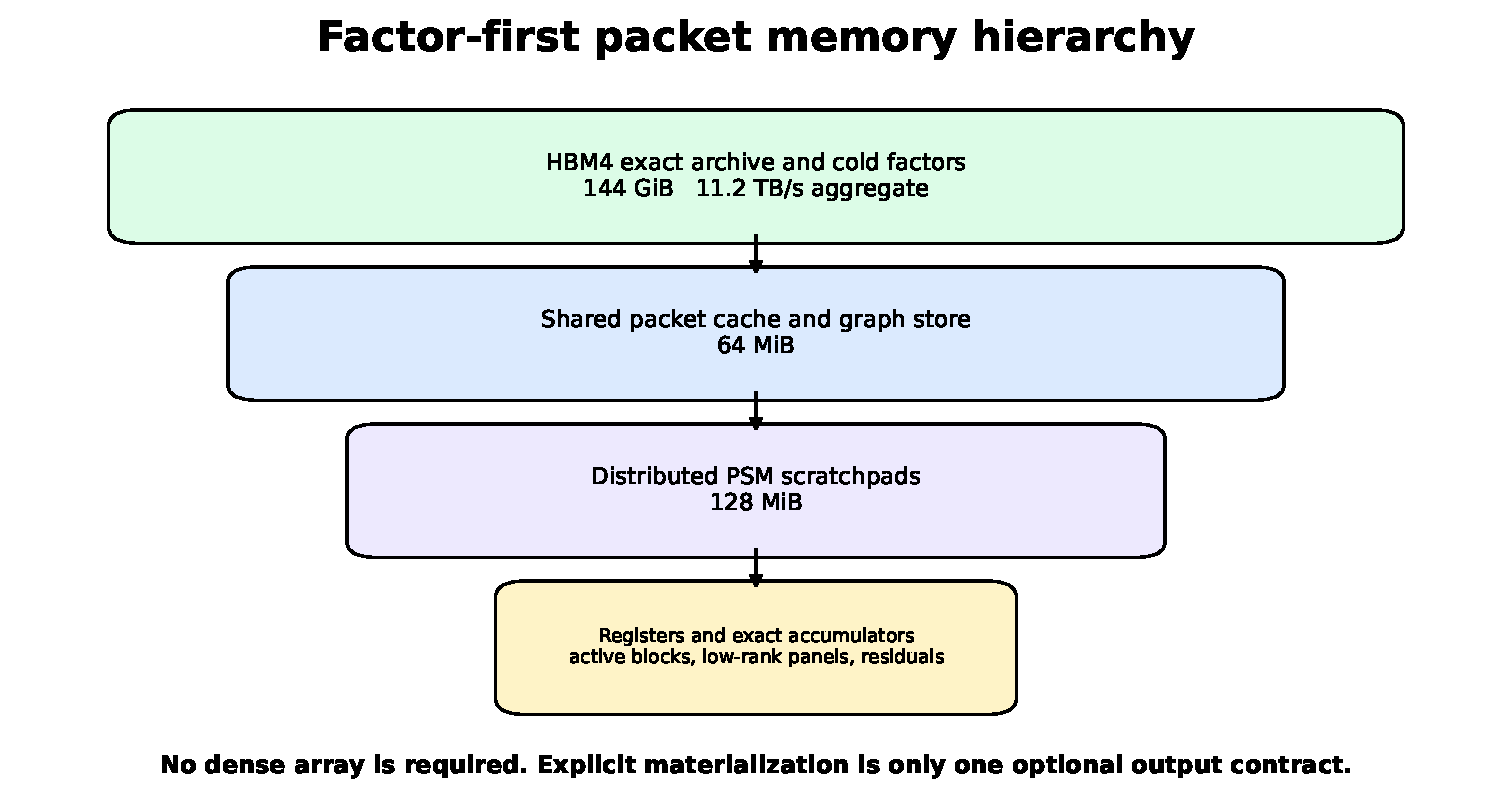
\includegraphics[width=0.90\linewidth]{06_memory_hierarchy.pdf}
\caption{Representation-first memory hierarchy. The explicit full array is created only under a matching output contract.}
\end{figure}

\section{Representation-first storage}
For an equal-block BDLR operator
\[
A=D+UV^*,
\]
with dimension $n$, block width $b$, and rank $r$, the stored scalar count is
\[
\boxed{n(b+2r)}
\]
in place of $n^2$.

\begin{proposition}[BDLR representation reduction]
If $b+2r<n$, BDLR storage reduces the scalar count by
\[
\boxed{\frac{n}{b+2r}.}
\]
The same factor appears in the ideal apply count for a fixed number of right-hand sides.
\end{proposition}

\begin{proof}
The block-diagonal part stores $(n/b)b^2=nb$ scalars. The two rank factors store $2nr$. The total is $n(b+2r)$. A full array stores $n^2$ scalars.
\end{proof}

The same rule extends beyond BDLR. A Kronecker operator stores its mode factors. A butterfly stores its sparse stages. A transform-domain operator stores the plan and diagonal or block payload. A packet graph stores packet descriptors and active edge payloads. The active representation is the operator until a different output contract is requested.

\begin{figure}[H]
\centering
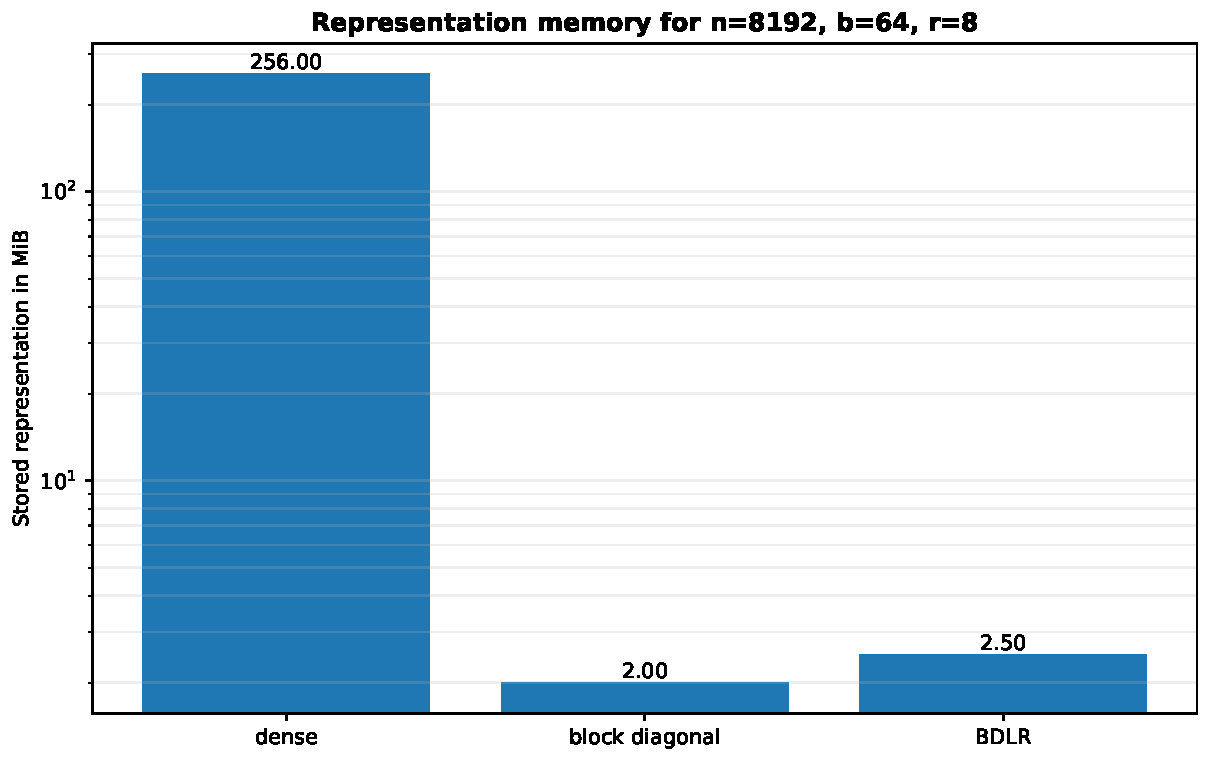
\includegraphics[width=0.76\linewidth]{16_representation_memory.pdf}
\caption{Stored BDLR representation for the model case $n=8192$, $b=64$, and $r=8$.}
\end{figure}

\chapter{Packet network and scheduling}

\section{PSM mesh}
Each compute chiplet uses a $4\times4$ mesh of Packet Streaming Multiprocessors. Routers support unicast, multicast, and tree reduction. Multicast distributes low-rank factors, Kronecker factors, and transform data. Reduction combines destination contributions, small contractions, posterior scores, and residuals.

\begin{figure}[H]
\centering
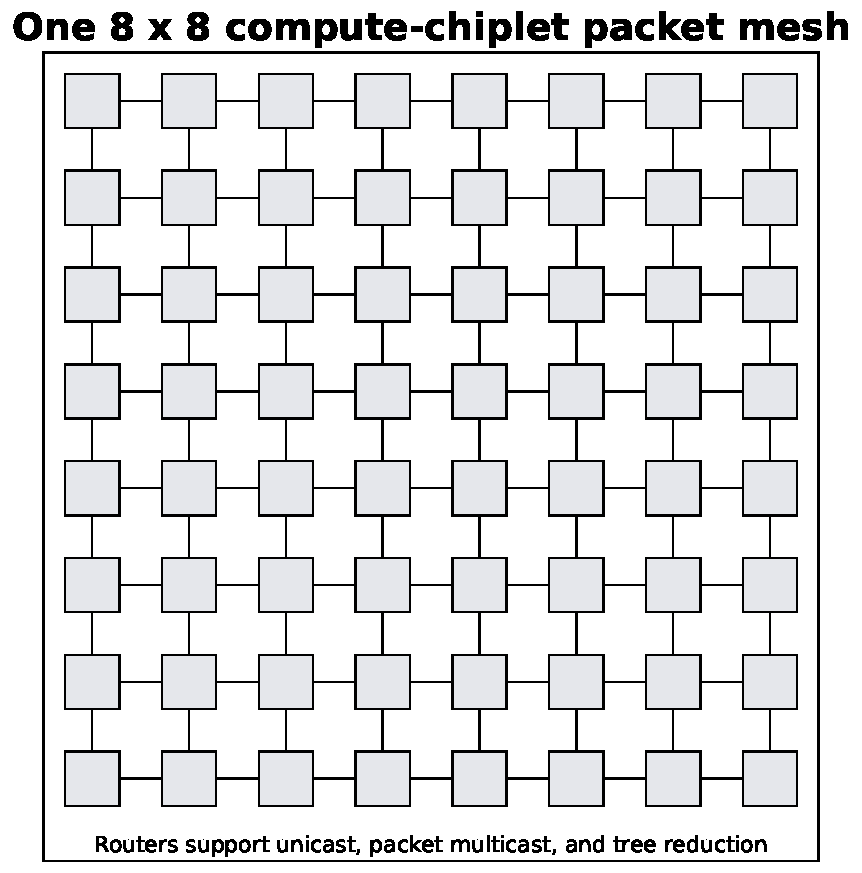
\includegraphics[width=0.62\linewidth]{20_packet_mesh.pdf}
\caption{One chiplet mesh. Each displayed router node represents one Packet Streaming Multiprocessor rather than one execution group.}
\end{figure}

\section{Packet warps and dependency tokens}
Packet warps group operations that share a representation, shape class, packet relation, or certificate boundary. A warp becomes ready when its dependency tokens are satisfied. Completion tokens wake downstream work. Replayable regions keep descriptors and placement until a certificate mismatch or local refinement invalidates the region.

\section{Local refinement}
Suppose a parent packet task $v$ is replaced by an acyclic child module $H=(W,F)$. Predecessors of $v$ connect to child entries. Child exits connect to successors of $v$.

\begin{theorem}[Topological splice]
Let $\prec$ be a topological order of the original graph and let $\prec_H$ be a topological order of the child module. Replacing $v$ in $\prec$ by $\prec_H$ gives a topological order of the refined graph. Every unaffected pair of context tasks keeps its relative order.
\end{theorem}

\begin{proof}
Every context edge is unchanged. Every child edge is respected by $\prec_H$. Every predecessor of $v$ appeared before $v$ and therefore before the inserted child order. Every successor appeared after $v$ and therefore after the inserted child order. Removing the inserted children restores the original context order.
\end{proof}

\begin{figure}[H]
\centering
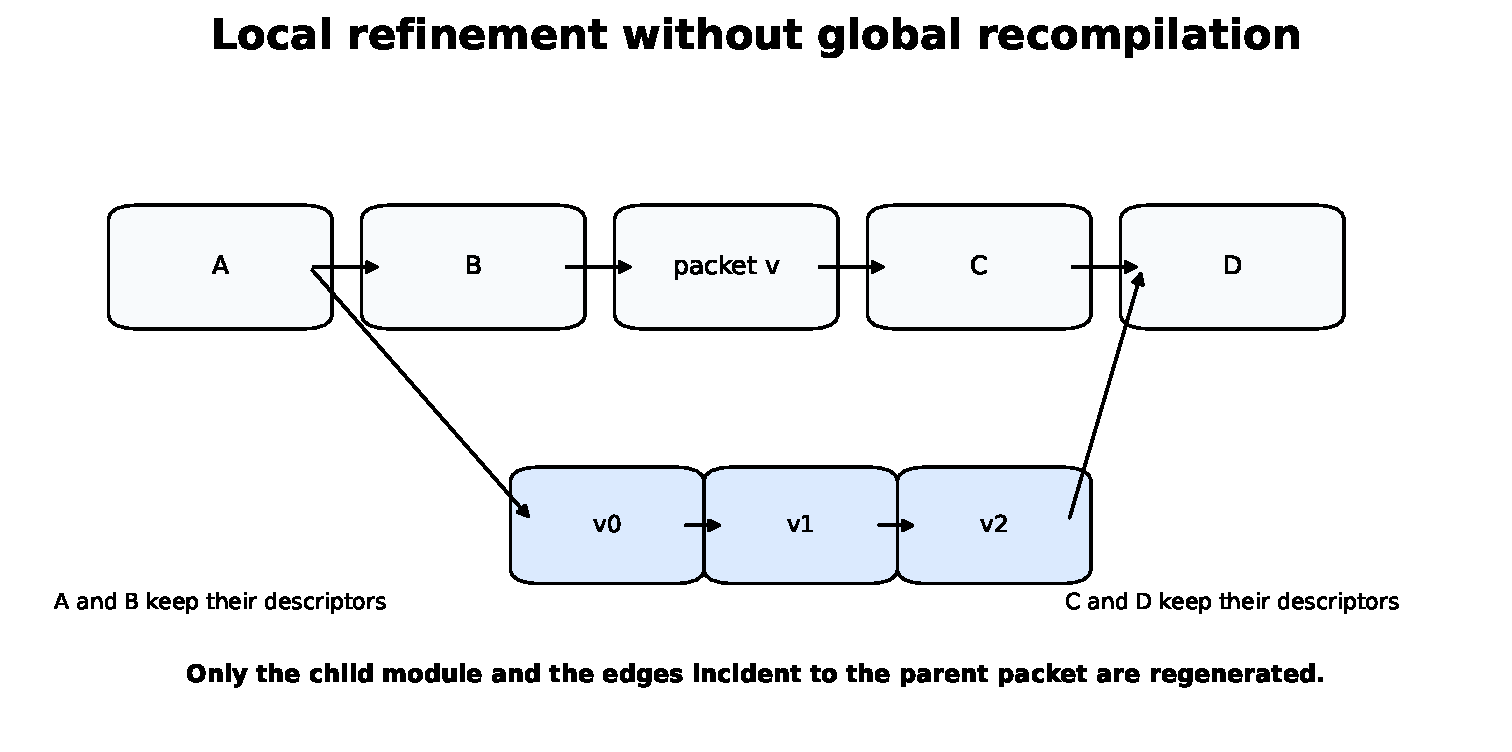
\includegraphics[width=0.74\linewidth]{11_refinement_local_schedule.pdf}
\caption{A parent packet is replaced by a local child graph while remote descriptors remain unchanged.}
\end{figure}

\chapter{Transform fabric}

\section{One configurable engine family}
The transform engines share butterfly, permutation, lifting, and selector hardware. They support FFT, DCT, FWHT, Haar, biorthogonal lifting, and polyphase transforms.

\begin{figure}[H]
\centering
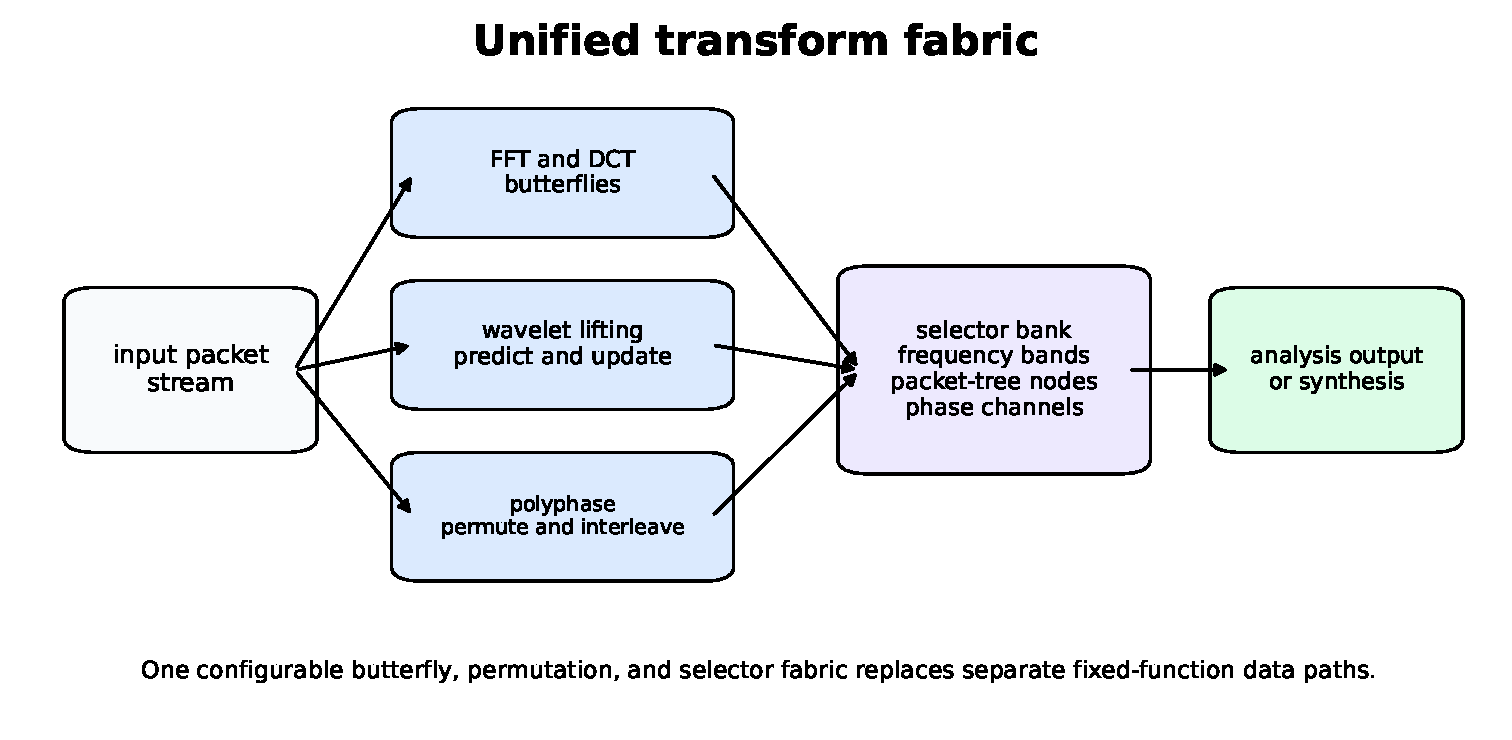
\includegraphics[width=0.92\linewidth]{08_transform_fabric.pdf}
\caption{The transform fabric supports several exact atlases without storing separate fixed data paths for each one.}
\end{figure}

\section{Exact analysis and synthesis}
Let $U$ be unitary and let $E_\alpha$ be coordinate selectors. The pulled-back projectors are
\[
P_\alpha=U^*E_\alpha U.
\]
The hardware analysis applies $U$ and selects the coordinates. Synthesis scatters the selected coordinates and applies $U^*$.

\begin{theorem}[Transform-atlas hardware contract]
If the selector family is complete, the analysis and synthesis command graphs satisfy
\[
\boxed{\Scal\Acal=I.}
\]
If the selector family is incomplete, the certificate must report the omitted-coordinate residual.
\end{theorem}

\begin{proof}
For a complete selector family, $\sum_\alpha E_\alpha=I$. Hence
\[
\Scal\Acal x
=U^*\left(\sum_\alpha E_\alpha\right)Ux
=U^*Ux
=x.
\]
The incomplete case replaces the identity by the declared selector sum.
\end{proof}

\chapter{Transfer engines}

\section{Block diagonal and block sparse}
Block-diagonal operators run as independent shape batches. Block-sparse operators are grouped by edge shape and destination. Destination packet accumulation can be local, multicast, or reduced through the mesh.

\section{BDLR dataflow}
For
\[
A=D+UV^*,
\]
the apply is
\[
AX=DX+U(V^*X).
\]
The diagonal blocks remain distributed. The $r\times q$ contraction is reduced and broadcast.

\begin{figure}[H]
\centering
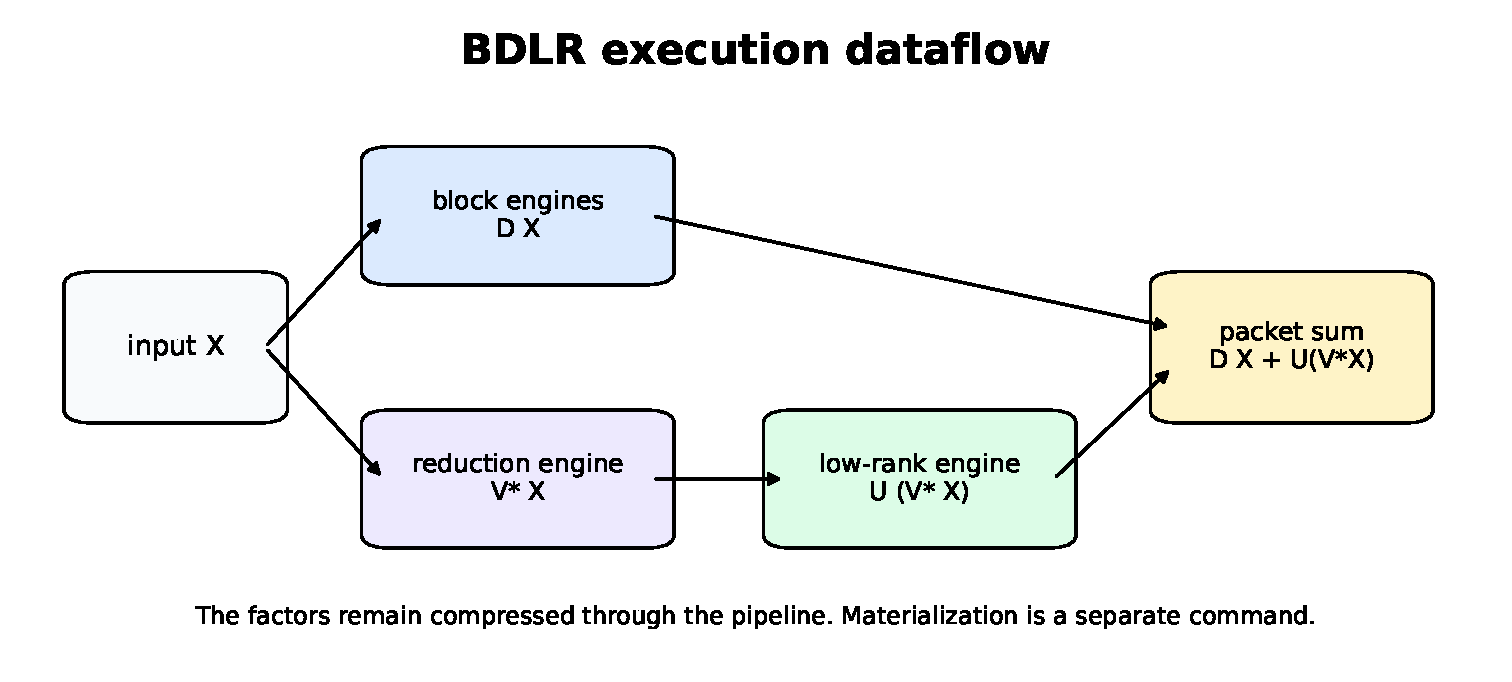
\includegraphics[width=0.92\linewidth]{07_bdlr_dataflow.pdf}
\caption{The BDLR path keeps the low-rank representation compressed.}
\end{figure}

\begin{theorem}[BDLR apply count]
For $q$ right-hand sides and equal packet width $b$, the modeled arithmetic count is
\[
\boxed{2qn(b+2r).}
\]
A dense apply requires $2qn^2$ operations.
\end{theorem}

\begin{proof}
The block-diagonal product costs $2qnb$. The contraction $V^*X$ costs $2nrq$. Multiplication by $U$ costs another $2nrq$. Adding the terms does not change the leading expression.
\end{proof}

\section{Where BDLR remains useful}
The low-rank path is not uniformly favorable. Its benefit depends on block width, correction rank, right-hand-side count, and factor reuse. The reference model sweeps a range of block sizes and ranks while holding $n=8192$ and $q=32$ fixed.

\begin{figure}[H]
\centering
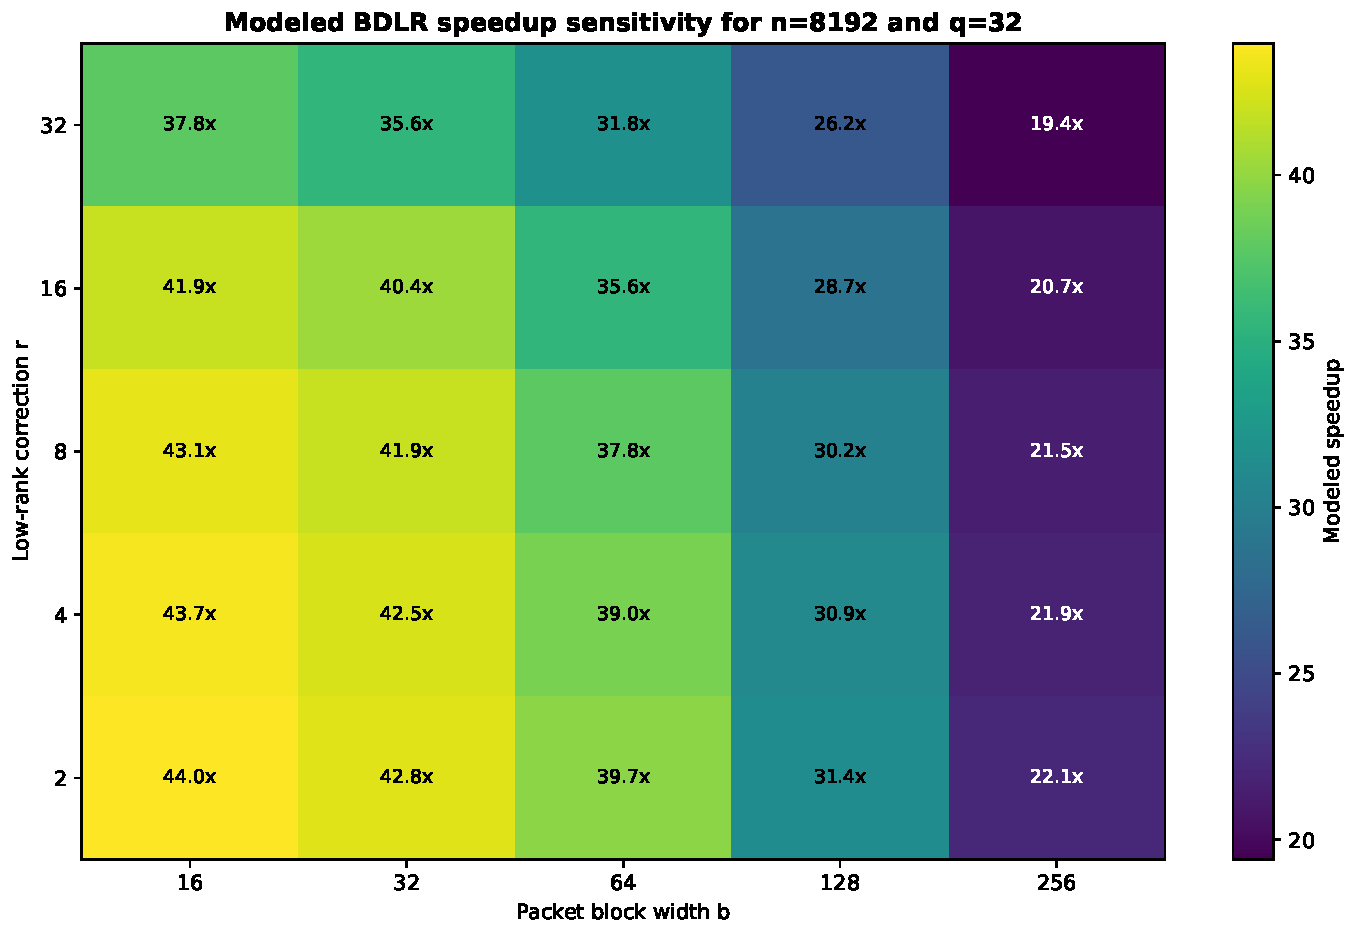
\includegraphics[width=0.82\linewidth]{29_bdlr_speedup_sensitivity.pdf}
\caption{Modeled BDLR speedup across block width and correction rank. The comparison includes arithmetic, data movement, and graph overhead from the reference model.}
\end{figure}

\begin{figure}[H]
\centering
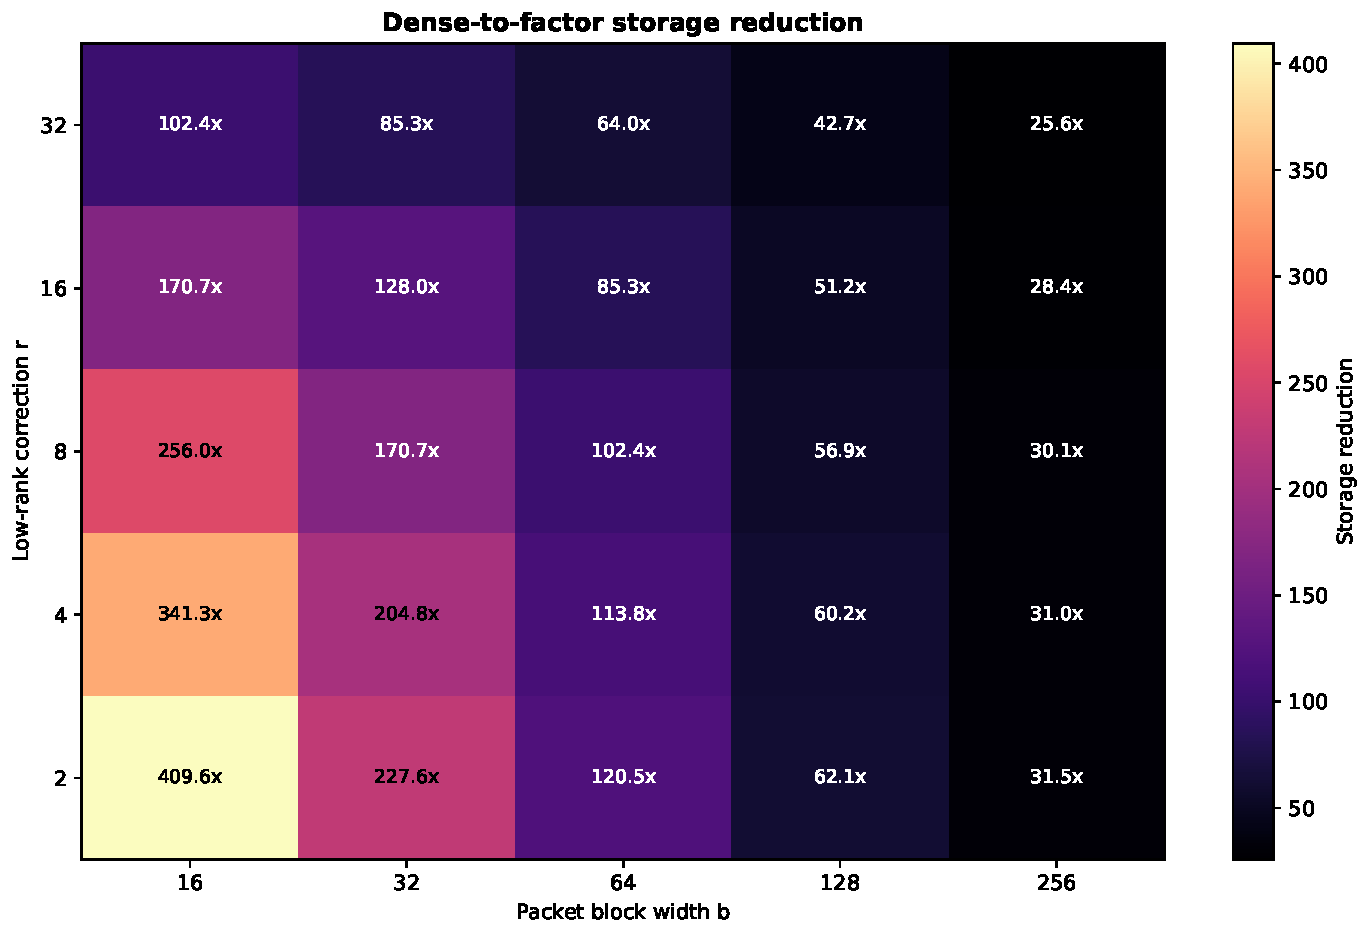
\includegraphics[width=0.82\linewidth]{30_bdlr_storage_sensitivity.pdf}
\caption{Dense-to-factor storage reduction for the same parameter sweep.}
\end{figure}

The compiler should not infer a gain from the name of the representation. It should evaluate the actual block width, rank, reuse, and output contract. A high-rank correction or a request for immediate dense materialization may remove most of the benefit.

\section{Compressed composition}
When downstream stages accept BDLR factors, composition returns new block factors and low-rank factors. Materialization is a separate output contract. The compiler cannot compare a compressed product with a dense explicit matrix without accounting for that difference.

\section{Woodbury solve}
The chip uses packet solves with $D_\alpha$ and one small dense correction:
\[
(D+UV^*)^{-1}
=D^{-1}-D^{-1}U(I+V^*D^{-1}U)^{-1}V^*D^{-1}.
\]
The solver engines handle the rank-sized middle system.

\chapter{Mixed precision and certificates}

\section{Per-edge precision}
A global dtype ignores the fact that packet transfers can have very different sensitivities. Each edge carries its precision and sensitivity.

\begin{theorem}[Packet error bound]
Let
\[
A=\sum_{e\in E}A_e,
\qquad
\widehat A=\sum_{e\in E}(A_e+E_e).
\]
If edge $e$ starts in packet $\alpha(e)$, then
\[
\boxed{
\norm{(\widehat A-A)x}
\le
\sum_{e\in E}\norm{E_e}\norm{P_{\alpha(e)}x}.}
\]
\end{theorem}

\begin{proof}
Exact packet reconstruction gives
\[
(\widehat A-A)x=\sum_eE_eP_{\alpha(e)}x.
\]
The triangle inequality gives the bound.
\end{proof}

\section{Precision allocation}
Under a logarithmic cost model and total error budget $\tau$, the continuous allocation is
\[
\varepsilon_e
=\frac{\tau c_e}{s_e\sum_f c_f},
\]
where $s_e$ is sensitivity and $c_e$ is cost. The compiler maps the result to supported formats.

\begin{figure}[H]
\centering
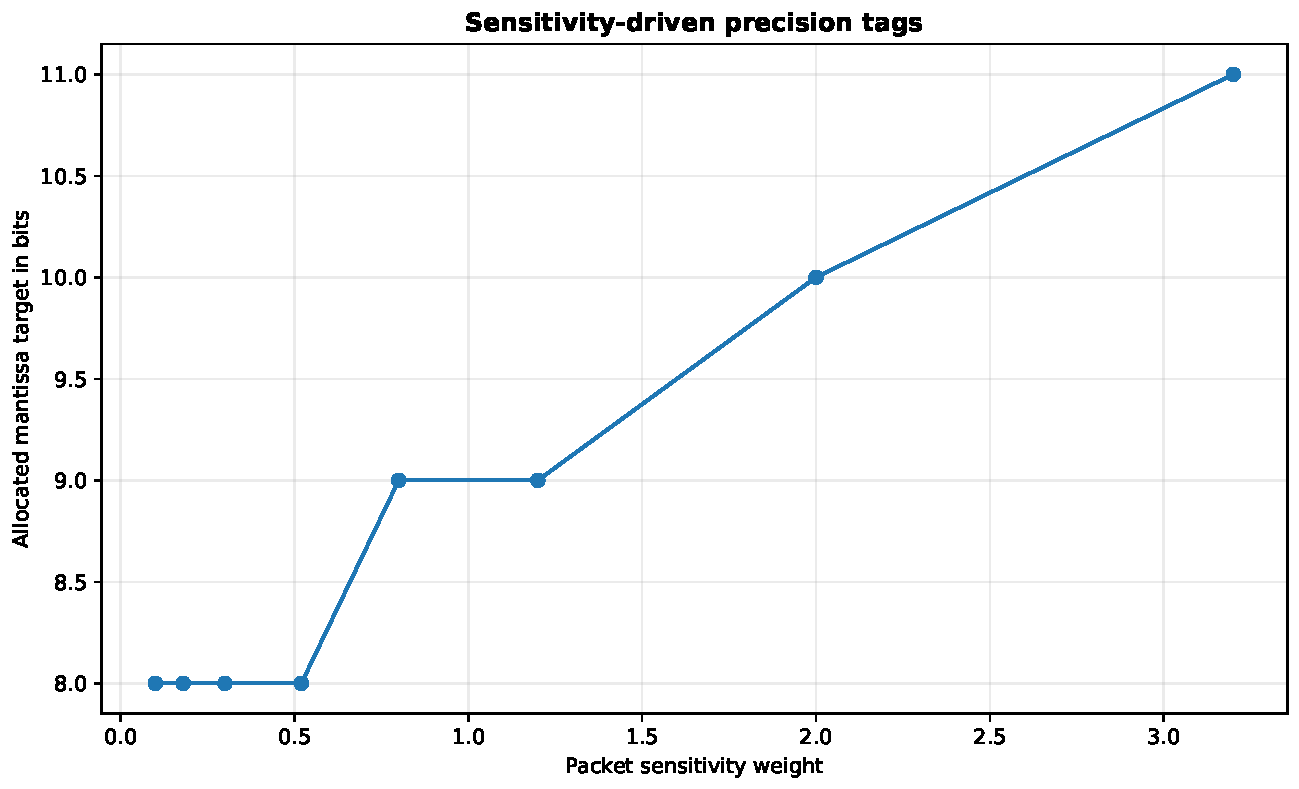
\includegraphics[width=0.78\linewidth]{19_precision_allocation.pdf}
\caption{More sensitive packet edges receive tighter precision targets.}
\end{figure}

\chapter{Unknown-edge and Gibbs reconstruction}

\section{Why the chip includes a small-solver path}
The self-calibrating reconstruction uses large transforms and very small algebraic systems in one graph. A general GPU often pays high launch and movement cost around the small systems. PRISM keeps the full chain resident.

\begin{figure}[H]
\centering
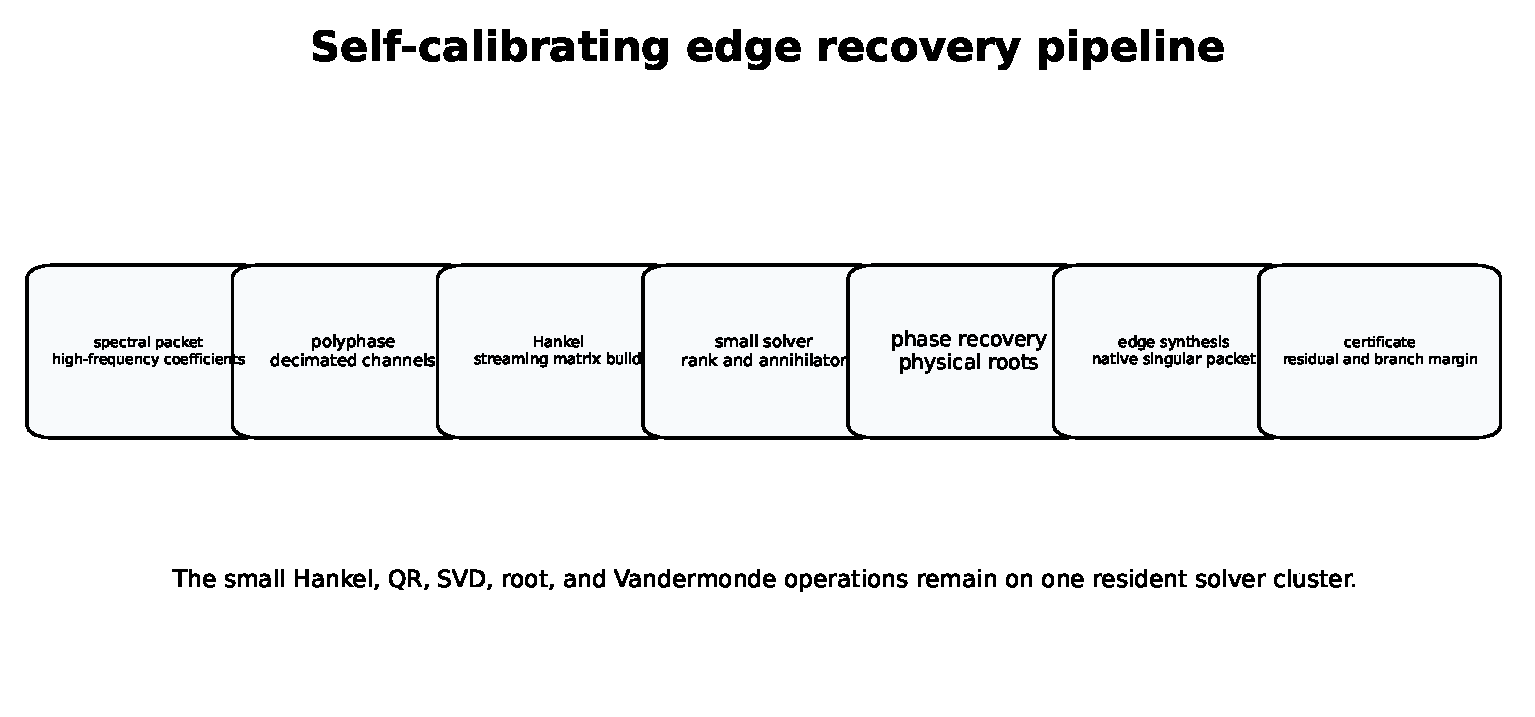
\includegraphics[width=0.98\linewidth]{09_edge_recovery_pipeline.pdf}
\caption{The self-calibrating edge-recovery graph from high-frequency packet to native singular synthesis.}
\end{figure}

\section{Resident Hankel and Prony operations}
The edge-recovery engines perform:
\begin{enumerate}
\item Fourier packet extraction
\item decimated polyphase grouping
\item streaming Hankel construction
\item rank estimation
\item annihilator solve
\item polynomial root recovery
\item physical phase selection
\item Vandermonde amplitude solve
\item edge packet synthesis
\item residual and branch-margin checks
\end{enumerate}

\section{Small-solver organization}
The solver cluster is built for matrices that are too small to fill the PSM mesh but too frequent to send back to the host. A local panel store feeds QR, Cholesky, Jacobi-style SVD, companion-matrix roots, and Vandermonde solves. FP64 is the default format for rank decisions, phase recovery, and branch-margin checks.

\begin{figure}[H]
\centering
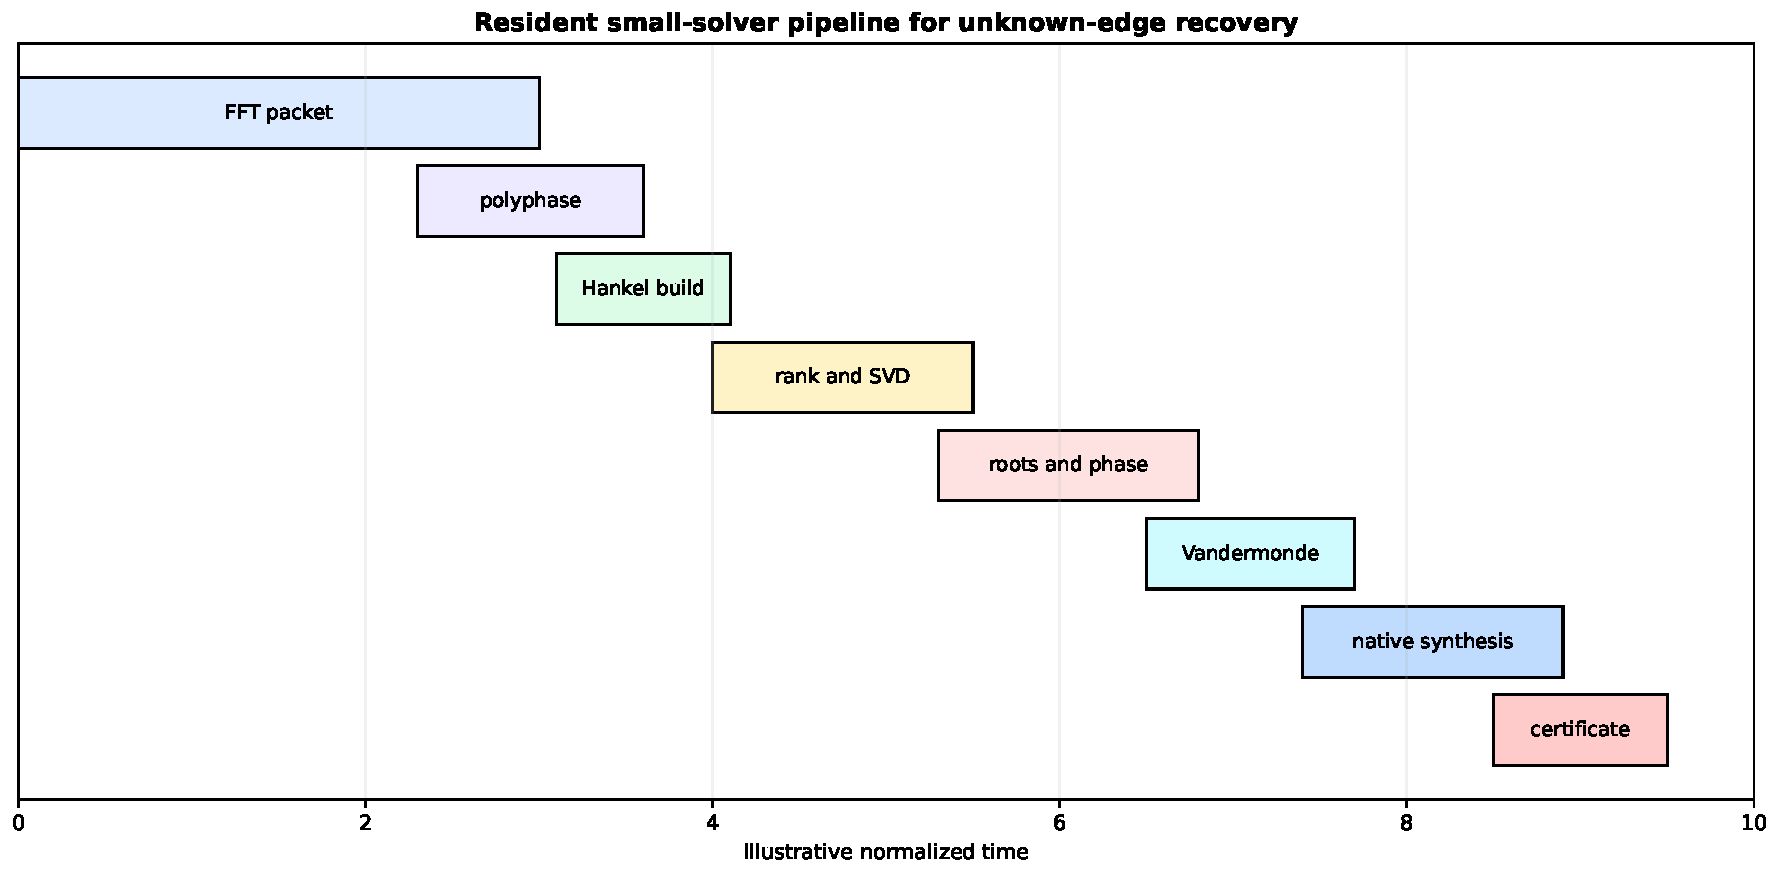
\includegraphics[width=0.92\linewidth]{31_solver_pipeline.pdf}
\caption{Illustrative resident pipeline for unknown-edge recovery. Transform and solver stages overlap where data dependencies permit.}
\end{figure}

The solver cluster is also used by Bayesian regression batches, Woodbury corrections, packet Krylov restarts, and small exactness checks. It is not intended to compete with a large dense eigensolver.

\section{Why native edge synthesis matters}
After edge recovery, the discontinuity is synthesized as an edge packet. The smooth residual is reconstructed spectrally. The chip does not force the recovered singular packet back through a truncated global Fourier sum.

\chapter{PR-LASM execution}

\section{Exact archive and compact state}
The exact observation archive is kept in complete spatial, Fourier, Haar, polyphase, and categorical atlases. Macro, meso, and micro states are separate statistical packet types with dimensions 48, 96, and 192 in the reference model.

\section{Resident state layout}
The exact archive and compact predictive states remain separate in memory and in the descriptor type system. This prevents a compact state vector from being mistaken for an invertible representation of the signal.

\begin{figure}[H]
\centering
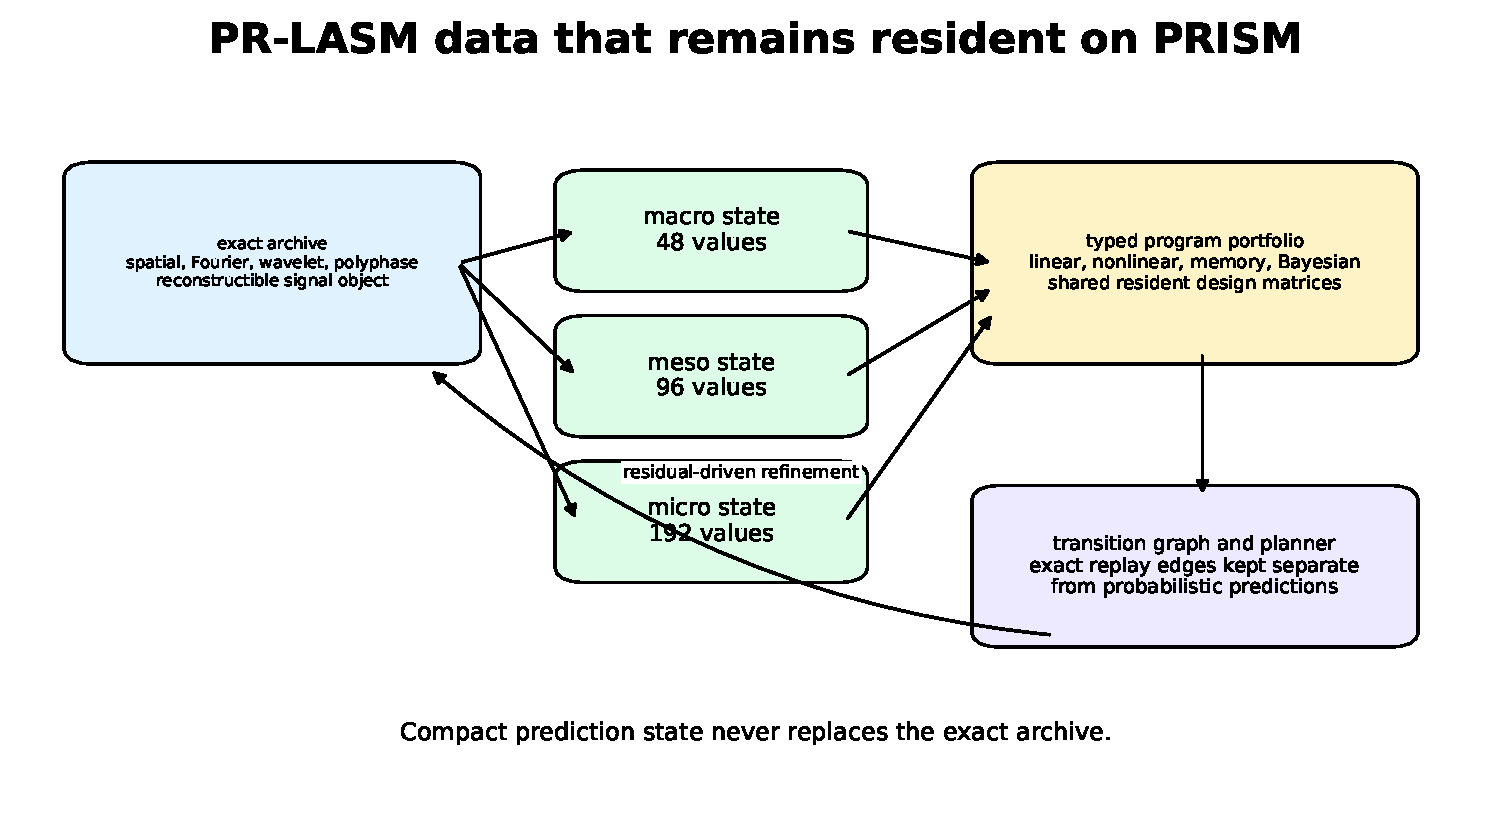
\includegraphics[width=0.96\linewidth]{32_pr_lasm_state_map.pdf}
\caption{Exact archive, compact states, mechanism portfolio, and transition graph in one resident PR-LASM step.}
\end{figure}

\section{Typed Bayesian programs}
The mechanism portfolio shares state matrices while allowing different operators, atlases, resolutions, and memory laws. The solver engines batch models by feature shape.

\begin{figure}[H]
\centering
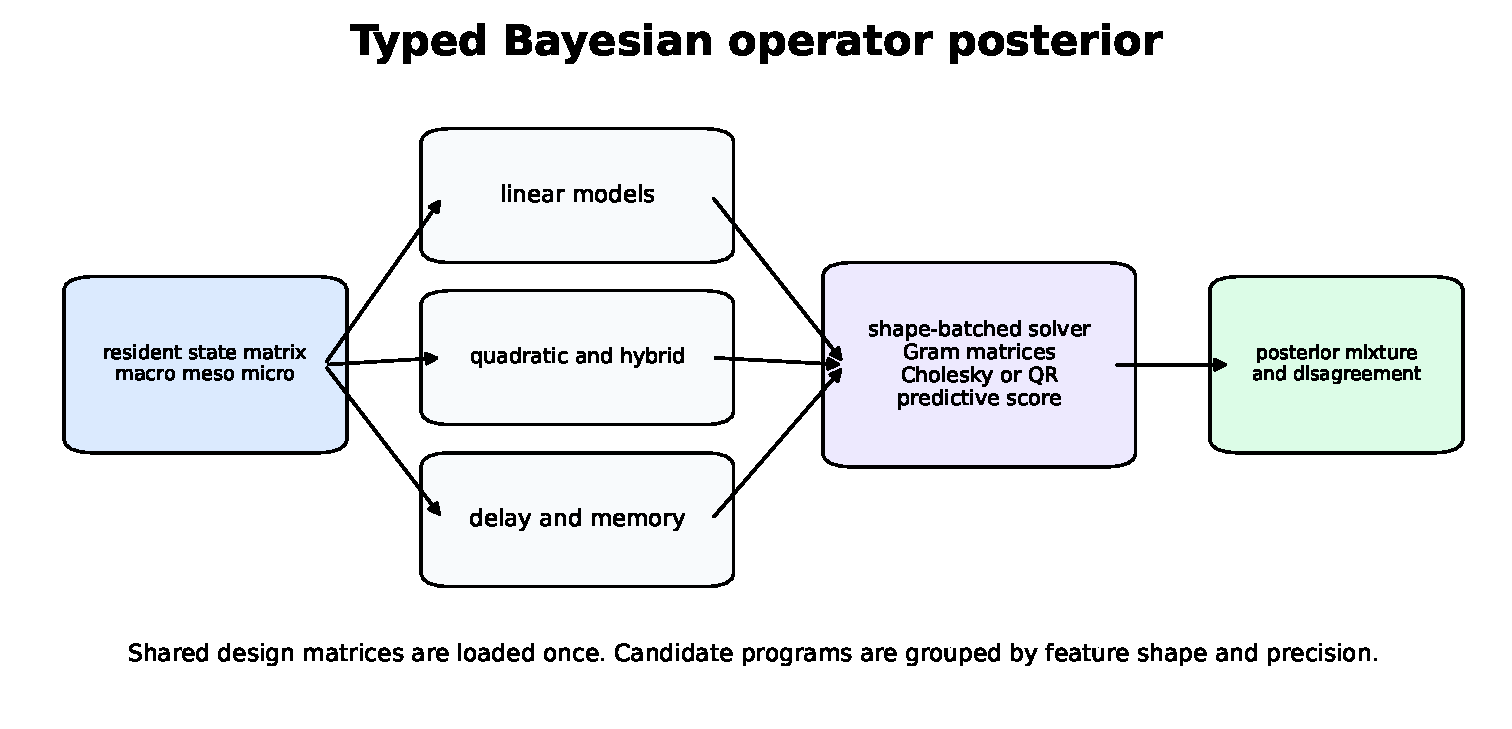
\includegraphics[width=0.92\linewidth]{10_bayesian_pipeline.pdf}
\caption{Mechanism families share resident state matrices and small-solver batches.}
\end{figure}

\section{Memory and planning}
Delay, power-law, exponential, and Volterra memory packets run in the nonlinear and memory units. The graph scheduler stores exact deterministic transitions separately from probabilistic predictions. Replay stops when a state or certificate mismatch is detected.

\chapter{Exact arithmetic mode}

\section{Residue and modular packets}
One exact arithmetic cluster per compute chiplet supports 64-bit modular addition, multiplication, valuation, residue selection, and CRT merge. Longer values use limb vectors in PSM scratchpad.

\section{Why this belongs on the chip}
The arithmetic calculus and the signal calculus share the same structural operations:
\[
\text{residue packet}
\to
\text{transfer}
\to
\text{refinement}
\to
\text{weighted reconstruction}.
\]
The exact arithmetic path is smaller than the floating-point path, but it allows the same descriptor and graph system to execute p-adic, recurrence, and finite-field packet workloads.

\chapter{Packet Seed Command interface}

\section{Command groups}
The first implementation uses memory-resident 256-bit commands. RISC-V control cores fill a queue and ring a doorbell. The command groups are shown below.

\begin{figure}[H]
\centering
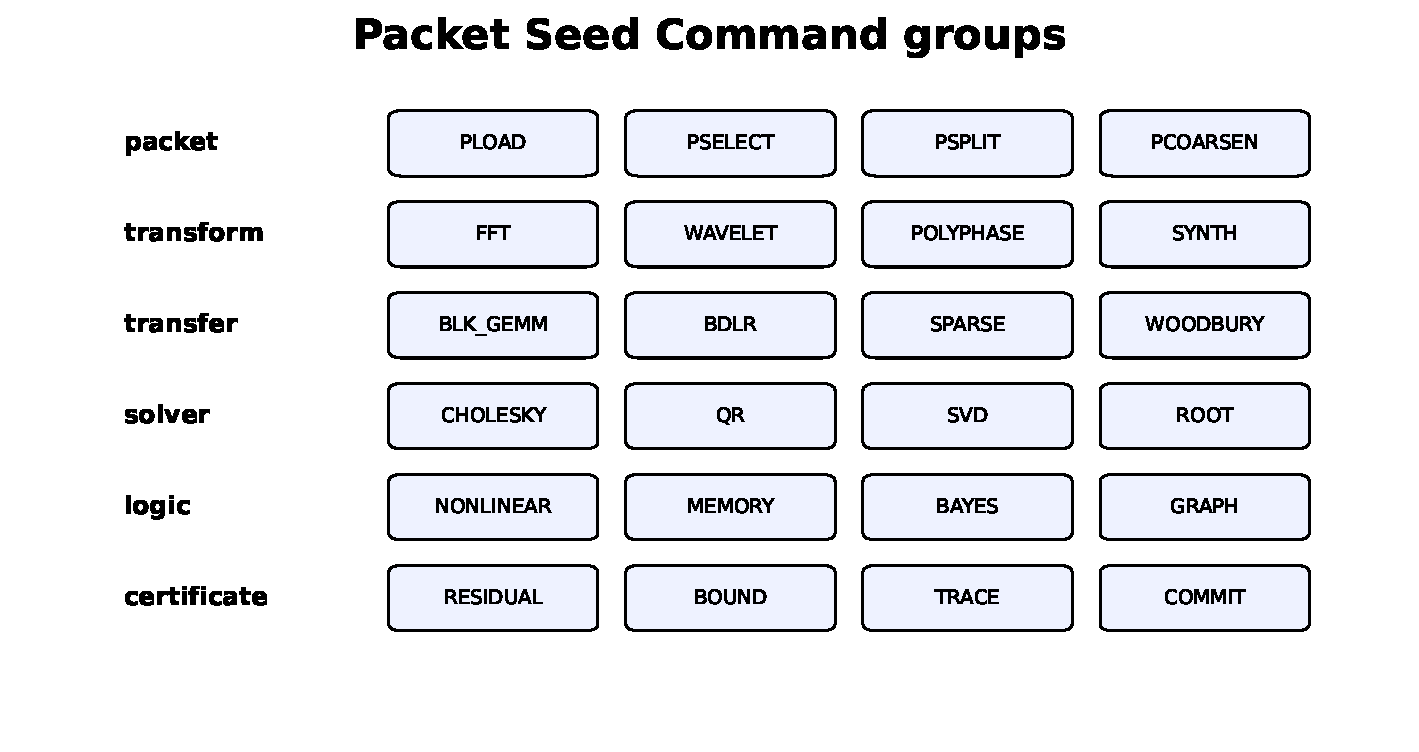
\includegraphics[width=0.92\linewidth]{21_command_groups.pdf}
\caption{Packet Seed Command groups.}
\end{figure}

\section{Representative commands}
\begin{longtable}{L{0.22\linewidth}L{0.68\linewidth}}
\toprule
Command & Meaning \\
\midrule
\endfirsthead
\toprule
Command & Meaning \\
\midrule
\endhead
\texttt{PSELECT} & Apply a declared packet selector without materializing a projector matrix \\
\texttt{PSPLIT} & Replace a parent packet by declared children \\
\texttt{PCOARSEN} & Reconstruct a parent from a complete child family \\
\texttt{POLYPHASE} & Extract, permute, or interleave phase channels \\
\texttt{WAVELET\_LIFT} & Execute predict, update, and scale steps \\
\texttt{BLK\_GEMM} & Execute a batch of equal-shape transfer blocks \\
\texttt{BDLR\_APPLY} & Apply block diagonal plus low rank without materialization \\
\texttt{HANKEL\_BUILD} & Stream moments into a small Hankel matrix \\
\texttt{ROOT\_PHASE} & Recover physical roots from decimated channels \\
\texttt{BAYES\_FIT} & Fit one shape-class batch of conjugate regressions \\
\texttt{GRAPH\_REFINE} & Replace one parent task by a local child graph \\
\texttt{RESIDUAL} & Form and store a reconstruction residual \\
\texttt{COMMIT} & Mark a result valid after required certificates pass \\
\bottomrule
\end{longtable}

\section{Completion record}
Every completed command produces a compact record containing the completion token, status, cycle count, bytes moved, exception code, residual summary, and certificate pointer. Downstream dependencies consume the token only after the commit state is reached.

\section{Protection and replay}
Descriptor tables, command queues, and certificate records require ECC or parity protection. A command that encounters an uncorrectable descriptor error is aborted before execution. A certificate failure invalidates only the declared replay region unless the error is marked package-wide.

\chapter{Compiler}

\section{Routing policy}
The compiler first asks whether the structure changes the cost of the computation. A named packet decomposition is not sufficient. The route decision uses representation size, expected reuse, graph size, materialization requirements, and measured or modeled engine cost.

\begin{figure}[H]
\centering
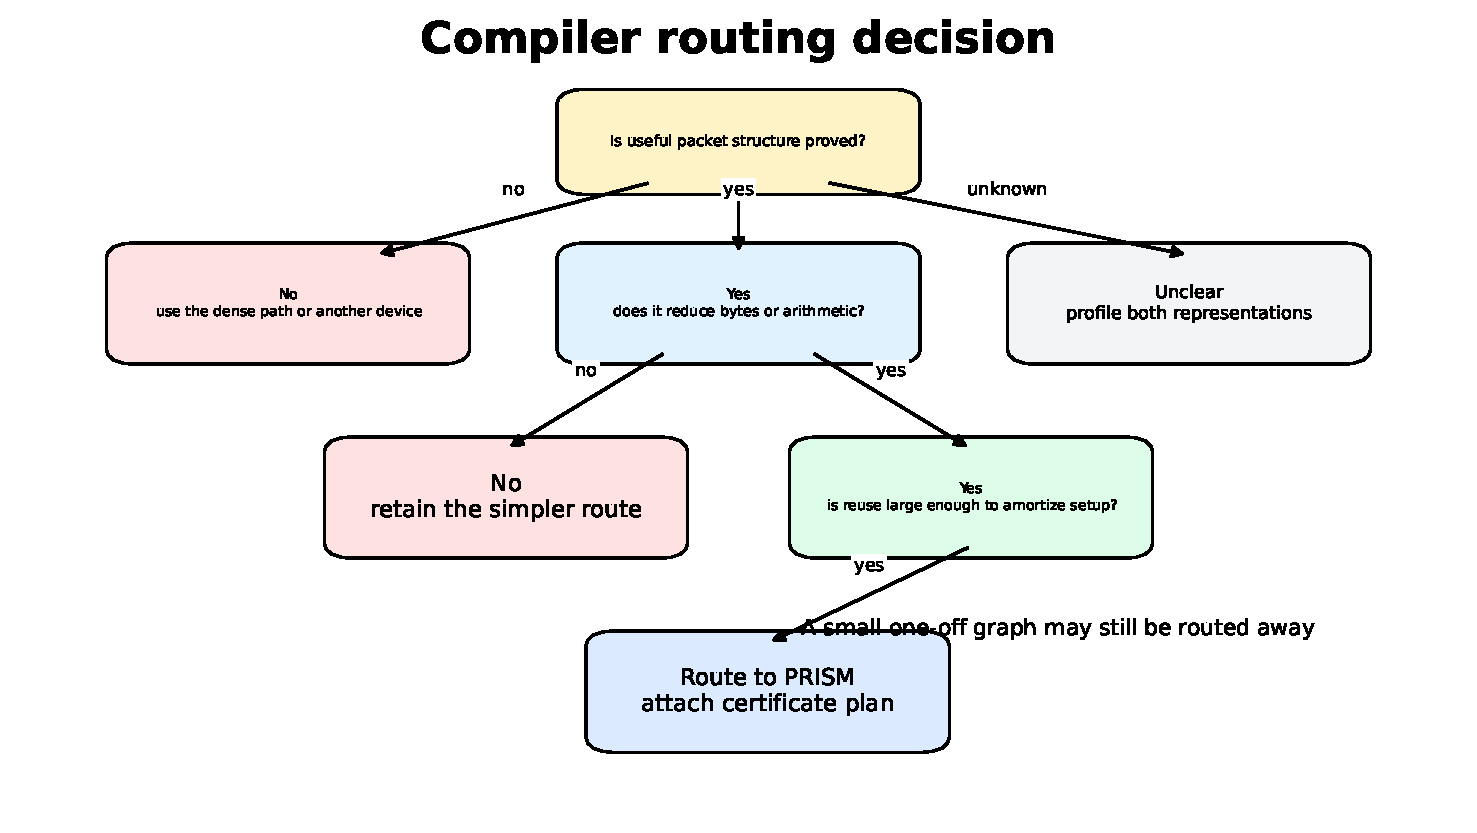
\includegraphics[width=0.88\linewidth]{25_workload_router.pdf}
\caption{Reference routing logic. The final compiler will use calibrated costs, but the reject path remains part of the specification.}
\end{figure}

\section{Shared Packet IR}
The CUDA and PRISM backends consume the same typed graph. Packet IR records representation form, packet and atlas identity, output contract, precision, reuse, dependencies, and certificate requirements. Backend selection does not change the mathematical result.

\begin{figure}[H]
\centering
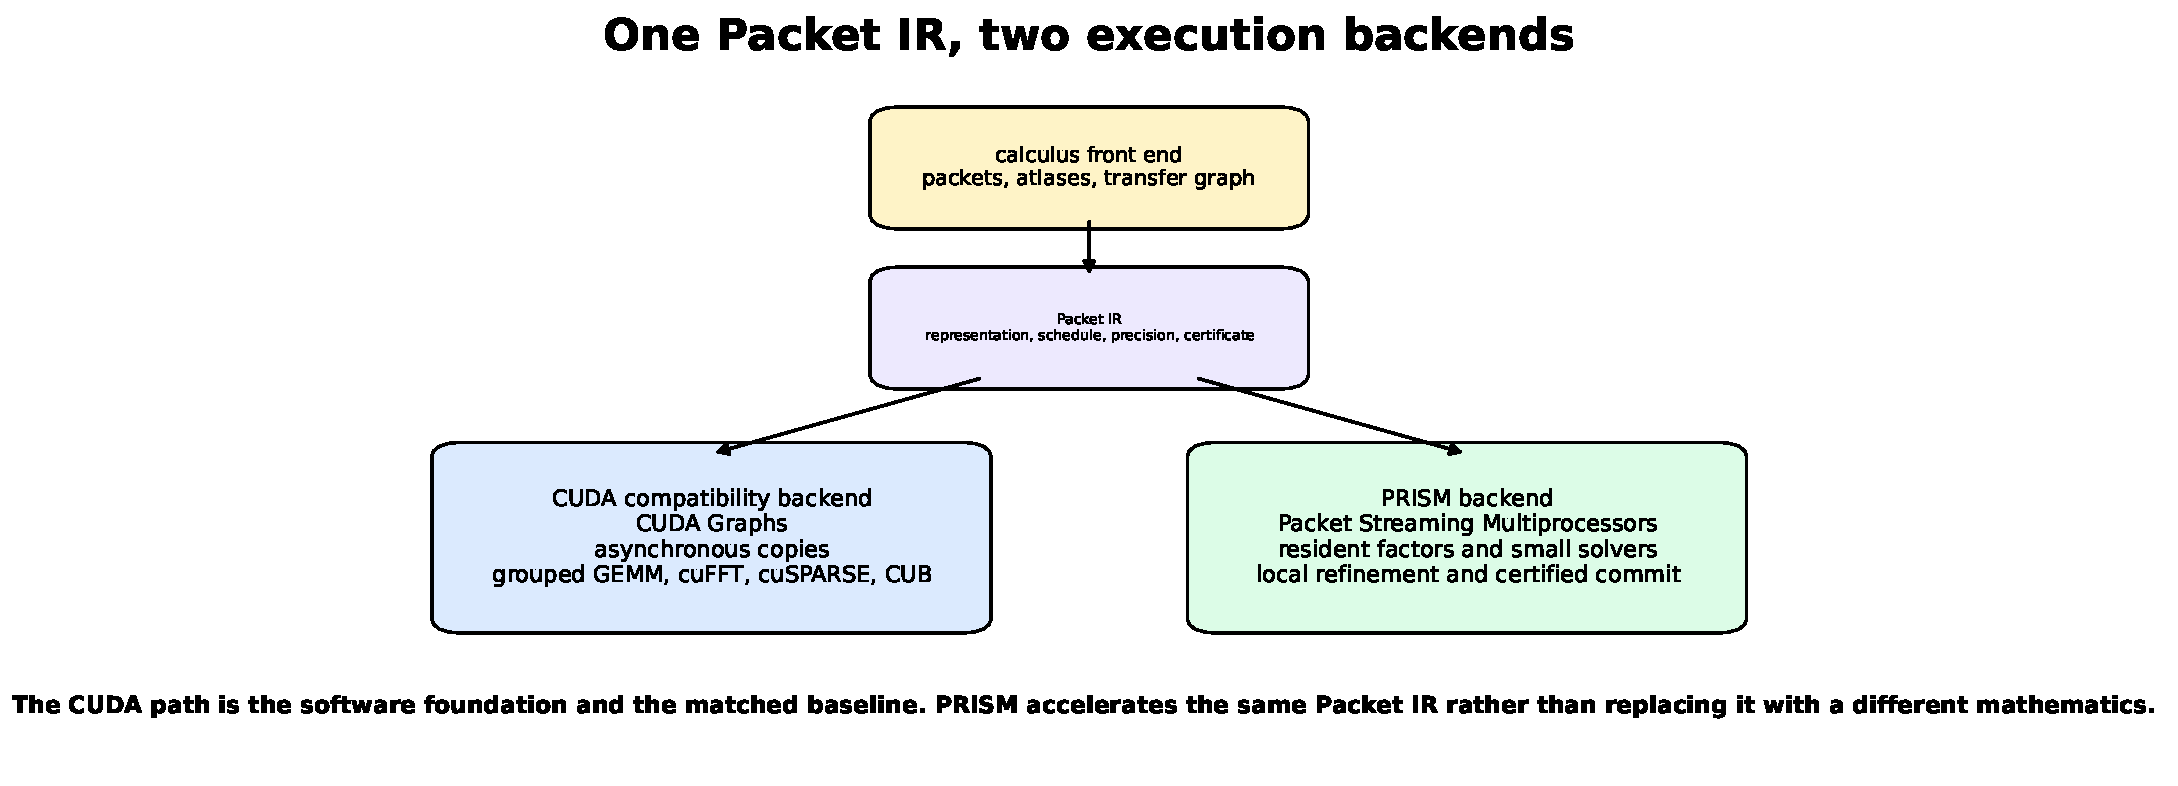
\includegraphics[width=0.94\linewidth]{40_shared_packet_ir.pdf}
\caption{Shared Packet IR makes CUDA the software foundation and matched baseline for PRISM.}
\end{figure}

\section{Compiler flow}
The compiler begins with a typed graph rather than an unstructured kernel list.

\begin{figure}[H]
\centering
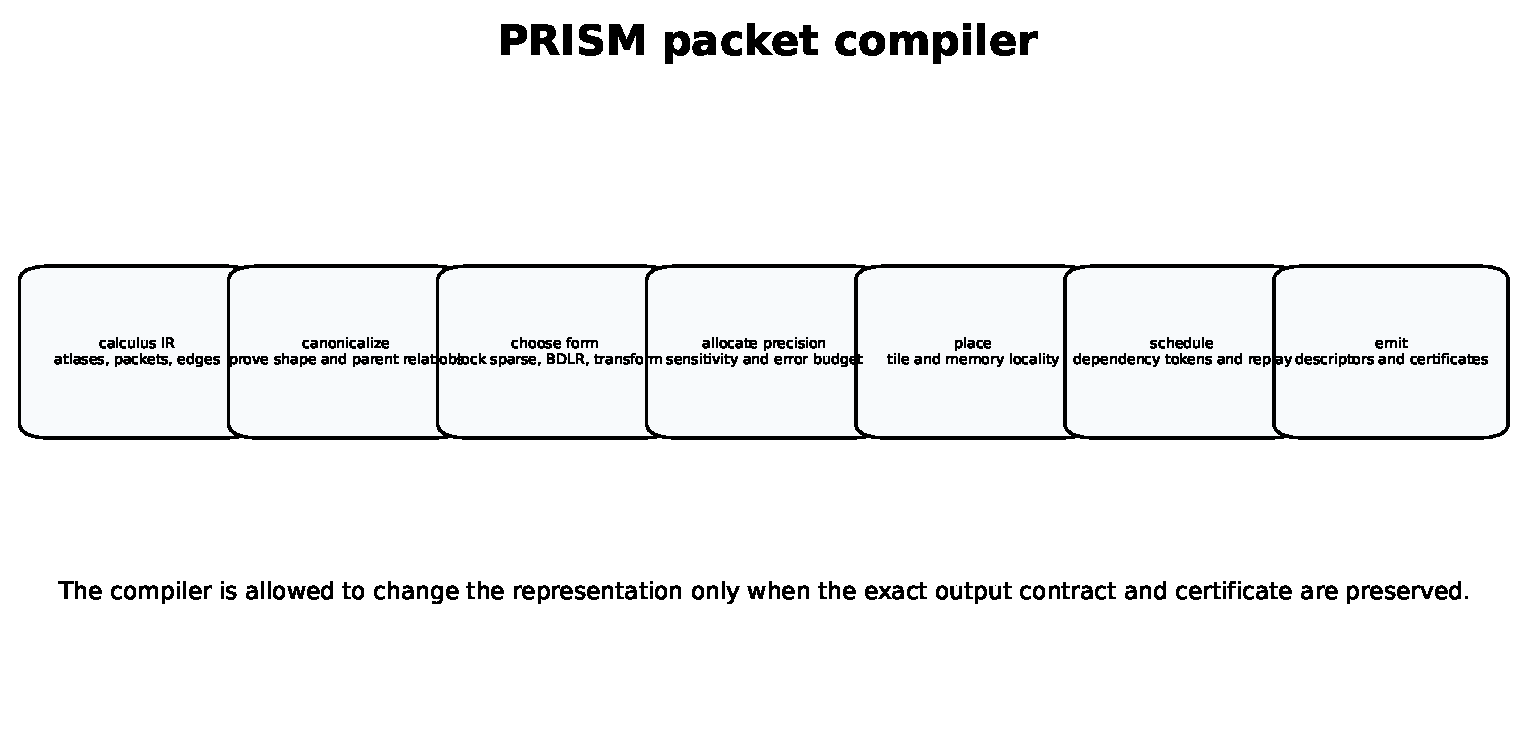
\includegraphics[width=0.98\linewidth]{12_compiler_pipeline.pdf}
\caption{The packet compiler preserves the output contract while changing representation, placement, precision, and schedule.}
\end{figure}

\section{Legality pass}
Before optimization, the compiler checks packet completeness, shape compatibility, parent-child identities, analysis-synthesis pairing, output contracts, and certificate requirements.

\section{Representation pass}
The operator is classified as explicit dense, block diagonal, block sparse, low rank, BDLR, Kronecker, sparse factor chain, transform generated, packet graph, small solver, or nonlinear packet interaction. A form is chosen only when it reduces the declared cost or is required by the output contract.

\section{PMR--GEMM planning}
The representation pass invokes the Bellman planner on the candidate packet tree. The planner considers generic, block, low-rank, Kronecker, sparse-chain, transform, and split choices. The explicit array contract filters out plans that do not return every entry. Apply, factor, and transform contracts leave compressed plans available.

\begin{figure}[H]
\centering
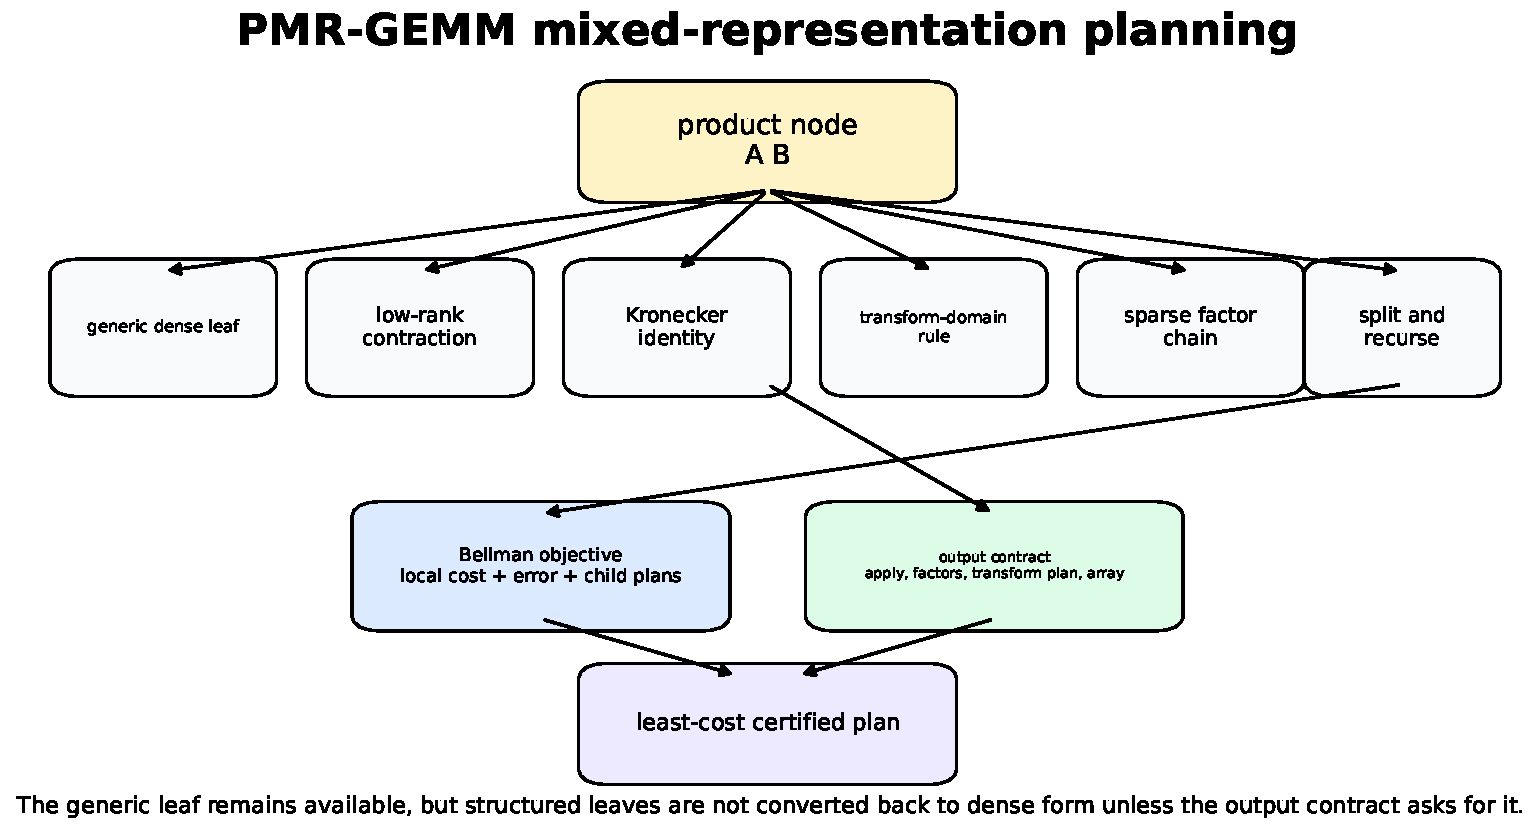
\includegraphics[width=0.95\linewidth]{39_pmr_gemm_planner.pdf}
\caption{The mixed-representation planner selects a certified plan under the requested output contract.}
\end{figure}

\section{Placement and fusion}
The compiler keeps together parent and child packets, diagonal blocks with corresponding factor rows, transform stages sharing one coefficient stream, and small solver chains. Analysis, packet selection, feature reduction, and synthesis may be fused when the exact atlas contract is unchanged.

\section{CUDA compatibility backend}
The CUDA backend maps Packet IR to grouped GEMM, cuBLAS and cuBLASLt, cuFFT, cuSPARSE, CUB reductions, asynchronous copies, stream-ordered allocation, and CUDA Graph replay. It remains the first implementation target and the reference for same-representation comparisons.

\section{PRISM backend}
The PRISM backend replaces launch-heavy graph regions with resident packet warps, PSM scratchpads, representation routing, transform-to-solver handoff, local refinement, and certificate-gated commit. The backend does not change the representation chosen by the compiler unless the cost model requests a new plan.

\section{Worked BDLR compilation}
A BDLR operator enters the compiler as the typed identity $A=D+UV^*$. No explicit matrix is constructed. The legality pass checks dimensions and the requested output form. The representation pass keeps the factors. Placement co-locates each diagonal block with the corresponding rows of $U$ and $V$. Precision is assigned per transfer contribution. The schedule computes $DX$, reduces $V^*X$, broadcasts the small contraction, and forms $U(V^*X)$ locally.

\begin{figure}[H]
\centering
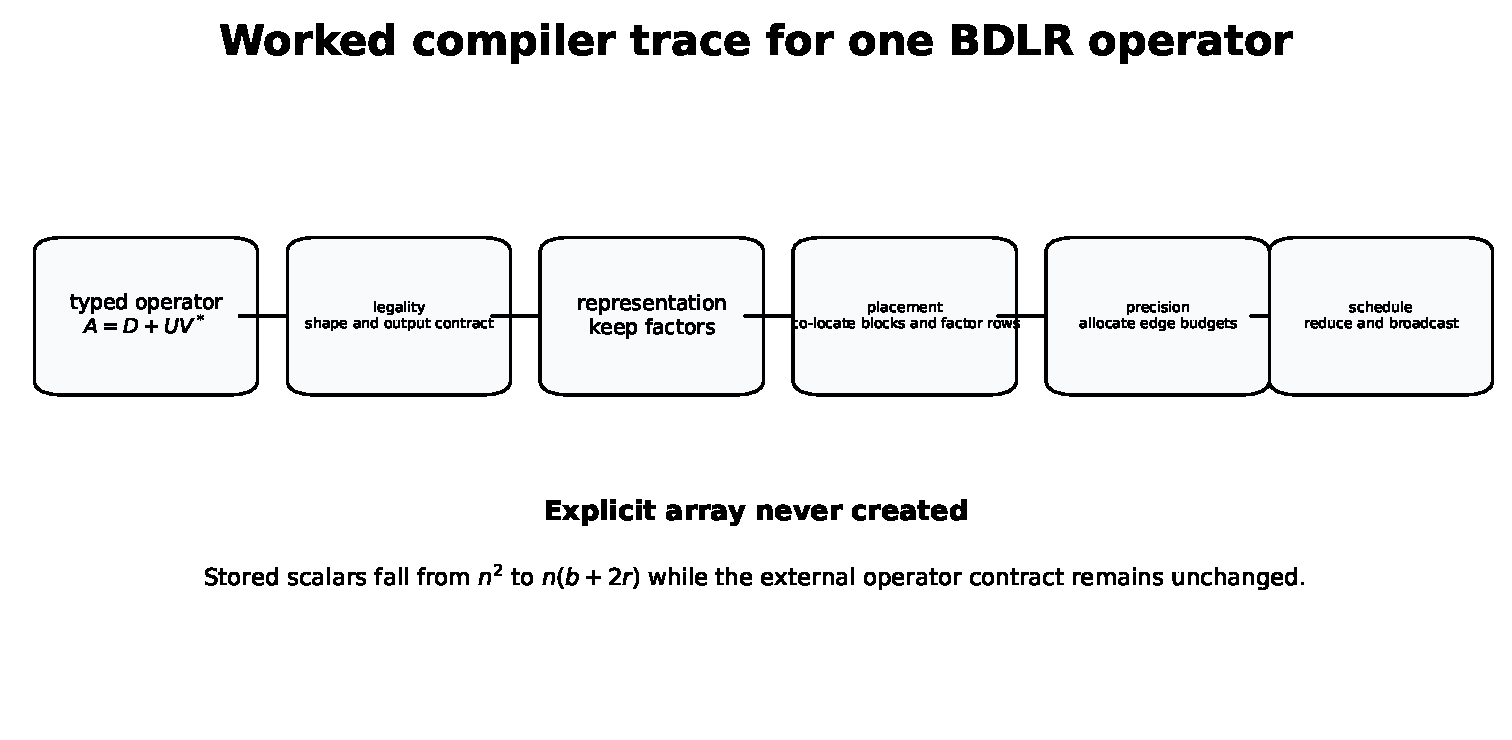
\includegraphics[width=0.96\linewidth]{36_compiler_trace.pdf}
\caption{One BDLR operator through the compiler. The dense matrix is never formed.}
\end{figure}

\section{Certificate plan}
The compiler decides where direct residuals are affordable and where proven upper bounds are used. A graph may contain several certificate boundaries rather than one final check.

\chapter{End-to-end execution traces}

\section{Block diagonal plus low rank}
The host submits packet descriptors for the diagonal blocks and factor rows. The graph contains one block batch, one reduction for $V^*X$, one factor broadcast, one local update, and one certificate. The dense matrix is absent from the graph and from memory.

The external contract is still ordinary matrix application. A direct residual may compare the structured output with a dense reference during bring-up. Production runs can use a proven bound or a spot-check policy when a full dense reference would defeat the representation saving.

\section{Unknown-edge reconstruction}
The transform engine extracts the chosen Fourier packet. The projector DMA groups decimated phase channels. The solver cluster builds the Hankel matrix, estimates rank, finds the annihilator, recovers roots, resolves physical phases, and solves amplitudes. The recovered edge packet is synthesized directly. The smooth residual follows the spectral path. A final residual and branch-margin record are written before commit.

\section{One PR-LASM step}
The exact archive remains in HBM. Macro, meso, and micro states remain in SRAM. Mechanism families reuse the same state matrices. The small solvers update their posterior records. The planner reads exact transition edges separately from probabilistic predictions. A large residual can request local packet refinement without invalidating the rest of the graph.

\section{Why these traces matter}
The three examples use different engines but share one architectural pattern. The representation remains typed, local work is scheduled by dependency tokens, intermediate factors remain resident, and the result is not committed until the declared check passes.

\chapter{Compositional correctness}

\begin{theorem}[Hardware reconstruction theorem]
Let a finite calculus graph have exact packet analysis and synthesis, exact transfer kernels, and an acyclic dependency graph. Suppose every hardware command implements its declared local map and every packet sum uses the declared complete family. Then the committed hardware output equals the mathematical graph output.
\end{theorem}

\begin{proof}
Order the graph topologically. Each source command loads the declared seed or packet. Assume every predecessor of a node has the correct value. The command implements the node's declared local map, so the node output is correct. Packet accumulation is exact because the declared child or source family is complete. Induction reaches every sink. The final synthesis therefore equals the mathematical graph output. The commit command changes status, not value.
\end{proof}

\begin{theorem}[Certified commit]
Suppose a command result is provisional until a certificate $c(y)$ is evaluated. If the commit controller releases $y$ only when $c(y)$ satisfies the declared acceptance rule, then every visible result has passed that rule. A failed result cannot satisfy a downstream completion token.
\end{theorem}

\begin{proof}
The provisional buffer is not addressable through the committed packet directory. Passing the rule changes the directory state and releases the completion token. Failure leaves the committed state unchanged and redirects the declared graph region to replay or abort. Downstream commands therefore cannot observe an unchecked value through the normal dependency path.
\end{proof}

\begin{corollary}[Local refinement correctness]
If a parent packet is replaced by a child graph whose synthesis equals the parent interface, the refined hardware graph has the same external mathematical output.
\end{corollary}

\begin{proof}
The topological-splice theorem gives a legal schedule. Exact child synthesis gives the same value at the parent interface. Every downstream command therefore receives the same input.
\end{proof}

\chapter{Performance accounting}

\section{Four different sources of gain}
A fair result must say what changed. The total route may improve because the mathematics removed work, because the same representation ran better on another device, because a kernel was fused or graph-replayed, or because one-time setup was amortized. These are different quantities:
\[
S_{\mathrm{total}}
=
S_{\mathrm{representation}}
S_{\mathrm{architecture}}
S_{\mathrm{kernel}}
S_{\mathrm{amortization}}.
\]
This is a bookkeeping identity only when every factor comes from matched rows with the same output contract and timing scope. Otherwise the factors are reported separately.

\begin{figure}[H]
\centering
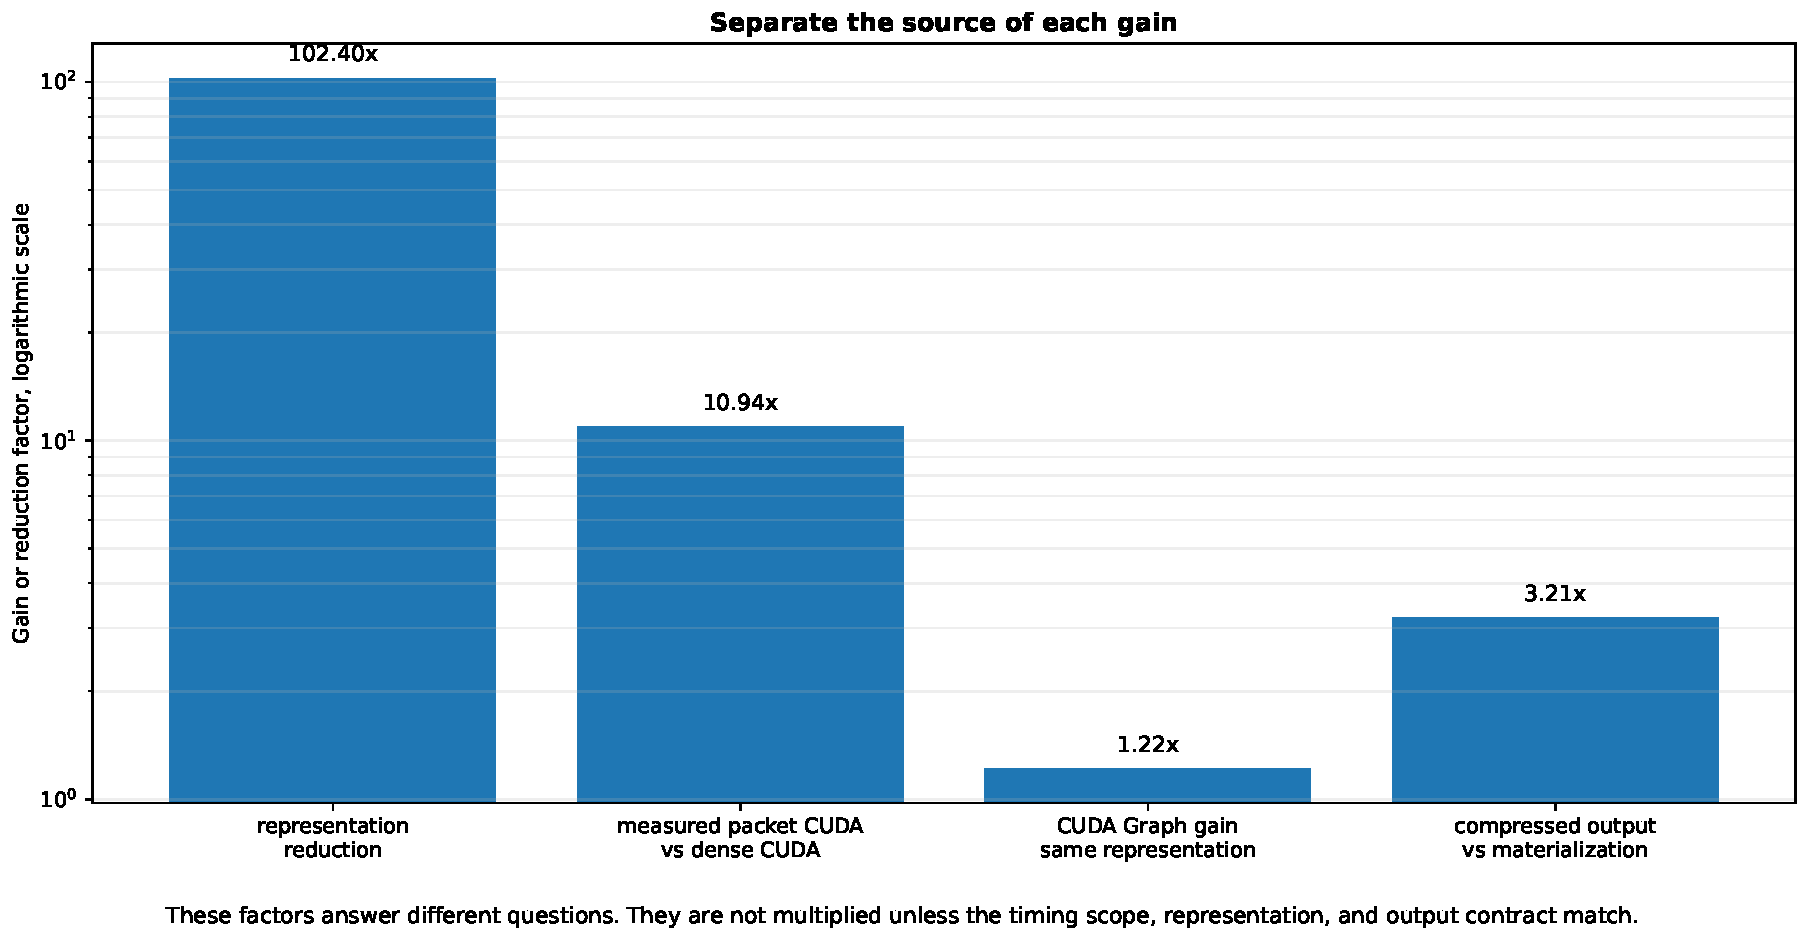
\includegraphics[width=0.92\linewidth]{41_gain_decomposition.pdf}
\caption{Representation, packet-CUDA, graph-replay, and output-contract gains answer different questions.}
\end{figure}

\section{Measured CUDA foundation}
The prior packet-GPU study contains 154 matched CPU and GPU rows. The recorded GPU is an RTX 3070 Ti Laptop GPU. For $n=8192$, block width $64$, and 32 right-hand sides, the equal-block packet path took $0.046032$ ms and was $14.8919\times$ faster than the matched device-resident dense GPU row. For BDLR with rank eight, the standard packet path took $0.097280$ ms and CUDA Graph replay took $0.079872$ ms. The graph row was $10.9355\times$ faster than the matched dense GPU row. The graph improvement over the standard packet path was about $1.218\times$.

A compressed BDLR product at $n=1024$ took $0.1582$ ms. Materializing the explicit output took $0.5073$ ms. Those rows have different output contracts. The comparison shows the cost of requesting every entry. It is not a claim that one result is a faster implementation of the other.

\begin{figure}[H]
\centering
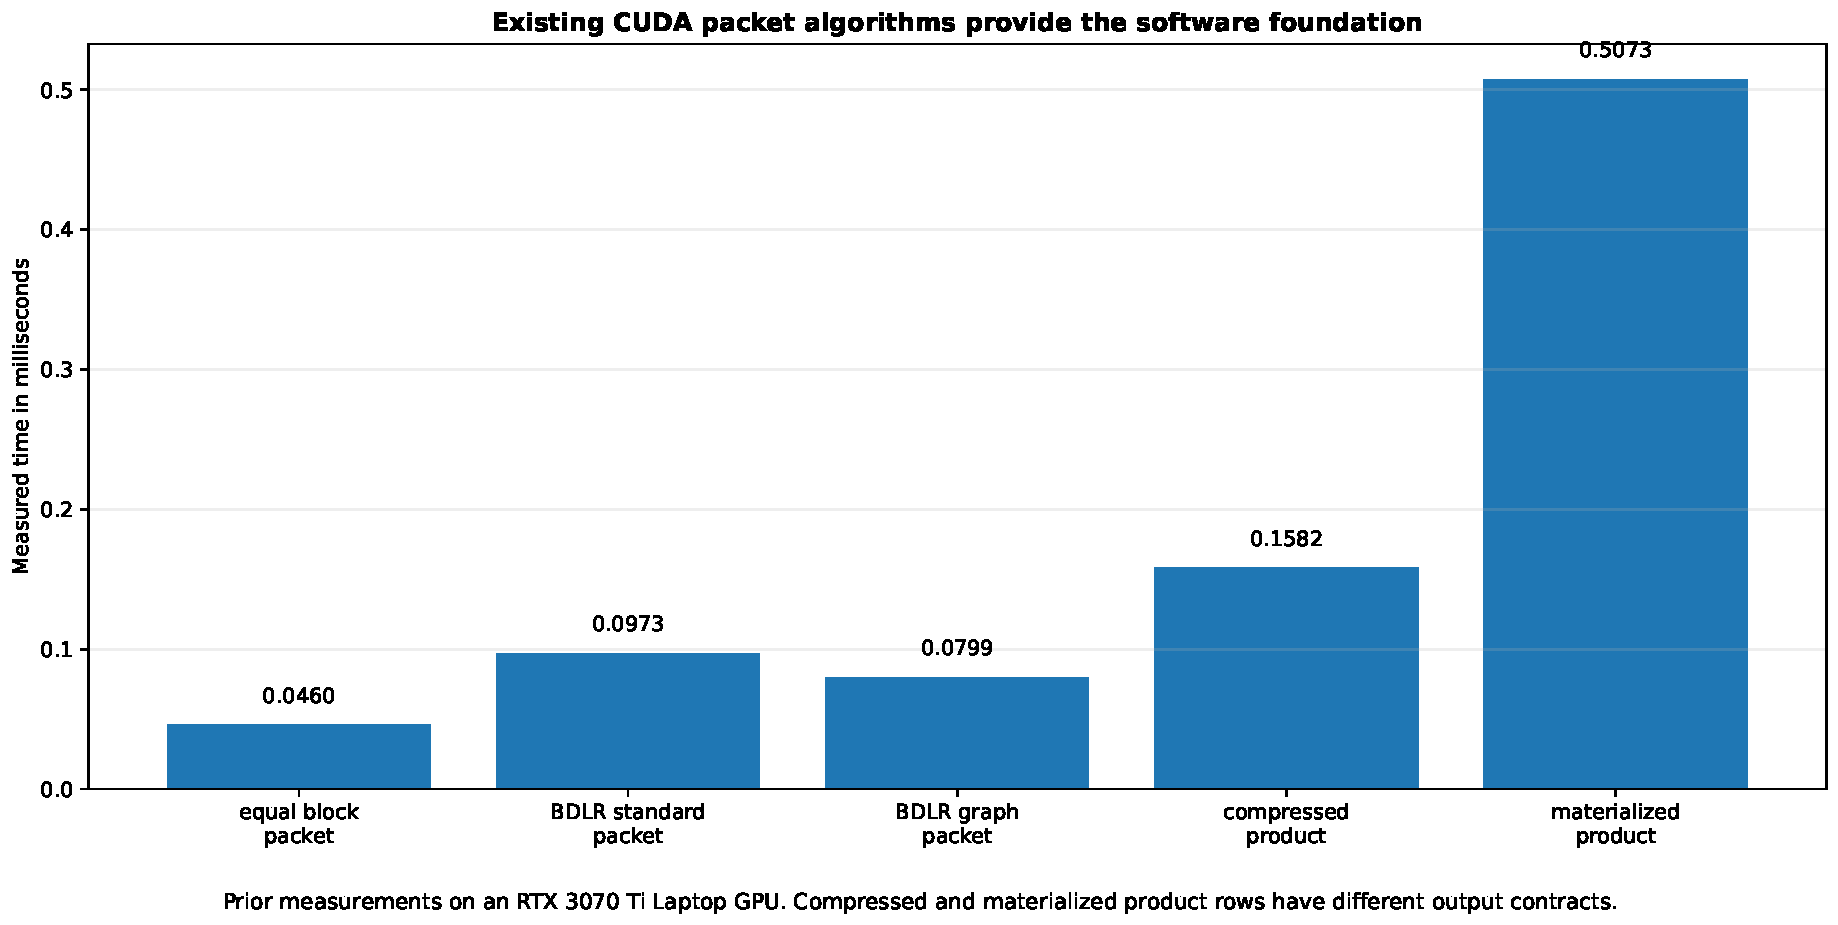
\includegraphics[width=0.91\linewidth]{43_cuda_measured_baselines.pdf}
\caption{Measured CUDA packet timings from the earlier structured-operator study.}
\end{figure}

\section{Representation reduction}
For
\[
A=D+UV^*,
\]
with dimension $n$, block width $b$, rank $r$, and $q$ right-hand sides, a factor-first application uses
\[
2qn(b+2r)
\]
modeled operations and stores
\[
n(b+2r)
\]
scalars. The corresponding dense counts are $2qn^2$ and $n^2$. For
\[
n=8192,
\qquad b=64,
\qquad r=8,
\qquad q=32,
\]
the arithmetic and storage reduction is
\[
\boxed{\frac{n}{b+2r}=102.4.}
\]
This reduction belongs to the representation. A CUDA backend and a PRISM backend can both use it.

\section{PRISM architecture model}
The architecture model uses
\[
T=
\max\left(
\frac{F}{\eta_cP},
\frac{B}{\eta_bW}
\right)
+T_{\mathrm{graph}},
\]
where $F$ is arithmetic, $B$ is data movement, $P$ is peak arithmetic, $W$ is bandwidth, and $\eta_c$, $\eta_b$ are efficiency factors. The model is used to decide which hardware paths are worth building. It is not a silicon measurement.

\begin{figure}[H]
\centering
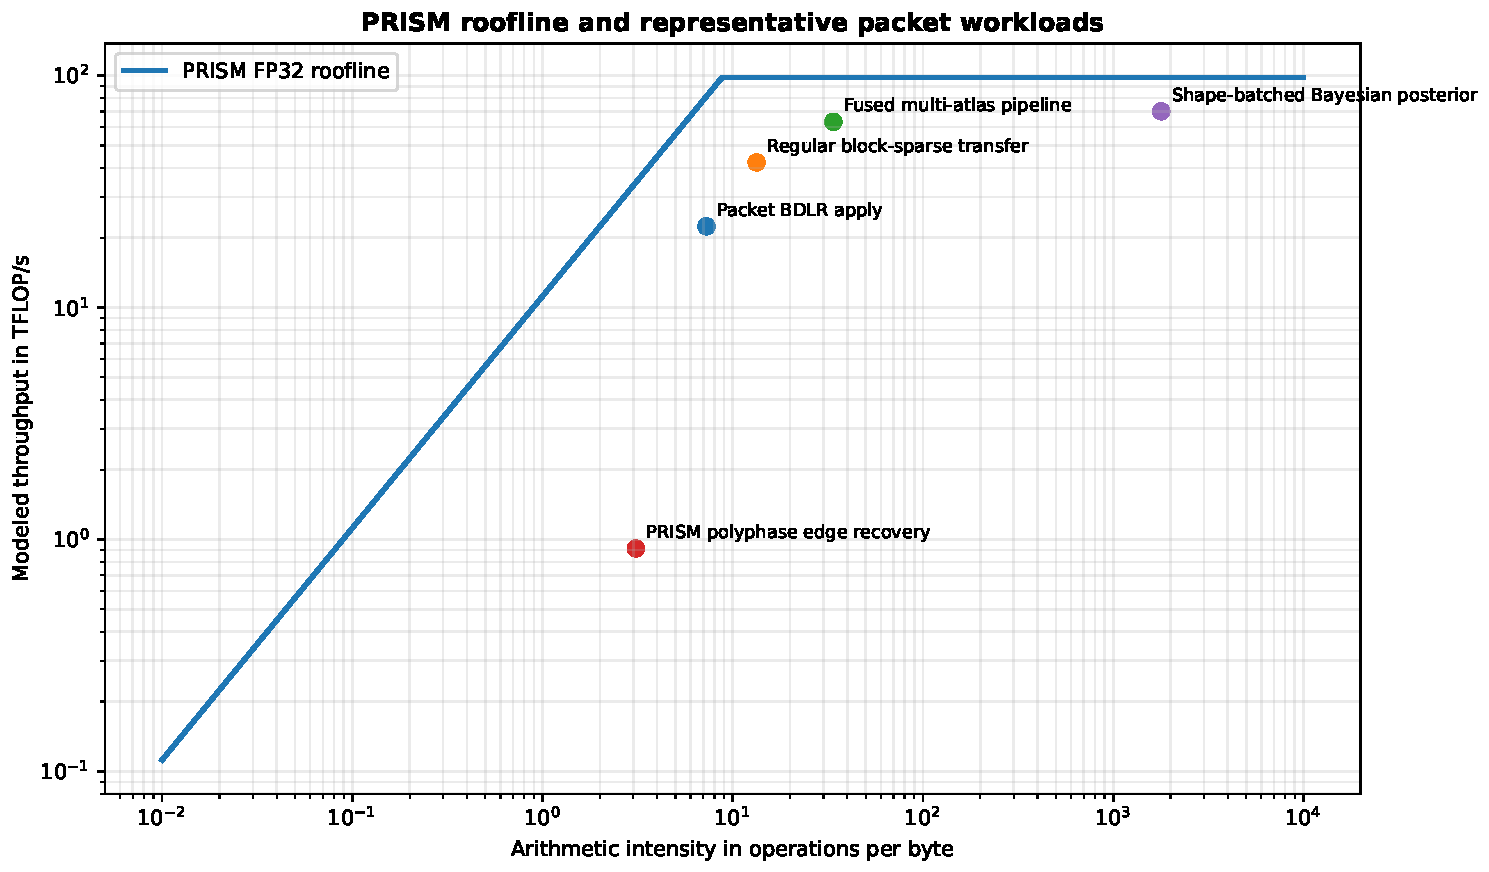
\includegraphics[width=0.84\linewidth]{14_roofline.pdf}
\caption{Reference PRISM roofline with representative packet workloads.}
\end{figure}

\section{Total route model and architecture-only models}
The earlier dense-route comparison predicts $70.79$ microseconds for a dense application and $1.87$ microseconds for the PRISM BDLR route. The ratio is about $37.8$. This is a total route model. It includes representation reduction and therefore is not labeled PRISM-over-CUDA architecture gain.

The more relevant architecture models begin with the same structured pipeline on both sides. They estimate:
\begin{center}
\begin{tabular}{lrr}
\toprule
Workload & Generic structured path & PRISM path \\
\midrule
Fused multi-atlas analysis & $14.73$ $\mu$s & $8.96$ $\mu$s \\
Polyphase edge recovery & $4.00$ $\mu$s & $1.35$ $\mu$s \\
Bayesian model portfolio & $427.93$ $\mu$s & $300.52$ $\mu$s \\
\bottomrule
\end{tabular}
\end{center}
The corresponding modeled gains are $1.64\times$, $2.96\times$, and $1.42\times$. These are the present estimates of what residency, fusion, local solvers, and packet scheduling may add after a structured representation is already in use.

\section{Sensitivity and crossover}
No single row should define the architecture. BDLR gains depend on block width and correction rank. Transform gains depend on size, reuse, and fusion. Sparse graphs depend on regularity. Small solvers depend on batch size and handoff cost.

\begin{figure}[H]
\centering
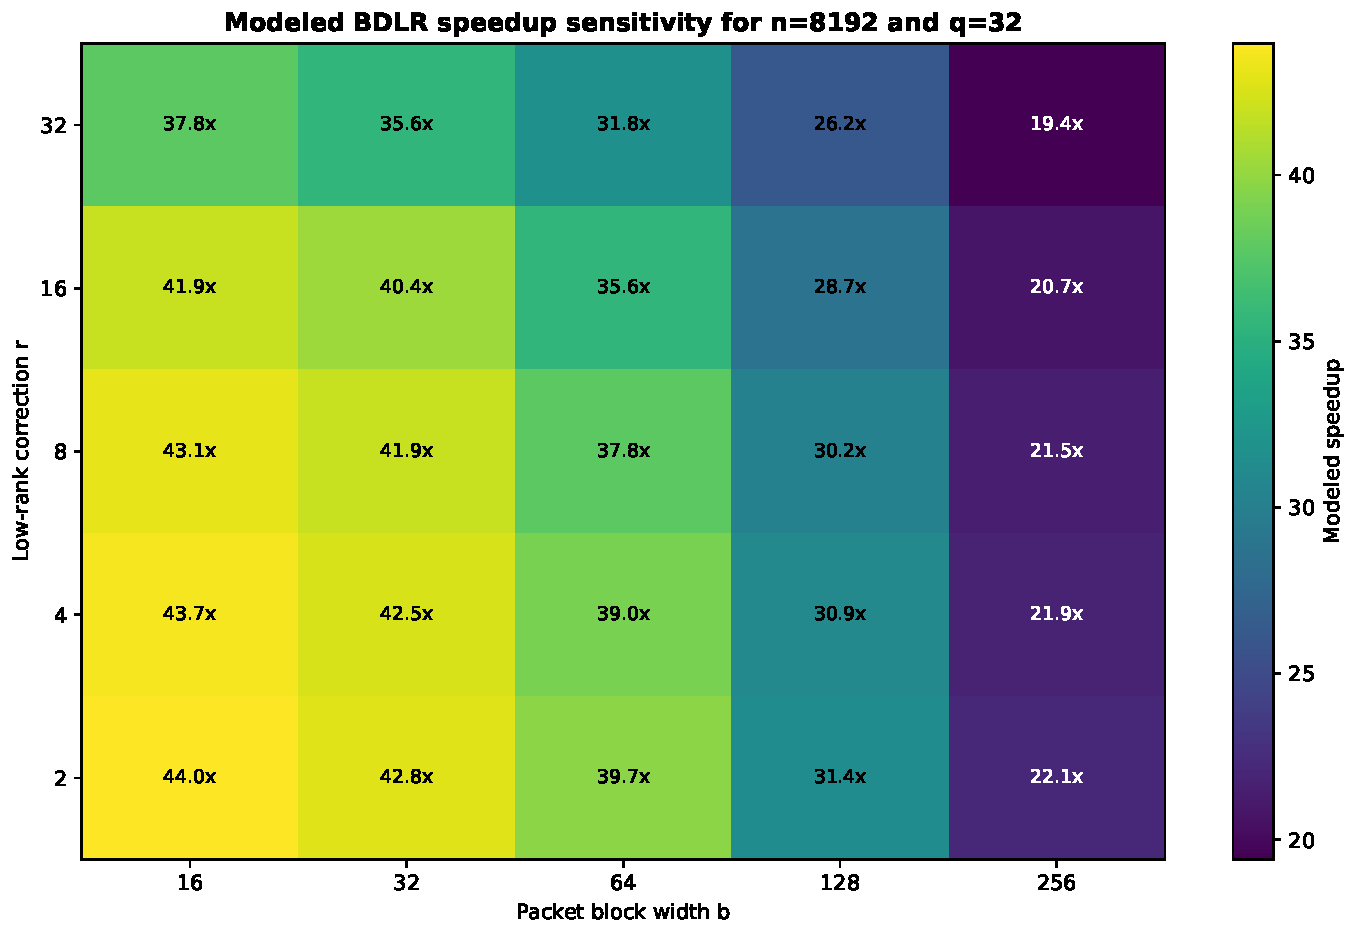
\includegraphics[width=0.84\linewidth]{29_bdlr_speedup_sensitivity.pdf}
\caption{Total route sensitivity across block width and correction rank.}
\end{figure}

\begin{figure}[H]
\centering
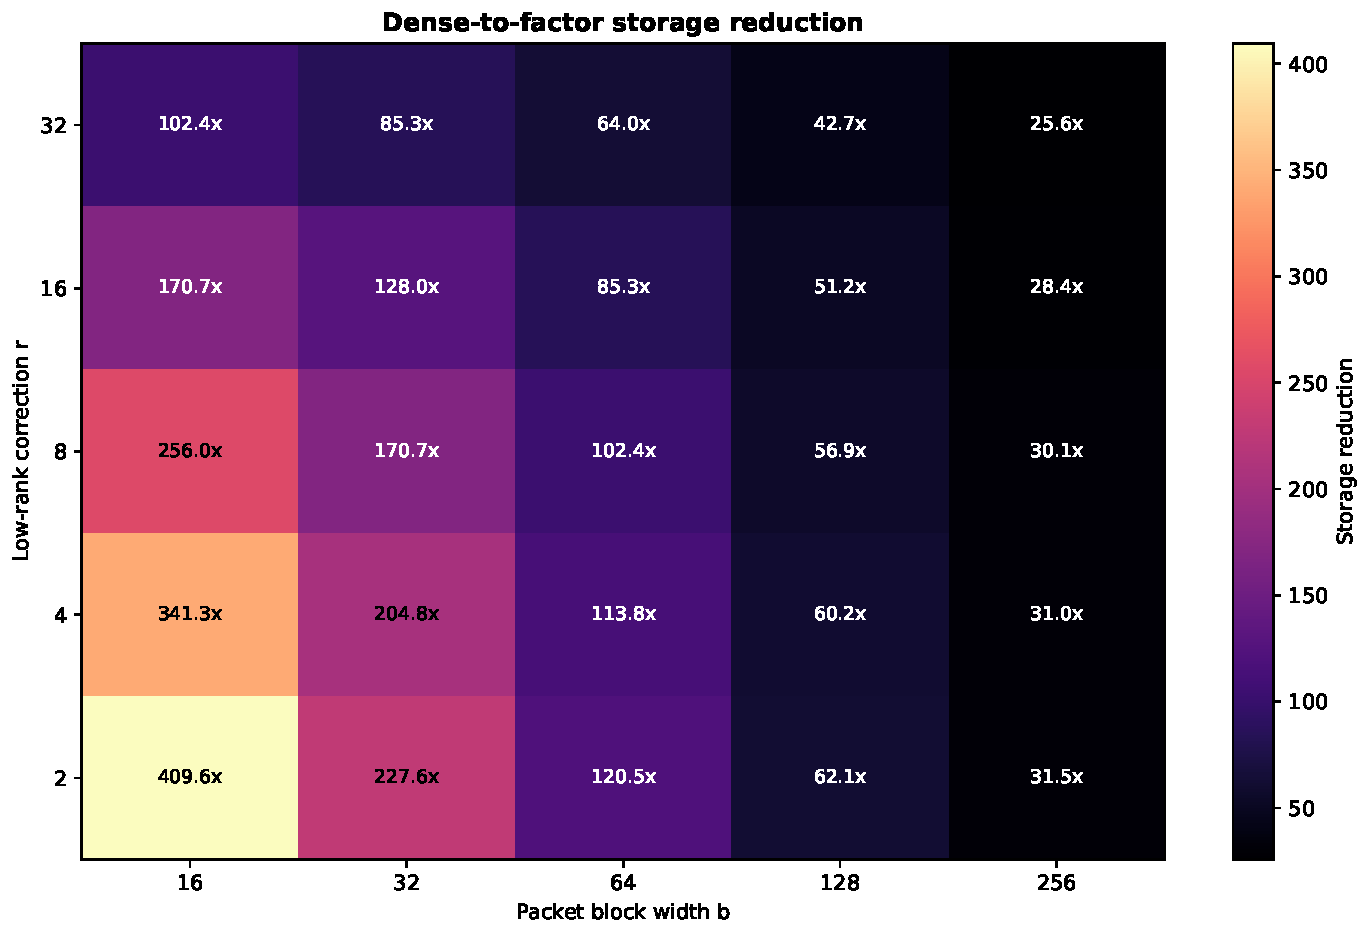
\includegraphics[width=0.84\linewidth]{30_bdlr_storage_sensitivity.pdf}
\caption{Representation-storage reduction across block width and correction rank.}
\end{figure}

\section{Negative controls}
The earlier CUDA study retained cases where structure lost. Recursive HODLR was slower than dense GPU execution in the tested case. A GPU Walsh-Hadamard transform lost to the CPU at the smaller tested length. A two-stream dense pipeline lost to the serial path. Iterative refinement lost to a direct FP64 solve. The PRISM compiler must preserve these negative controls and route similar work away from specialized paths.

\begin{figure}[H]
\centering
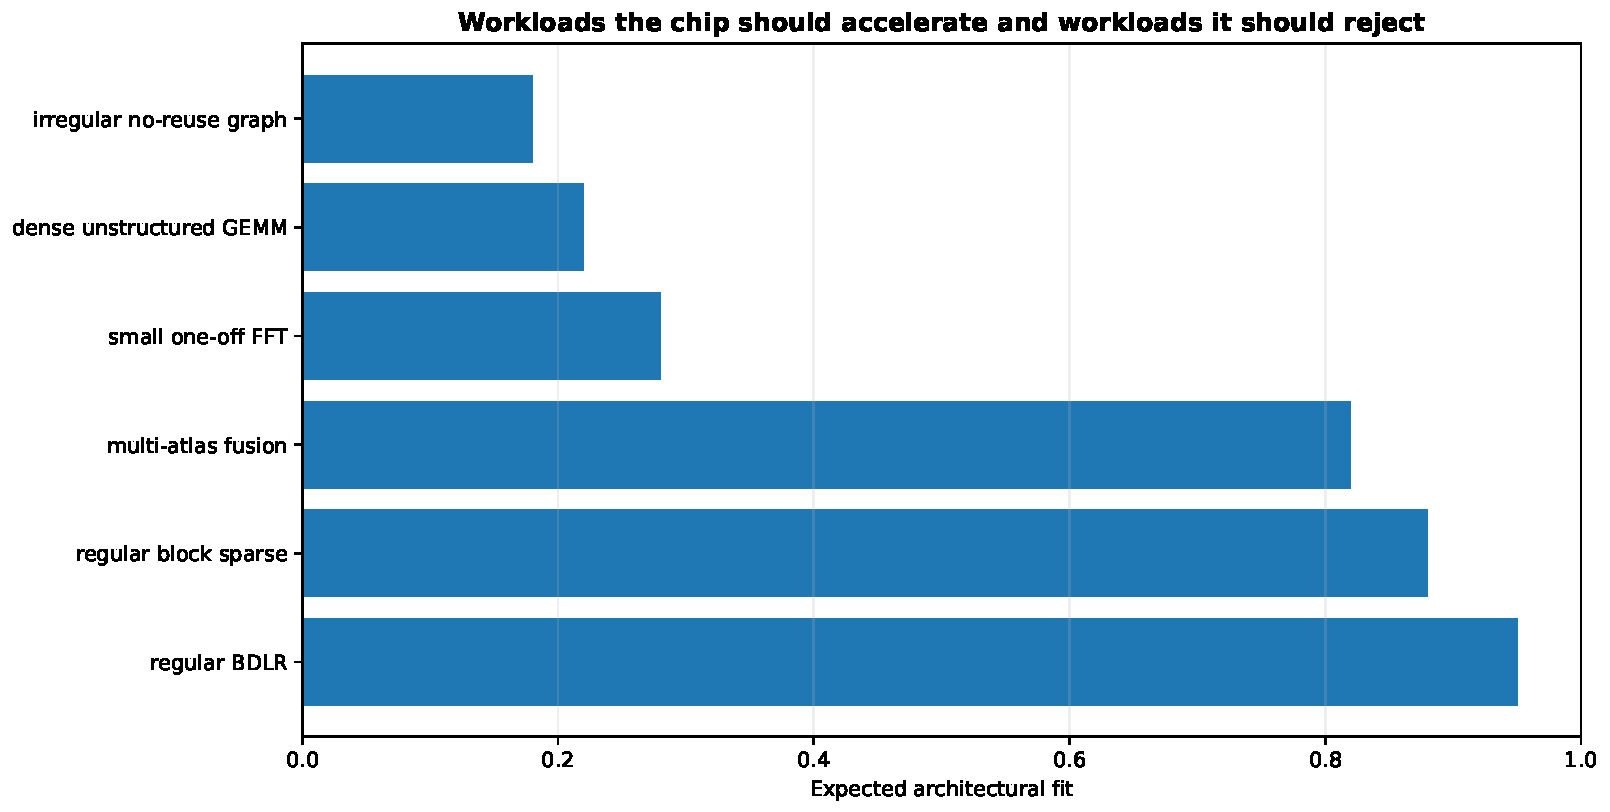
\includegraphics[width=0.86\linewidth]{23_workload_fit.pdf}
\caption{PRISM should accelerate strong reusable structure and reject weak or one-off structure.}
\end{figure}

\chapter{Power, area, and thermal design}

\section{Power budget}
The reference package targets a 500 W envelope. The model allocates power to execution groups, SRAM, the packet network, HBM PHYs, transform and solver blocks, control, and margin.

\begin{figure}[H]
\centering
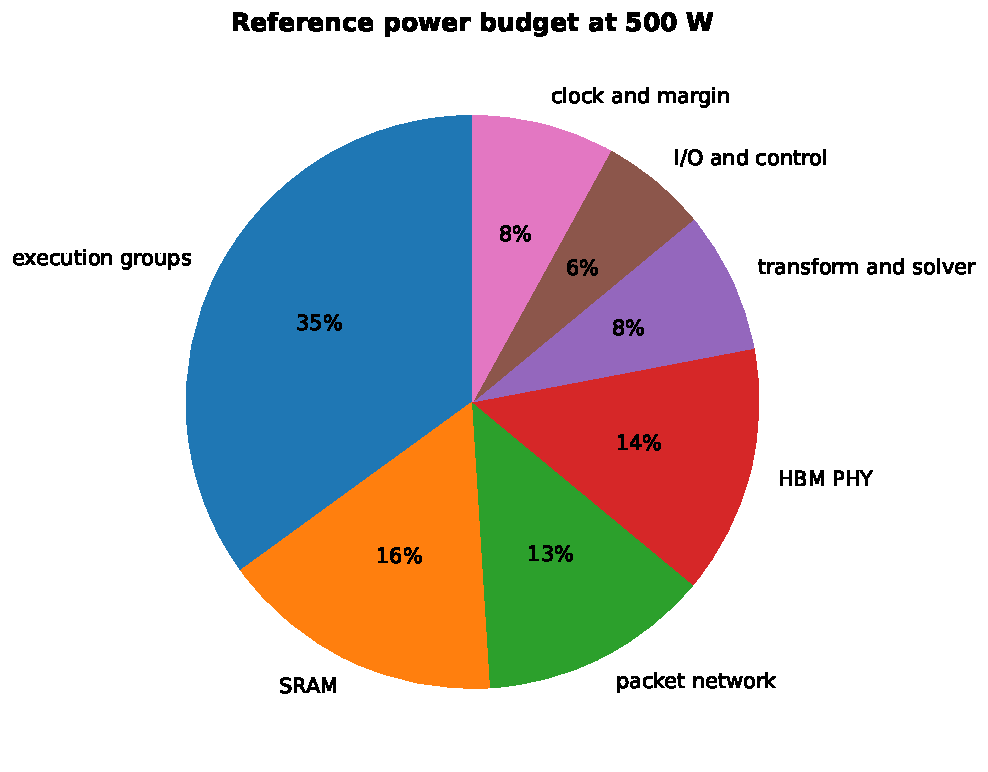
\includegraphics[width=0.72\linewidth]{17_power_budget.pdf}
\caption{Reference power allocation.}
\end{figure}

\section{Area allocation}
Distributed SRAM is the largest target area because the architecture depends on resident packets and factors. Matrix and vector lanes occupy the next largest share.

\begin{figure}[H]
\centering
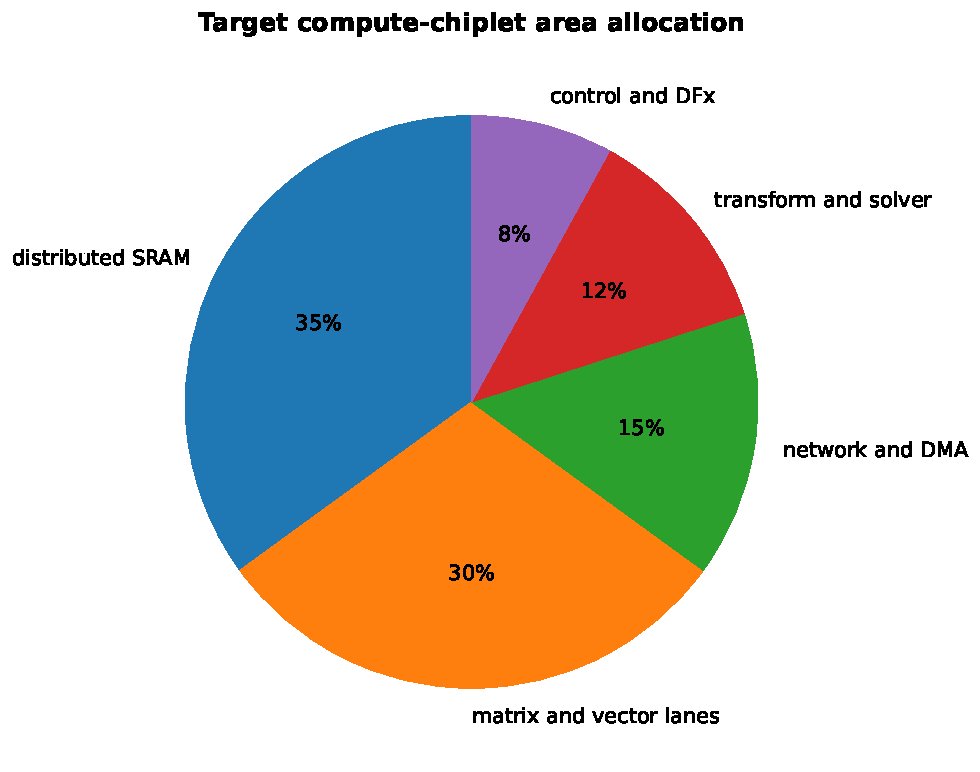
\includegraphics[width=0.72\linewidth]{18_area_allocation.pdf}
\caption{Target compute-chiplet area allocation.}
\end{figure}

\section{Thermal behavior}
The scheduler can spread long transform and matrix batches across chiplets. UCIe priority sideband and fast-throttle features are natural matches for package-wide thermal events. Local descriptor replay can be paused without discarding the packet graph.

\chapter{Reliability, protection, and recovery}

\section{Protected state}
Packet descriptors, transfer descriptors, dependency tokens, and certificate records control meaning as well as data movement. They require stronger protection than ordinary cache metadata. The reference plan uses ECC for SRAM-resident tables, parity on command queues, sequence numbers on replay regions, and end-to-end tags on HBM packet records.

\section{Failure containment}
An execution-group or PSM error should not force a package-wide reset unless the packet directory or global scheduler has lost coherence. Local kernel faults invalidate the destination packet and its descendants. A link or memory fault invalidates every packet whose provenance crosses the failed resource. The compiler emits provenance information so the runtime can identify the affected region.

\section{Determinism}
Deterministic mode fixes the reduction tree, solver ordering, and replay schedule. It is slower than the highest-throughput mode. Its purpose is bring-up, regression testing, exact replay, and certificate comparison.

\section{Security boundary}
The architecture does not introduce a new trust model. Host isolation, command validation, memory protection, firmware signing, and secure update remain required. Packet descriptors make the dataflow easier to audit, but they do not replace platform security.

\chapter{Programming model}

\section{Four software layers}
The software stack has four levels:
\begin{enumerate}
\item a high-level calculus graph
\item shared Packet IR
\item CUDA or PRISM backend lowering
\item Packet Seed Commands, descriptor tables, and the runtime queue
\end{enumerate}
The release includes JSON examples for BDLR application, PMR--GEMM planning, self-calibrating edge recovery, and a PR-LASM step.

\section{Host control}
RISC-V management cores run the command runtime, graph loader, memory manager, telemetry, and error handling. The CUDA backend uses the same Packet IR before final lowering. Ordinary vector code handles control-side data preparation. The accelerator command queue is the stable interface to the packet engines.

\section{Device libraries}
A practical library should expose:
\begin{itemize}
\item packet and atlas construction
\item transform analysis and synthesis
\item transfer graph creation
\item BDLR and block-sparse operators
\item edge-recovery graphs
\item Bayesian program batches
\item certificate policies
\item graph replay and local refinement
\end{itemize}

\chapter{Verification}

\section{Verification ladder}
The architecture is specified so each development stage has a clear target. Mathematical contracts come first. The behavioral model checks those contracts. Bit-accurate kernels then define rounding and exception behavior. RTL simulation and formal properties check control. An FPGA overlay measures real data movement before a chiplet is attempted.

\begin{figure}[H]
\centering
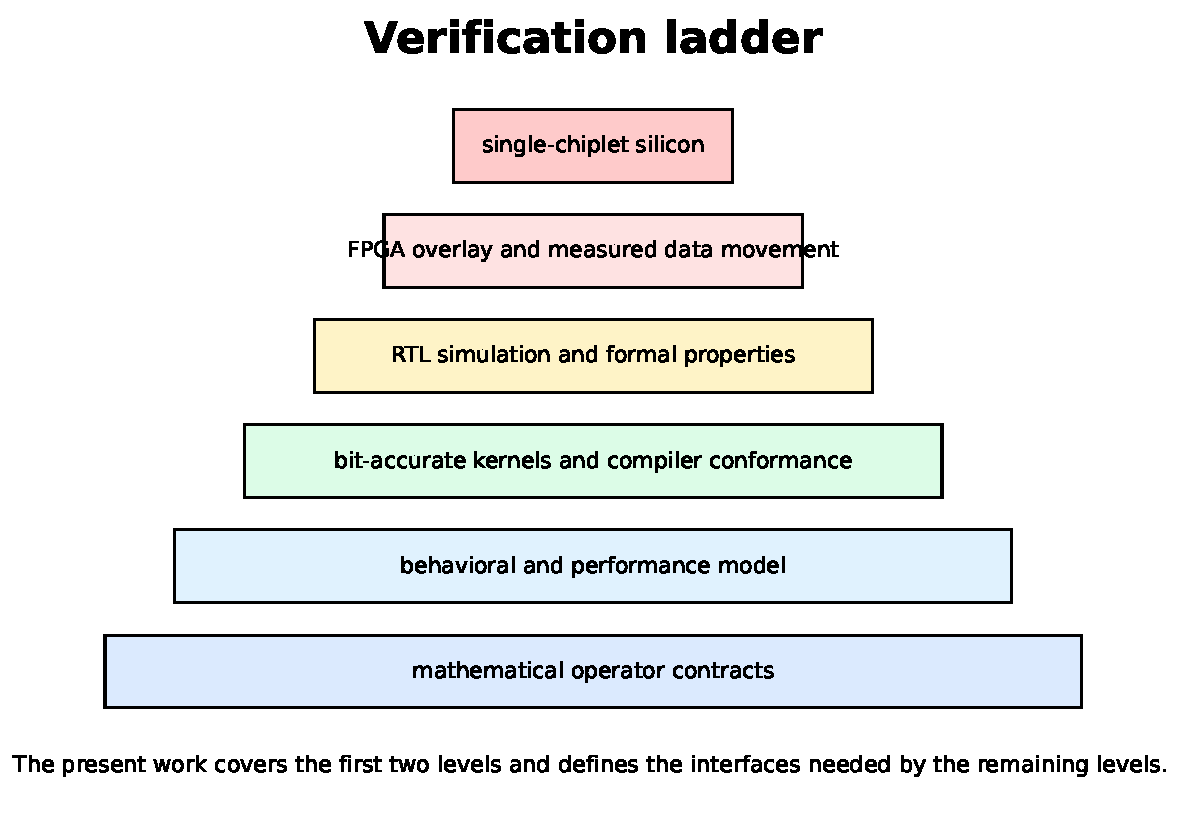
\includegraphics[width=0.74\linewidth]{33_verification_pyramid.pdf}
\caption{Verification ladder from mathematical contracts to measured silicon.}
\end{figure}

\section{Behavioral tests}
The executable model currently verifies:
\begin{itemize}
\item complete residue-packet reconstruction
\item exact polyphase round trip
\item exact Haar round trip
\item BDLR factor execution against dense materialization
\item local DAG substitution
\item derived package totals
\item descriptor contracts
\item precision-budget allocation
\item certificate-gated commit
\item local refinement descriptor bounds
\item compiler routing decisions
\item BDLR sensitivity tables
\item package bandwidth hierarchy
\item Packet Streaming Multiprocessor hierarchy
\item PMR--GEMM Bellman planning
\item output-contract legality without mandatory dense state
\item measured CUDA baseline registry
\item typed gain decomposition
\end{itemize}

\begin{certificate}[Current executable result]
The behavioral and architecture model passes
\[
\boxed{18/18\text{ self-tests}}
\]
and the independent pytest suite passes
\[
\boxed{18/18\text{ tests}.}
\]
The largest semantic residual is the BDLR comparison residual
\[
1.42\times10^{-14},
\]
which is consistent with floating-point roundoff.
\end{certificate}

\section{RTL boundary}
The release contains a SystemVerilog architecture skeleton for descriptors, command buffering, dependency tokens, the packet directory, representation routing, PSM scheduling, execution-group control, the residual path, certificate-gated commit, and the top-level queue interface. No HDL compiler or synthesis tool was available in the build environment. The RTL skeleton is therefore not described as verified or synthesizable silicon.

\section{What must be verified before tapeout}
A serious implementation requires:
\begin{itemize}
\item bit-accurate kernel models
\item formal checks of command ordering and descriptor protection
\item CDC and reset verification
\item UCIe, HBM, PCIe, and optional CXL compliance IP integration
\item SRAM and NoC timing closure
\item thermal and power-integrity analysis
\item fault injection for replay and certificate failure
\item compiler and runtime conformance suites
\end{itemize}

\chapter{Implementation path}

\begin{figure}[H]
\centering
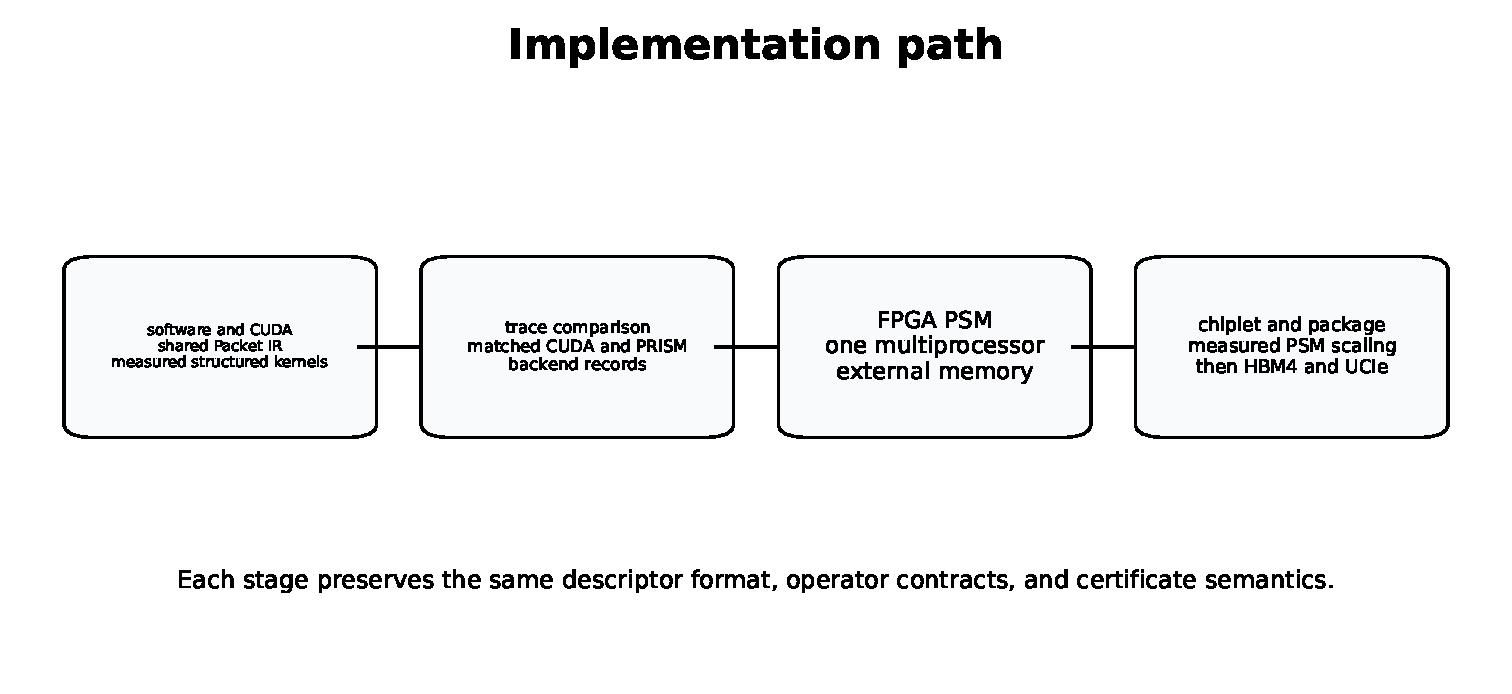
\includegraphics[width=0.95\linewidth]{22_implementation_path.pdf}
\caption{The software and CUDA stages precede FPGA and silicon work.}
\end{figure}

\section{Stage 1: software and CUDA foundation}
The calculus already has CPU references, CUDA packet kernels, grouped block execution, compressed BDLR products, Woodbury solves, CUDA Graph replay, mixed-precision certificates, transform paths, and measured structured-operator baselines. This stage supplies the semantics, Packet IR, workload traces, and matched comparison.

\section{Stage 2: trace-driven backend comparison}
The next software stage lowers the same Packet IR to CUDA and to the PRISM simulator. It records representation, bytes, arithmetic, launch count, solver size, reuse, residual, and output contract. This stage identifies the graph regions that remain bottlenecked after CUDA has already used the better algorithms.

\section{Stage 3: FPGA Packet Streaming Multiprocessor}
The FPGA overlay should implement one Packet Streaming Multiprocessor, packet DMA, one transform path, one matrix and factor path, one small solver, the packet directory, dependency tokens, residual accumulation, and certificate-gated commit. The descriptor and Packet IR formats should match the later ASIC.

\begin{figure}[H]
\centering
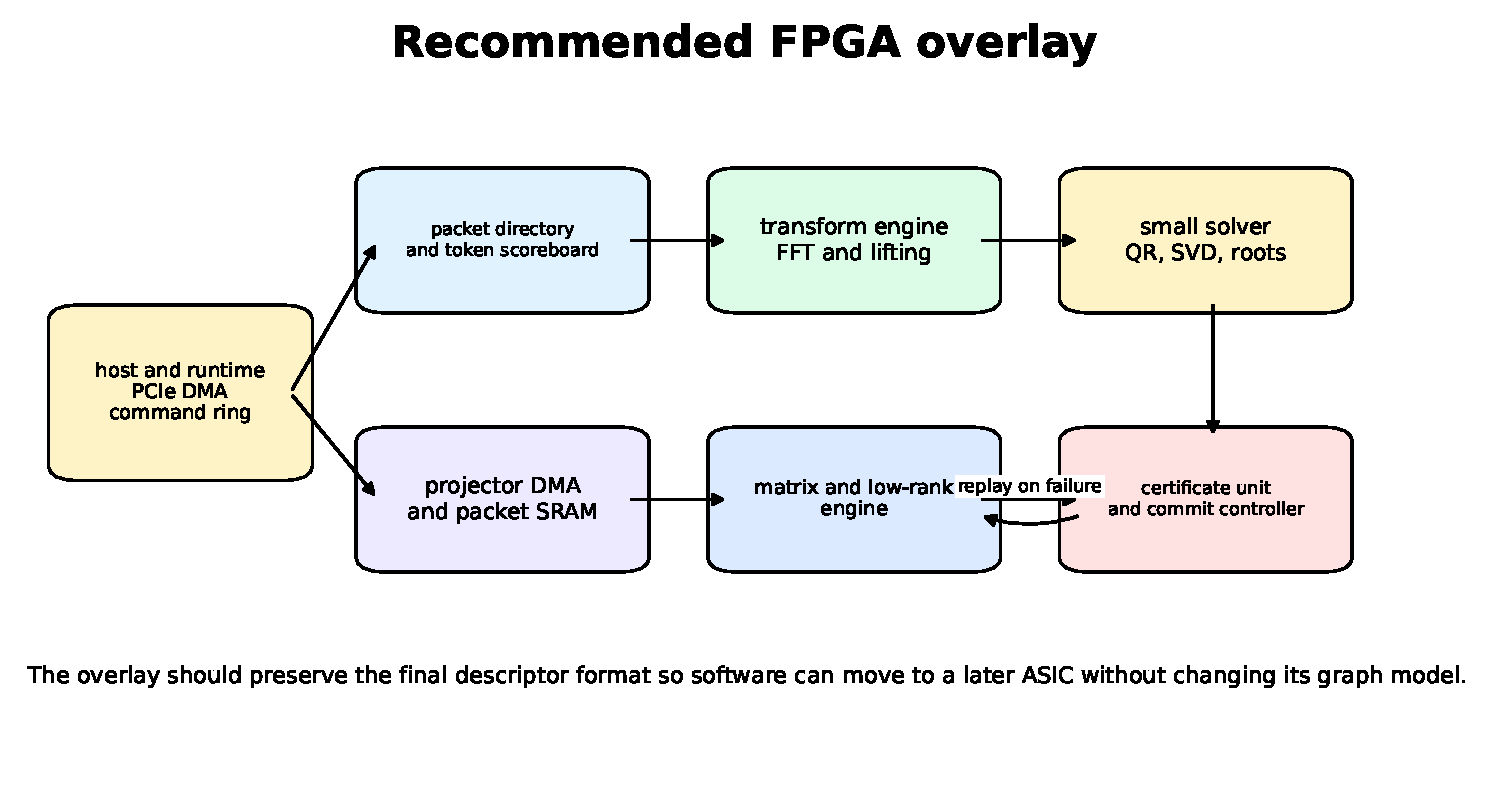
\includegraphics[width=0.95\linewidth]{34_fpga_overlay.pdf}
\caption{Recommended FPGA overlay for measuring the architectural features that do not reduce to an ordinary CUDA kernel.}
\end{figure}

\section{Stage 4: one compute chiplet}
A shuttle-scale device can use four to eight Packet Streaming Multiprocessors, one transform cluster, one small-solver cluster, external memory, and a simple host link. This stage should measure factor residency, scratchpad bandwidth, packet-warp occupancy, transform-to-solver handoff, and local refinement.

\section{Stage 5: full package}
The full package adds four compute chiplets, HBM4, UCIe, host I/O, and package-wide management. It is justified only after the CUDA and FPGA stages show a stable same-representation advantage on real workloads.

\section{Development risks}
The highest risks are package power, HBM integration, small-solver occupancy, network congestion, compiler misclassification, descriptor overhead, and false certificate acceptance. Early CUDA and FPGA measurement is the main mitigation.

\begin{figure}[H]
\centering
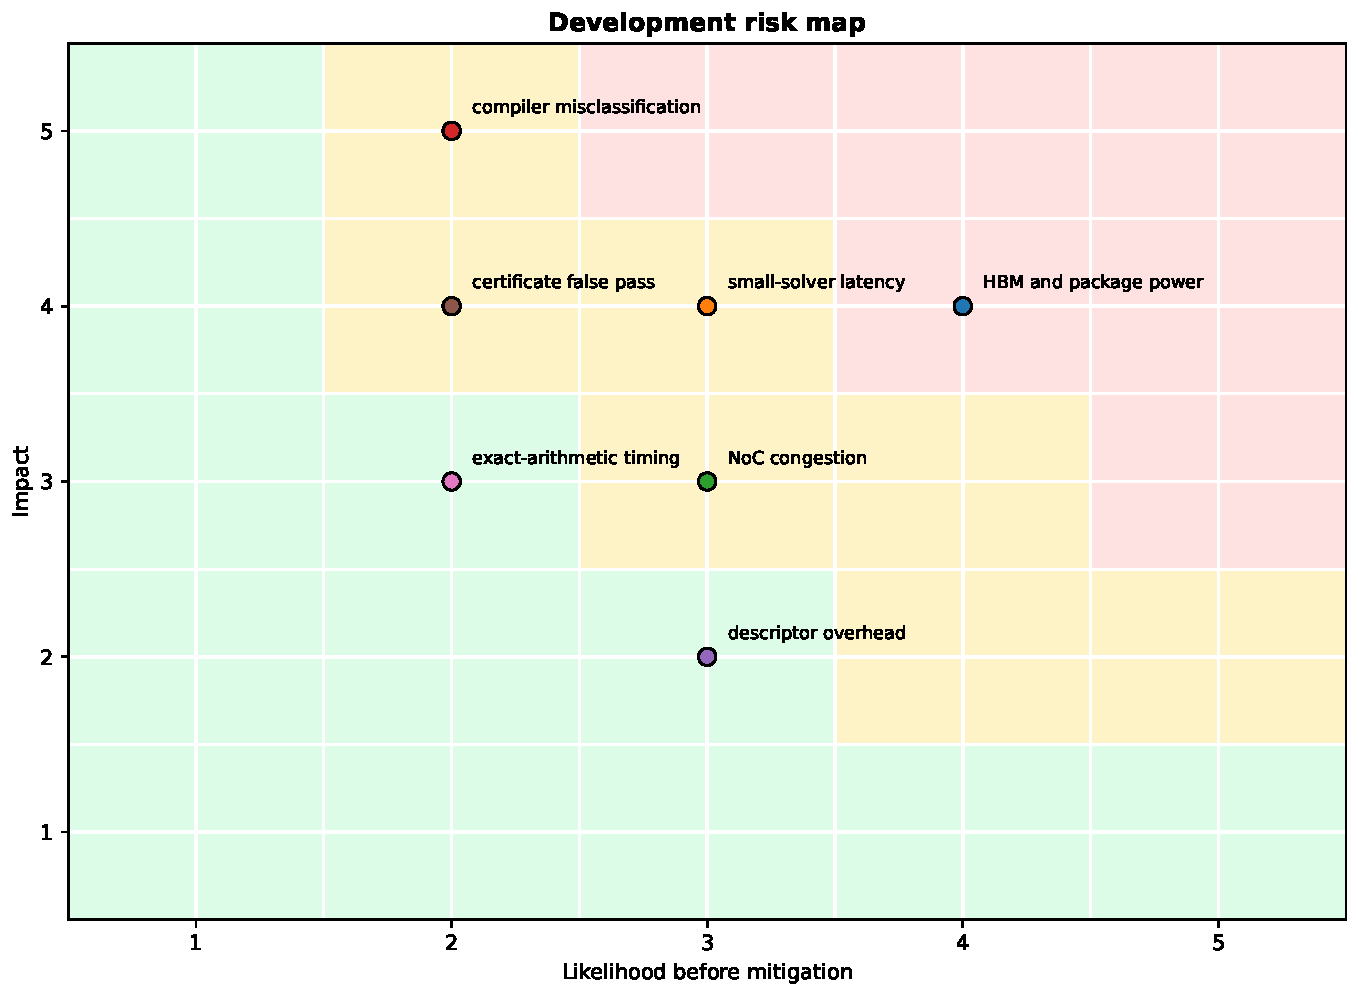
\includegraphics[width=0.86\linewidth]{35_risk_matrix.pdf}
\caption{Development risk map. Values are planning judgments rather than measured frequencies.}
\end{figure}

\section{Architecture freeze checklist}
The following items should be frozen before production RTL begins.
\begin{enumerate}
\item Packet, transfer, atlas, representation, and certificate descriptor semantics
\item Packet IR representation forms and output contracts
\item Packet-warp and Packet Streaming Multiprocessor scheduling rules
\item command and completion-record formats
\item commit and replay rules
\item supported numerical formats and rounding behavior
\item minimum transform, factor, and solver operation set
\item CUDA and PRISM backend conformance tests
\item error and exception reporting
\end{enumerate}
SRAM bank count, issue width, NoC virtual channels, exact root-solver implementation, and final DVFS domains may remain implementation choices until synthesis and floorplanning begin.

\chapter{What would count as success}

The chip should be judged against claims that can be measured:
\begin{enumerate}
\item structured operations move fewer bytes than an explicit-array route
\item BDLR, PMR--GEMM, and regular block-sparse graphs sustain useful Packet Streaming Multiprocessor occupancy
\item transform analysis and synthesis remain exact within the declared numerical format
\item mixed-precision results satisfy their packet bounds
\item local refinement changes only the local descriptor region
\item edge recovery keeps the small algebraic chain resident
\item Bayesian portfolios reuse state matrices rather than reloading them per model
\item negative controls are routed to CUDA, a general device, or a generic leaf when PRISM is not the better path
\end{enumerate}

A successful PRISM chip would not prove the calculus. The mathematics already supplies the contracts. The hardware question is whether keeping those contracts visible saves enough scheduling, movement, and handoff cost beyond the already optimized CUDA implementation to justify a dedicated machine.

\chapter{Final architecture statement}
The final design follows one principle:
\[
\boxed{
\text{Do not materialize, move, or schedule structure that the calculus has already declared inactive.}
}
\]
The machine executes
\[
\begin{aligned}
\text{seed object}
&\longrightarrow \text{Packet IR}\\
&\longrightarrow \text{mixed-representation plan}\\
&\longrightarrow \text{packet warps on CUDA or PRISM}\\
&\longrightarrow \text{local refinement and synthesis}\\
&\longrightarrow \text{certificate and commit}.
\end{aligned}
\]
PRISM-1 is a CUDA-like packet-programmable processor, not a dense-matrix preservation machine. Its hardware state may be a factor graph, transform chain, packet tree, sparse operator, explicit array, or mixture of those forms. The requested output contract determines what must be returned.

The CUDA backend proves that the calculus can run before silicon. The FPGA and ASIC question is narrower and testable: whether resident packet scheduling, factor reuse, transform-to-solver handoff, local refinement, and certificate-gated execution add enough value beyond the packet CUDA path.

\appendix
\chapter{Reference data sheet}
\begin{longtable}{L{0.42\linewidth}L{0.46\linewidth}}
\toprule
Item & PRISM-1 reference target \\
\midrule
\endfirsthead
\toprule
Item & PRISM-1 reference target \\
\midrule
\endhead
Compute chiplets & 4 \\
Packet Streaming Multiprocessors & 64 total, 16 per compute chiplet \\
Packet execution groups & 256 total, 4 per multiprocessor \\
Execution group & $16\times16$ matrix array plus programmable vector lanes \\
Clock & 1.5 GHz model target \\
Packet scratchpad & 2 MiB per multiprocessor across four banked regions \\
Shared SRAM & 16 MiB per compute chiplet \\
Total local and shared SRAM & 192 MiB \\
FP16 and BF16 model peak & 196.6 TFLOP/s \\
FP32 model peak & 98.3 TFLOP/s \\
FP64 model peak & 24.6 TFLOP/s \\
Transform engines & 32 \\
Small-solver engines & 16 \\
Exact arithmetic clusters & 4 \\
HBM4 & 4 stacks \\
HBM capacity & 144 GiB \\
HBM bandwidth & greater than 11.2 TB/s aggregate \\
Package links & UCIe 3.0 class at up to 64 GT/s \\
Host link & PCIe 7.0 x16 class, optional CXL \\
Power target & 500 W \\
Representation forms & explicit array, block, block sparse, low rank, BDLR, Kronecker, sparse factor chain, transform plan, packet graph \\
Output contracts & apply, compressed operator, factor graph, transform plan, explicit array \\
Software backends & CUDA compatibility backend and PRISM backend from shared Packet IR \\
\bottomrule
\end{longtable}


\chapter{Operation-to-engine map}
\begin{figure}[H]
\centering
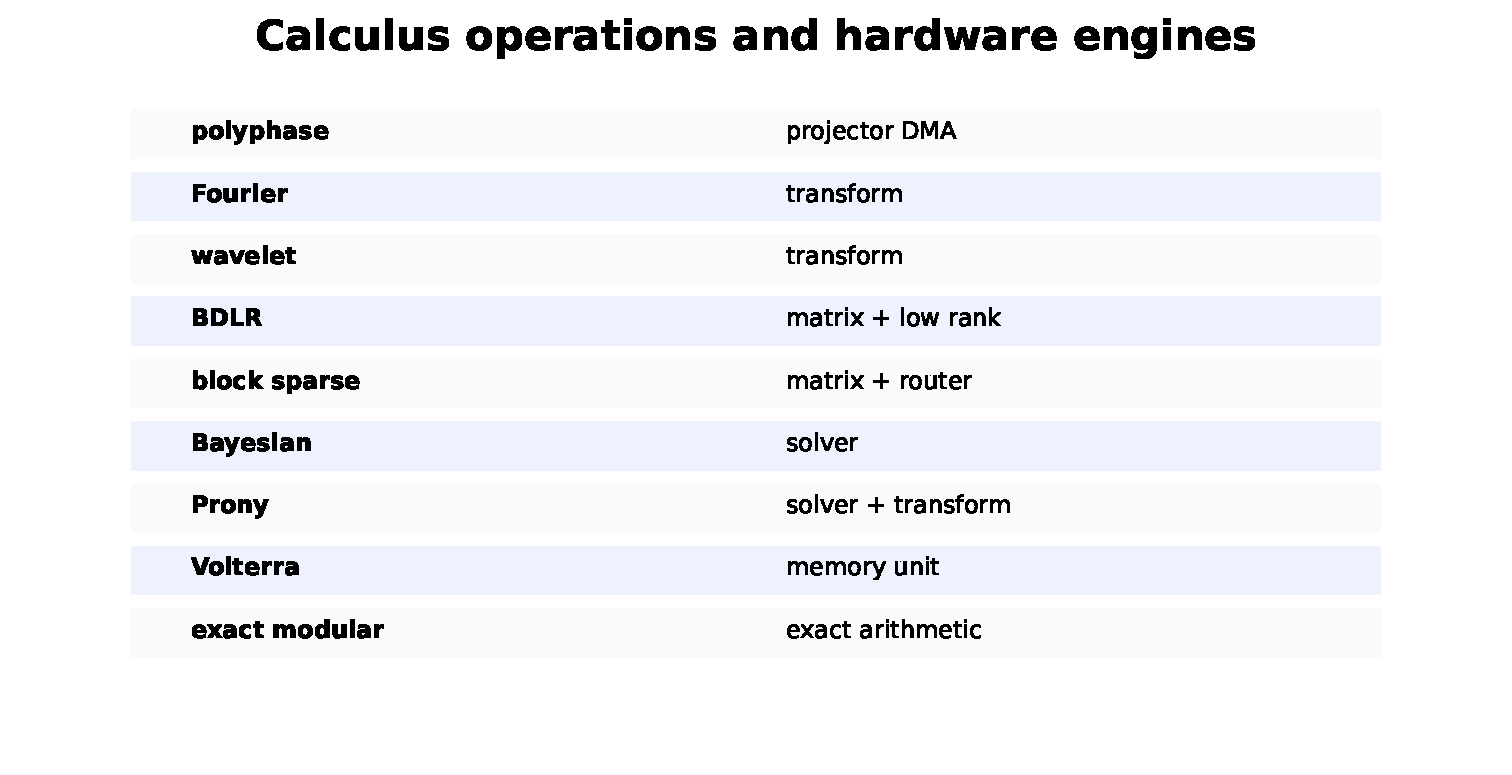
\includegraphics[width=0.96\linewidth]{13_workload_engine_map.pdf}
\caption{The main calculus operations and their primary hardware engines.}
\end{figure}

\chapter{Executable model and source layout}
The source package contains the executable architecture model, independent tests, compiler examples, documentation, generated figures, machine-readable results, and an RTL module skeleton. Raw source listings are kept in the release rather than printed across the final paper.

\begin{longtable}{L{0.32\linewidth}L{0.58\linewidth}}
\toprule
Path & Role \\
\midrule
\endfirsthead
\toprule
Path & Role \\
\midrule
\endhead
\texttt{prism\_chip\_model.py} & Behavioral operations, roofline model, sensitivity sweeps, figures, and self-tests \\
\texttt{tests/} & Independent contract tests \\
\texttt{compiler\_ir/} & BDLR, PMR--GEMM, unknown-edge, and PR-LASM graph examples \\
\texttt{rtl\_skeleton/} & Descriptor, queue, scoreboard, packet directory, representation router, PSM scheduler, execution group, residual, commit, and top-level module boundaries \\
\texttt{docs/} & Data sheet, command specification, compiler notes, and microarchitecture notes \\
\texttt{results/} & Machine-readable architecture results \\
\bottomrule
\end{longtable}

\chapter{RTL module boundaries}
\begin{longtable}{L{0.34\linewidth}L{0.56\linewidth}}
\toprule
Module & Responsibility \\
\midrule
\endfirsthead
\toprule
Module & Responsibility \\
\midrule
\endhead
\texttt{prism\_descriptor\_pkg} & Command opcodes and packed descriptor types \\
\texttt{prism\_command\_fifo} & Command-ring buffering and flow control \\
\texttt{prism\_token\_scoreboard} & Dependency-token readiness and completion tracking \\
\texttt{prism\_packet\_directory} & Packet validity, provisional state, commit state, and storage location \\
\texttt{prism\_residual\_accumulator} & Wide residual accumulation \\
\texttt{prism\_commit\_controller} & Certificate comparison, commit, replay, and abort decisions \\
\texttt{prism\_representation\_router} & Dispatch among block, factor, transform, solver, packet-graph, and generic leaves \\
\texttt{prism\_psm\_scheduler} & Packet-warp issue, dependency tracking, replay-region control, and execution-group assignment \\
\texttt{prism\_execution\_group} & Matrix, vector, selector, reduction, and provisional-result boundary for one execution group \\
\texttt{prism\_tile\_shell} & Compatibility shell for one execution group during staged RTL development \\
\texttt{prism\_top} & Queue, scoreboard, packet directory, and completion interface shell \\
\bottomrule
\end{longtable}

The module set remains a boundary specification rather than production RTL. A production implementation still requires bit-accurate datapaths, interface IP, reset and clock-domain design, verification properties, synthesis, timing closure, and physical design.

\chapter{Implementation baseline}
\section*{Internal algorithmic basis}
The architecture integrates three existing project components.
\begin{itemize}
\item Dense Transfer Algebra supplies PMR--GEMM, compatible middle bases, Kronecker rules, sparse factor chains, and the generic fallback.
\item Projector-Resolved Seed Calculus VIII supplies exact block, BDLR, compressed-product, Woodbury, packet-Krylov, mixed-precision, amortization, and CUDA Graph results.
\item The CUDA backend supplies the working software route through grouped matrix kernels, FFT and sparse libraries, asynchronous transfers, graph replay, and packetwise certification.
\end{itemize}
These algorithms are architecture inputs. PRISM does not claim them as consequences of the chip.

The package assumptions use current public baselines from the UCIe Consortium, PCI-SIG, Micron, and RISC-V International. The relevant values are the 48 and 64 GT/s classes in UCIe 3.0, the 128 GT/s PCIe 7.0 host-link class, Micron's 2048-bit HBM4 interface with bandwidth above 2.8 TB/s per stack, and the ratified RISC-V Vector 1.0 programming model. These sources establish a plausible interconnect, memory, and control baseline. They do not validate the PRISM microarchitecture.

\end{document}
